\graphicspath{{chapters/method/figures/}}

\subsection{Optimization frameworks}
\begin{frame}\frametitle{Optimization frameworks}
\begin{table}
%\label{table:ACM-ML}
\begin{scriptsize}
\begin{tabular}{ll c ccc}
    
             						&                    	& ML+MRF & \multicolumn{3}{c}{ACM} \\ \cmidrule{4-6}
             						&                    	&	       			 & Snakes 	& LevelSets 	&   ACWE \\ \toprule
    Spatially  				& continuous	&        			 & \ch 			& \ch 				&      \ch       \\ \cmidrule{2-6}
             						& discrete 		& \ch    		 &    	 			&     					&  \\ \midrule
    \multicolumn{2}{l}{Contour control or modeling} & 		& \ch 	&  \ch 	&   \ch       \\ \midrule
    \multicolumn{2}{l}{Data model} & {\color{red} \textbf{\ch}}    &     &   &  \\ \midrule
    \multicolumn{2}{l}{Need of initialization} & &\ch    &\ch    &  \\ \midrule
    \multicolumn{2}{l}{Topology changes} &\ch & &\ch &\ch   \\ 
    \bottomrule
\end{tabular}
\caption{Optimization methods characteristics}
\end{scriptsize}
\end{table}
\end{frame}

\subsection{Discrete optimization framework: general view}
\begin{frame}\frametitle{Labeling problem and system outline}
\vspace{-5pt}
\begin{footnotesize}
\begin{small}
\begin{block}{Labeling problem formulation}
\begin{equation*}
U(\omega) = \sum_{s\in S} D_s(\omega_s) + \sum_{s}\sum_{r \in \mathcal{N}_{s}} V_{s,r}(\omega_s,\omega_r)
\end{equation*} 
\end{block}
\end{small}
%\onslide<1|handout:0>
\vspace{-5pt}
\begin{columns}
\begin{column}{.48\textwidth}
\begin{itemize}
\item $\mathcal{S},\mathcal{L}, \mathcal{W}$
\item $\omega \in W \text{\, {\scriptsize where } \,} \omega_s = l \in \mathcal{L}$
\end{itemize}
\end{column}
\begin{column}{.48\textwidth}
\begin{itemize}
\item $D_s(\cdot)$
\item $\sum_{r \in \mathcal{N}_{s}} V_{s,r}(\cdot,\cdot)$,
\end{itemize}
\end{column}
\end{columns}
\end{footnotesize}
%\vspace{-10pt}
\begin{figure}[htbp]
\centering
\begin{scriptsize}
%
\begin{tikzpicture}[scale=.5]
\def\sqHalfsize{.4}
\def\pcolor{black}
%\newcounter{ii}
\setcounter{ii}{1}

% Draw the possibilities
\foreach \a in {0,1}  \foreach \b  in {0,1}  \foreach \c in {0,1} \foreach \d in {0,1} {
\ifthenelse{ 1 = \a }{\draw[pattern=north east lines, pattern color=\pcolor] (\value{ii},0) rectangle +(-\sqHalfsize,\sqHalfsize);}{ \draw[] (\value{ii},0) rectangle +(-\sqHalfsize,\sqHalfsize);}
\ifthenelse{ 1 = \b }{\draw[pattern=north east lines, pattern color=\pcolor] (\value{ii},0) rectangle +(\sqHalfsize,\sqHalfsize);}{ \draw[] (\value{ii},0) rectangle +(\sqHalfsize,\sqHalfsize);}
\ifthenelse{ 1 = \c }{\draw[pattern=north east lines, pattern color=\pcolor] (\value{ii},0) rectangle +(-\sqHalfsize,-\sqHalfsize);}{ \draw[] (\value{ii},0) rectangle +(-\sqHalfsize,-\sqHalfsize);}
\ifthenelse{ 1 = \d }{\draw[pattern=north east lines, pattern color=\pcolor] (\value{ii},0) rectangle +(\sqHalfsize,-\sqHalfsize);}{ \draw[] (\value{ii},0) rectangle +(\sqHalfsize,-\sqHalfsize);}

%\node[] at (\value{i},-1) {$\arabic{i}$};
\stepcounter{ii} 
}

% Draw the axes
\draw (0.2,.8) -- (17,.8) node [anchor=north west] {$W$};
\draw[->]	   (0.2,.8) -- (.2, 5) node [anchor=north east] {$U(\omega)$};

% Draw the costs
\def\costs{2/2, 1/3 , 2/3 , 1/2 ,2/3 ,1/1 ,2/3 ,1/3 ,2/3 ,2/3 ,3/1 ,2/3 ,3/2 ,2/3 ,3/3 ,2/2 }
\foreach \dataX/\smoothX [count=\idx] in \costs
{
	\def\smooth{.5*\smoothX}
	\def\data{.5*\dataX}
	\draw[color=blue] (\idx,.8) -- (\idx,{.8+\smooth})  ({\idx - 0.2},{.8+\smooth}) -- ({\idx + 0.2},{.8+\smooth});
	\draw[color=red,-o] (\idx,{.8+\smooth}) -- (\idx,{.8+\smooth+\data});
}
{\scalefont{.8}
\draw (12,0) node (ref) {};
\draw [color=red] (17,5) node[anchor=north east,color=black] (dlabel) {\emph{data term cost}} (dlabel.west) -- (dlabel.west -| ref);
\draw [color=blue](dlabel.south east) ++(0,.2) node[anchor=north east,color=black] (slabel) {\emph{smoothing term cost}} (slabel.west) -- (slabel.west -| ref);
}
\end{tikzpicture} 

\includegraphics[height=.4\textheight]{toy.pdf}
\end{scriptsize}
\caption{ Toy example illustrating the data and pairwise costs of the solution space $\mathcal{W}$ .}
\label{fig:toyFigure}
\end{figure}

%\onslide<2|handout:0>
%\vspace{-20pt}
%\begin{figure}[htbp]
%\centering
%\begin{scriptsize}
%\begin{tikzpicture}[y=0.80pt, x=0.8pt,yscale=-1, inner sep=0pt, outer sep=0pt,scale=.7]
\begin{scope}[shift={(0,426.0)},xscale=0.100,yscale=-0.100,fill=black]% g3151
  % path3155
  \path[fill] (3313.7800,2904.6857) .. controls (3298.4191,2907.5563) and
    (3283.6417,2913.1980) .. (3268.0572,2915.0394) .. controls
    (3231.8571,2921.2493) and (3193.8308,2921.8192) .. (3160.0275,2937.3643) ..
    controls (3150.8918,2941.8618) and (3142.5452,2950.6960) ..
    (3143.4870,2961.5522) .. controls (3143.8632,2978.0269) and
    (3152.4900,2992.6930) .. (3159.5483,3007.1873) .. controls
    (3166.5657,3020.5272) and (3175.0648,3033.3992) .. (3179.1556,3047.9733) ..
    controls (3179.1656,3054.5883) and (3171.3230,3058.2032) ..
    (3165.6049,3056.1957) .. controls (3151.6888,3053.9186) and
    (3138.9017,3047.3425) .. (3125.6733,3042.7453) .. controls
    (3083.0760,3025.9731) and (3041.8008,3004.8937) .. (2997.5927,2992.8700) ..
    controls (2990.6249,2991.3703) and (2983.4045,2992.8480) ..
    (2977.4680,2996.6266) .. controls (2966.0414,3001.8146) and
    (2952.7537,3002.2959) .. (2942.1444,3009.1998) .. controls
    (2930.2402,3018.7786) and (2927.1326,3035.1104) .. (2926.6542,3049.7170) ..
    controls (2925.4506,3083.6992) and (2936.4643,3116.6304) ..
    (2950.3660,3147.1360) .. controls (2969.2999,3186.5051) and
    (2997.0345,3221.9629) .. (3033.0313,3246.8050) .. controls
    (3054.6228,3259.9720) and (3079.5877,3266.4157) .. (3104.2582,3271.0654) ..
    controls (3124.6023,3274.1945) and (3145.6523,3271.3888) ..
    (3164.6256,3263.5079) .. controls (3187.5814,3254.8022) and
    (3209.7881,3242.2516) .. (3226.4301,3224.0251) .. controls
    (3228.9615,3220.7734) and (3232.3090,3216.7168) .. (3231.5756,3212.4397) ..
    controls (3227.9438,3209.1403) and (3222.4632,3211.0589) ..
    (3218.0440,3209.6989) .. controls (3205.8344,3207.3165) and
    (3198.0717,3196.5428) .. (3190.9775,3187.2939) .. controls
    (3187.9299,3183.9140) and (3183.9049,3179.6779) .. (3179.1556,3179.8761) ..
    controls (3181.4843,3189.5988) and (3190.4183,3196.0721) ..
    (3196.0307,3203.9951) .. controls (3199.9739,3209.2047) and
    (3203.7017,3216.1091) .. (3200.6410,3222.6554) .. controls
    (3197.9112,3228.9646) and (3191.3971,3234.3017) .. (3184.3688,3234.1552) ..
    controls (3177.7196,3233.3722) and (3174.8906,3226.4540) ..
    (3171.2782,3221.8505) .. controls (3168.9266,3219.9847) and
    (3164.0026,3219.0747) .. (3162.5958,3222.3871) .. controls
    (3163.2919,3226.0591) and (3164.8400,3229.6987) .. (3163.5541,3233.4844) ..
    controls (3162.3133,3240.2243) and (3155.4840,3247.1502) ..
    (3148.2211,3244.6201) .. controls (3146.8784,3243.9608) and
    (3145.8568,3242.8568) .. (3144.9628,3241.6876) .. controls
    (3142.7564,3246.1814) and (3137.4304,3247.0420) .. (3132.9091,3246.8731) ..
    controls (3122.8547,3247.7688) and (3110.5304,3246.6228) ..
    (3104.6943,3237.3369) .. controls (3099.1113,3227.2726) and
    (3103.3497,3215.2780) .. (3107.2857,3205.4329) .. controls
    (3111.6786,3194.6353) and (3118.9261,3184.3101) .. (3122.0207,3173.4362) ..
    controls (3116.4336,3175.2049) and (3113.9327,3181.0890) ..
    (3110.4442,3185.3769) .. controls (3101.7564,3198.6460) and
    (3097.7726,3215.1537) .. (3086.3904,3226.5270) .. controls
    (3078.1105,3232.5454) and (3065.9710,3227.4308) .. (3061.4358,3219.0330) ..
    controls (3057.7179,3213.0542) and (3058.4066,3204.7578) ..
    (3060.9566,3199.0233) .. controls (3054.7764,3202.9981) and
    (3050.3084,3209.6018) .. (3042.9403,3211.5581) .. controls
    (3038.3333,3213.3543) and (3032.0542,3211.1878) .. (3031.2680,3205.8849) ..
    controls (3029.9208,3198.4603) and (3035.4840,3192.1816) ..
    (3039.0303,3186.2585) .. controls (3044.6415,3178.5317) and
    (3051.8064,3172.0530) .. (3057.9475,3164.8114) .. controls
    (3045.5652,3171.4696) and (3036.0724,3182.3678) .. (3023.1990,3188.2326) ..
    controls (3017.4285,3191.1458) and (3010.7453,3194.7546) ..
    (3004.1284,3192.8134) .. controls (2997.9825,3190.3399) and
    (2996.7314,3182.2709) .. (2999.6052,3176.8479) .. controls
    (3004.1092,3167.0517) and (3013.1197,3160.2466) .. (3021.4939,3153.8367) ..
    controls (3033.2161,3145.2808) and (3047.0549,3139.6380) ..
    (3058.0817,3130.2161) .. controls (3059.7710,3128.5596) and
    (3061.4771,3126.7570) .. (3062.3941,3124.5237) .. controls
    (3055.6214,3125.4595) and (3050.2470,3130.3803) .. (3044.3849,3133.5655) ..
    controls (3030.7974,3142.4125) and (3018.3494,3154.9234) ..
    (3001.7901,3157.7390) .. controls (2993.4372,3156.8971) and
    (2988.8600,3147.6139) .. (2989.0637,3139.8951) .. controls
    (2988.4418,3129.1755) and (2995.4511,3118.8891) .. (3004.8567,3114.5764) ..
    controls (3004.1555,3112.8615) and (3001.2729,3114.2636) ..
    (2999.8735,3114.2314) .. controls (2994.7267,3115.7044) and
    (2988.3980,3117.6025) .. (2983.8504,3113.6372) .. controls
    (2977.8662,3108.9754) and (2979.6440,3099.5380) .. (2984.4254,3094.6434) ..
    controls (2989.4057,3088.4344) and (2997.9009,3086.3950) ..
    (3004.0134,3082.0894) .. controls (2990.3142,3079.1555) and
    (2975.7441,3082.5522) .. (2962.2691,3078.4861) .. controls
    (2957.6738,3075.3371) and (2961.6264,3067.8200) .. (2966.6582,3068.0021) ..
    controls (2985.1479,3063.2239) and (3004.5083,3056.9151) ..
    (3023.6781,3061.1406) .. controls (3026.7291,3061.1406) and
    (3027.1133,3057.6766) .. (3027.0897,3055.3523) .. controls
    (3027.6718,3049.7381) and (3030.8141,3042.6725) .. (3037.3437,3042.5875) ..
    controls (3048.4548,3042.2118) and (3057.6616,3049.5462) ..
    (3067.6473,3053.2529) .. controls (3083.2979,3060.4942) and
    (3099.9974,3067.2178) .. (3111.9200,3080.1536) .. controls
    (3115.0365,3084.5403) and (3114.6738,3090.3824) .. (3113.3575,3095.2375) ..
    controls (3115.4257,3099.6625) and (3121.4569,3098.7899) ..
    (3125.0958,3097.0226) .. controls (3142.1593,3090.9247) and
    (3160.5712,3091.4888) .. (3178.4847,3090.9826) .. controls
    (3185.3033,3090.8896) and (3192.1235,3090.7799) .. (3198.9352,3090.4460) ..
    controls (3210.8727,3116.8231) and (3223.9199,3142.7961) ..
    (3233.9138,3169.9480) .. controls (3233.7184,3176.1775) and
    (3225.3564,3178.4566) .. (3220.6891,3175.4104) .. controls
    (3215.7129,3173.6328) and (3211.6954,3169.7193) .. (3206.4293,3168.7021) ..
    controls (3213.0716,3175.5033) and (3222.3411,3179.1384) ..
    (3231.7230,3179.9797) .. controls (3238.9414,3179.5336) and
    (3245.8001,3184.8874) .. (3247.0620,3191.9892) .. controls
    (3249.3500,3201.9146) and (3254.0481,3211.2855) .. (3257.9461,3220.6683) ..
    controls (3269.3024,3245.0280) and (3281.4552,3269.1347) ..
    (3294.0473,3292.8623) .. controls (3304.6981,3312.3191) and
    (3316.0320,3331.5420) .. (3330.1864,3348.6933) .. controls
    (3335.0862,3351.9760) and (3340.9951,3354.2455) .. (3346.8803,3354.8074) ..
    controls (3358.4813,3354.2560) and (3368.6438,3347.3655) ..
    (3378.9616,3342.4805) .. controls (3408.5597,3326.9861) and
    (3438.7306,3311.8167) .. (3471.4359,3304.1687) .. controls
    (3487.4044,3299.8977) and (3504.5518,3295.0887) .. (3516.4067,3282.9336) ..
    controls (3521.7491,3276.1245) and (3520.5933,3266.3715) ..
    (3516.1575,3259.4165) .. controls (3507.6188,3243.1376) and
    (3493.9909,3230.3101) .. (3485.0449,3214.3195) .. controls
    (3462.7497,3179.2071) and (3441.6750,3143.2697) .. (3422.1551,3106.5590) ..
    controls (3393.6961,3052.6348) and (3369.0948,2996.7942) ..
    (3342.1715,2942.1082) .. controls (3335.8487,2930.1099) and
    (3329.8937,2917.5637) .. (3320.6224,2907.5031) .. controls
    (3318.7393,2905.8773) and (3316.3472,2904.5204) .. (3313.7800,2904.6857) --
    cycle(3305.2318,2935.2176) .. controls (3312.4162,2934.7409) and
    (3317.5498,2944.7037) .. (3312.4576,2950.0716) .. controls
    (3304.9863,2962.6653) and (3289.7961,2966.8037) .. (3277.7473,2973.6653) ..
    controls (3274.8826,2975.1888) and (3279.7400,2974.8015) ..
    (3280.9672,2974.9878) .. controls (3292.0677,2975.0798) and
    (3303.7451,2969.2938) .. (3314.5275,2973.6845) .. controls
    (3320.0682,2977.0317) and (3318.0622,2986.0987) .. (3312.4767,2988.2701) ..
    controls (3301.9668,2996.3673) and (3287.1937,2997.0823) ..
    (3277.0189,3005.1940) .. controls (3284.7591,3008.5622) and
    (3294.1393,3007.5437) .. (3301.2305,3012.7226) .. controls
    (3302.1864,3012.9795) and (3304.8100,3015.9256) .. (3303.5452,3013.4930) ..
    controls (3301.4914,3008.0472) and (3300.5737,3000.7209) ..
    (3305.7110,2996.6842) .. controls (3310.6074,2992.7059) and
    (3317.4605,2995.6867) .. (3322.3090,2998.2366) .. controls
    (3332.0688,3004.1782) and (3338.2662,3014.8189) .. (3341.0346,3025.6445) ..
    controls (3342.3249,3031.0841) and (3339.1178,3037.3727) ..
    (3333.3297,3038.2176) .. controls (3325.5220,3039.9112) and
    (3318.4641,3034.6269) .. (3313.5500,3029.1711) .. controls
    (3314.8043,3033.9548) and (3313.2583,3039.2736) .. (3309.0268,3042.0317) ..
    controls (3295.9104,3052.0689) and (3277.7972,3054.1341) ..
    (3266.0558,3066.1046) .. controls (3265.4855,3066.7121) and
    (3264.1707,3069.0247) .. (3266.0368,3067.6571) .. controls
    (3277.3001,3063.3268) and (3287.3433,3055.9312) .. (3299.2014,3053.0692) ..
    controls (3308.7945,3049.7559) and (3320.7708,3049.7643) ..
    (3328.4999,3057.1732) .. controls (3329.6160,3058.2458) and
    (3330.8266,3059.7415) .. (3329.7649,3057.2881) .. controls
    (3328.3509,3051.7982) and (3326.9664,3044.0862) .. (3332.5632,3040.4217) ..
    controls (3337.4688,3037.2058) and (3343.5180,3040.8657) ..
    (3347.5282,3043.9335) .. controls (3353.4571,3049.1560) and
    (3358.0921,3055.9153) .. (3361.6385,3062.9613) .. controls
    (3364.3271,3068.8905) and (3363.2527,3077.4137) .. (3356.6745,3080.2111) ..
    controls (3349.9478,3083.3758) and (3341.7942,3079.4680) ..
    (3338.4281,3073.2537) .. controls (3337.7294,3072.6365) and
    (3336.1206,3069.6862) .. (3336.1090,3070.4554) .. controls
    (3337.4096,3076.7228) and (3334.8742,3083.6403) .. (3329.2091,3086.8809) ..
    controls (3326.5222,3088.5598) and (3328.8378,3091.8364) ..
    (3331.2599,3091.9601) .. controls (3334.6362,3092.4150) and
    (3337.4355,3089.4240) .. (3340.9581,3090.1776) .. controls
    (3346.2885,3090.0672) and (3351.3578,3094.7001) .. (3350.4071,3100.2207) ..
    controls (3350.0497,3107.7187) and (3342.9281,3113.2378) ..
    (3338.5240,3117.4896) .. controls (3348.0003,3119.4249) and
    (3359.6803,3120.4569) .. (3365.2418,3129.5644) .. controls
    (3368.5909,3136.8515) and (3363.1147,3144.7681) .. (3356.9045,3148.3666) ..
    controls (3344.5912,3157.2817) and (3329.1389,3160.5922) ..
    (3316.7701,3169.5071) .. controls (3334.8913,3167.9049) and
    (3351.0441,3156.5237) .. (3369.5159,3157.0873) .. controls
    (3378.6730,3158.3356) and (3384.5236,3167.8823) .. (3384.7148,3176.5987) ..
    controls (3384.9966,3184.8075) and (3377.3974,3191.0465) ..
    (3369.6309,3191.5676) .. controls (3367.2117,3191.9128) and
    (3363.5432,3191.2743) .. (3363.1144,3194.5576) .. controls
    (3362.2617,3197.2134) and (3365.6759,3195.0910) .. (3366.9285,3194.9217) ..
    controls (3374.6136,3192.0857) and (3383.5876,3187.4435) ..
    (3391.6339,3191.7784) .. controls (3399.4221,3196.2531) and
    (3400.5047,3208.9616) .. (3392.9372,3214.1839) .. controls
    (3389.0427,3218.0670) and (3382.8676,3218.7838) .. (3378.5625,3221.2946) ..
    controls (3388.3382,3221.4384) and (3398.8818,3216.5518) ..
    (3408.1170,3221.7738) .. controls (3414.2077,3225.3162) and
    (3415.2150,3233.8321) .. (3411.9119,3239.6176) .. controls
    (3407.6403,3249.2115) and (3398.6409,3255.3115) .. (3391.4998,3262.6556) ..
    controls (3399.4202,3258.8670) and (3408.3767,3253.0084) ..
    (3417.4510,3256.6948) .. controls (3429.0151,3261.1556) and
    (3435.4621,3272.5343) .. (3444.8589,3279.9628) .. controls
    (3447.3346,3281.8755) and (3446.8762,3285.9806) .. (3443.7467,3286.8717) ..
    controls (3417.6075,3298.8195) and (3393.1339,3315.2624) ..
    (3365.1077,3322.6079) .. controls (3356.9932,3323.9377) and
    (3348.1286,3320.0777) .. (3344.5997,3312.4690) .. controls
    (3333.5856,3295.0384) and (3325.1175,3276.1191) .. (3315.5729,3257.8303) ..
    controls (3282.9909,3192.2209) and (3252.6431,3125.5542) ..
    (3223.9843,3058.1752) .. controls (3212.6619,3030.7251) and
    (3200.8110,3003.3647) .. (3185.6914,2977.9203) .. controls
    (3182.5805,2971.6995) and (3179.4176,2964.0279) .. (3182.4140,2957.2015) ..
    controls (3186.5202,2950.7629) and (3195.1567,2950.9482) ..
    (3201.7337,2948.9599) .. controls (3231.3779,2942.8415) and
    (3261.9078,2943.1769) .. (3291.6239,2937.5176) .. controls
    (3296.1581,2936.7435) and (3300.6906,2935.9362) .. (3305.2320,2935.2176) --
    cycle(2978.1580,3020.0862) .. controls (2992.3013,3020.6935) and
    (3007.7770,3023.4946) .. (3018.1391,3033.8285) .. controls
    (3021.8056,3038.9690) and (3018.1991,3046.9459) .. (3011.9869,3047.7466) ..
    controls (2999.9235,3052.0893) and (2986.4546,3051.4796) ..
    (2974.1714,3048.4141) .. controls (2967.0789,3045.8168) and
    (2962.1242,3037.2800) .. (2965.4124,3029.9952) .. controls
    (2967.3484,3024.6535) and (2972.2993,3020.2467) .. (2978.1580,3020.0862) --
    cycle(3362.2709,3081.3802) .. controls (3373.3018,3080.4734) and
    (3380.1459,3096.2833) .. (3372.0457,3103.7282) .. controls
    (3367.7607,3107.5304) and (3360.9081,3105.7351) .. (3357.8243,3101.2749) ..
    controls (3352.9454,3096.7662) and (3350.9267,3087.3313) ..
    (3357.1151,3083.0285) .. controls (3358.6418,3082.0150) and
    (3360.4418,3081.4667) .. (3362.2709,3081.3802) -- cycle(3373.8857,3106.4882)
    .. controls (3388.8373,3106.5722) and (3399.3052,3126.1936) ..
    (3390.5987,3138.4768) .. controls (3386.4711,3144.1422) and
    (3377.2103,3143.7513) .. (3373.2148,3138.1510) .. controls
    (3367.6130,3132.2526) and (3364.3577,3123.8415) .. (3364.5134,3115.7838) ..
    controls (3365.2640,3111.1341) and (3368.9306,3106.7322) ..
    (3373.8857,3106.4882) -- cycle(3396.5403,3144.7825) .. controls
    (3406.3606,3146.2860) and (3410.9905,3156.4602) .. (3414.5184,3164.6005) ..
    controls (3416.9206,3170.1011) and (3414.6810,3178.6051) ..
    (3407.9251,3179.3203) .. controls (3399.7822,3180.5621) and
    (3393.5448,3173.3139) .. (3390.5796,3166.6130) .. controls
    (3387.2273,3160.1265) and (3386.4085,3150.3290) .. (3393.0712,3145.7025) ..
    controls (3394.1369,3145.1286) and (3395.3229,3144.7838) ..
    (3396.5403,3144.7825) -- cycle(3415.1317,3179.4736) .. controls
    (3423.0938,3179.0934) and (3432.1234,3185.8464) .. (3430.4456,3194.4617) ..
    controls (3430.1198,3196.7435) and (3428.9805,3198.8666) ..
    (3427.3023,3200.4416) .. controls (3438.2701,3201.8923) and
    (3445.3972,3212.8032) .. (3447.0436,3223.0196) .. controls
    (3447.8426,3233.1604) and (3437.2103,3243.4854) .. (3427.0723,3239.9051) ..
    controls (3419.6546,3235.9579) and (3417.2931,3226.8570) ..
    (3415.9941,3219.1672) .. controls (3415.3611,3214.0224) and
    (3415.6283,3208.3173) .. (3418.9266,3204.0832) .. controls
    (3411.8719,3204.4073) and (3404.8744,3199.2039) .. (3402.9227,3192.4301) ..
    controls (3401.0893,3186.7524) and (3405.4654,3180.7944) ..
    (3411.1259,3179.9336) .. controls (3412.4383,3179.5953) and
    (3413.7808,3179.5288) .. (3415.1317,3179.4736) -- cycle(3146.2661,3198.7358)
    .. controls (3139.1092,3200.6029) and (3136.5625,3209.2087) ..
    (3136.9320,3215.8514) .. controls (3137.0250,3221.4717) and
    (3139.6802,3227.0291) .. (3142.9120,3231.2994) .. controls
    (3143.1397,3220.3692) and (3147.5198,3209.6532) .. (3146.2661,3198.7358) --
    cycle(3450.8961,3238.4869) .. controls (3462.8164,3239.7991) and
    (3470.6932,3250.2689) .. (3476.8473,3259.5314) .. controls
    (3480.7673,3266.3901) and (3481.0939,3277.0428) .. (3473.6082,3281.5536) ..
    controls (3465.5205,3286.2544) and (3455.5797,3282.0319) ..
    (3449.0369,3276.5896) .. controls (3441.9424,3271.1752) and
    (3434.7418,3263.6509) .. (3434.4897,3254.2033) .. controls
    (3435.3590,3245.9818) and (3442.7416,3239.1664) .. (3450.8961,3238.4869) --
    cycle;

  % path3157
  \path[fill] (4239.9173,2773.4920) .. controls (4233.9096,2773.6027) and
    (4228.5025,2776.9426) .. (4225.0059,2781.6568) .. controls
    (4216.6190,2787.5104) and (4204.1764,2783.8576) .. (4196.9272,2791.9300) ..
    controls (4188.1907,2800.0713) and (4178.0209,2806.3569) ..
    (4167.3452,2811.5409) .. controls (4118.7531,2837.1079) and
    (4066.0618,2854.3661) .. (4018.4874,2882.0576) .. controls
    (3999.9728,2892.3860) and (3981.1069,2902.3466) .. (3960.8552,2908.8256) ..
    controls (3949.2949,2914.9850) and (3944.9213,2928.6736) ..
    (3943.2605,2940.8717) .. controls (3939.9039,2965.8020) and
    (3940.5637,2991.1548) .. (3936.2446,3015.9605) .. controls
    (3926.4084,3091.8225) and (3909.7757,3166.7199) .. (3901.9761,3242.8376) ..
    controls (3967.2810,3287.3307) and (4031.8960,3332.6877) ..
    (4096.6600,3377.9184) .. controls (4117.7444,3391.8889) and
    (4139.1609,3406.6895) .. (4163.9418,3412.9965) .. controls
    (4171.4352,3414.4088) and (4180.5676,3414.5747) .. (4186.4240,3409.0482) ..
    controls (4190.4471,3399.6255) and (4189.8687,3389.1282) ..
    (4191.4726,3379.1767) .. controls (4196.7216,3326.5402) and
    (4193.7187,3273.0432) .. (4204.2296,3221.0071) .. controls
    (4205.8762,3214.9807) and (4208.2487,3209.0695) .. (4209.7878,3202.9716) ..
    controls (4199.6536,3203.4004) and (4193.1229,3194.2286) ..
    (4186.0831,3188.3147) .. controls (4167.9740,3170.6937) and
    (4153.2290,3149.7323) .. (4136.8982,3130.4078) .. controls
    (4135.7533,3125.9748) and (4141.3796,3123.5582) .. (4142.9918,3120.0427) ..
    controls (4163.4271,3093.1484) and (4183.6147,3064.7621) ..
    (4212.9694,3047.1491) .. controls (4221.1584,3040.6411) and
    (4220.8194,3029.1383) .. (4221.8242,3019.7029) .. controls
    (4224.3016,2989.1502) and (4223.6850,2958.4540) .. (4225.4571,2927.8612) ..
    controls (4226.5198,2909.3550) and (4227.6543,2890.6374) ..
    (4232.1549,2872.6587) .. controls (4240.1869,2858.1199) and
    (4238.4303,2840.9376) .. (4240.3581,2824.9728) .. controls
    (4241.2805,2810.5664) and (4244.6050,2796.4740) .. (4245.9283,2782.1176) ..
    controls (4245.8293,2779.4123) and (4246.4289,2775.6428) ..
    (4244.7608,2773.7468) .. controls (4243.1936,2773.3042) and
    (4241.5300,2773.5453) .. (4239.9173,2773.4920) -- cycle(4215.0585,2811.4988)
    .. controls (4220.1408,2811.7144) and (4222.1176,2818.6560) ..
    (4219.5051,2822.4620) .. controls (4214.9421,2836.0923) and
    (4207.0637,2848.8469) .. (4206.3352,2863.5008) .. controls
    (4198.8825,2911.5322) and (4199.0611,2960.4306) .. (4195.3644,3008.8732) ..
    controls (4194.9727,3016.4437) and (4194.7662,3024.0369) ..
    (4193.8414,3031.5669) .. controls (4171.1224,3056.2937) and
    (4152.0480,3085.2274) .. (4123.0025,3103.1340) .. controls
    (4115.3433,3105.9335) and (4105.9775,3101.1726) .. (4099.1404,3106.7948) ..
    controls (4095.9526,3113.5030) and (4101.4194,3119.9412) ..
    (4104.2635,3125.6402) .. controls (4122.7901,3157.2198) and
    (4151.7635,3181.1849) .. (4170.1709,3212.7273) .. controls
    (4174.3396,3222.2137) and (4171.5675,3232.8659) .. (4172.2091,3242.8758) ..
    controls (4171.7034,3286.8878) and (4171.9458,3331.1093) ..
    (4168.0770,3374.9218) .. controls (4167.2526,3379.0269) and
    (4167.6591,3384.3112) .. (4164.2294,3387.2944) .. controls
    (4158.3428,3390.4576) and (4152.3656,3385.2121) .. (4147.0372,3383.0778) ..
    controls (4126.5176,3372.5052) and (4107.7679,3358.8534) ..
    (4088.2944,3346.4129) .. controls (4041.7602,3315.1398) and
    (3996.0937,3282.5195) .. (3953.2462,3246.2683) .. controls
    (3943.6520,3237.8557) and (3933.1585,3227.5576) .. (3932.6618,3213.9182) ..
    controls (3931.7169,3200.4813) and (3934.6811,3187.2585) ..
    (3935.8815,3173.9729) .. controls (3941.0994,3132.0499) and
    (3947.3676,3090.2461) .. (3955.8302,3048.8460) .. controls
    (3963.2681,3010.0756) and (3969.0707,2970.9756) .. (3973.7925,2931.8444) ..
    controls (3974.7861,2927.4259) and (3974.2400,2921.5265) ..
    (3979.1399,2919.4821) .. controls (3988.6537,2915.6914) and
    (3997.5176,2910.5117) .. (4006.8295,2906.1522) .. controls
    (4072.4917,2873.7390) and (4137.5736,2839.8511) .. (4205.9354,2813.4154) ..
    controls (4208.8867,2812.5102) and (4211.9572,2811.7584) ..
    (4215.0585,2811.4988) -- cycle;

  % path3389
  \path[fill] (2139.4449,2630.9837) .. controls (2148.5035,2631.6694) and
    (2153.1255,2640.8845) .. (2157.7872,2647.3710) .. controls
    (2180.6852,2676.3718) and (2206.1104,2703.7183) .. (2224.5052,2735.9962) ..
    controls (2224.7201,2745.3726) and (2214.9429,2751.7202) ..
    (2206.2972,2751.4443) .. controls (2168.5159,2758.7980) and
    (2129.9348,2760.5521) .. (2091.5865,2762.7716) .. controls
    (2084.8331,2762.5451) and (2076.8766,2757.6280) .. (2077.7485,2750.0451) ..
    controls (2078.4610,2741.0044) and (2085.1173,2734.0455) ..
    (2087.8411,2725.6272) .. controls (2102.5342,2694.0261) and
    (2117.5692,2662.5546) .. (2135.1709,2632.4788) .. controls
    (2136.4831,2631.7129) and (2137.8902,2631.0538) .. (2139.4449,2630.9837) --
    cycle(2233.9926,2495.2285) .. controls (2242.3073,2494.9415) and
    (2247.3679,2504.1161) .. (2246.6998,2511.6157) .. controls
    (2247.4664,2544.5491) and (2249.0311,2577.5238) .. (2248.6572,2610.4949) ..
    controls (2248.3894,2637.8410) and (2247.3419,2665.2843) ..
    (2243.9782,2692.4119) .. controls (2240.3196,2699.5974) and
    (2228.9011,2699.1977) .. (2224.8535,2692.5571) .. controls
    (2209.8292,2677.4295) and (2196.9184,2660.2047) .. (2183.8118,2643.3725) ..
    controls (2163.3785,2616.1463) and (2143.8617,2588.1213) ..
    (2124.2077,2560.3749) .. controls (2122.2005,2549.6523) and
    (2130.7721,2540.4419) .. (2139.7776,2536.1075) .. controls
    (2168.1240,2516.8437) and (2200.4946,2504.0219) .. (2233.5134,2495.2668) --
    (2233.9351,2495.2288) -- (2233.9931,2495.2288) -- cycle(2032.3242,2488.6736)
    .. controls (2041.0154,2488.8619) and (2047.5570,2496.5298) ..
    (2049.9189,2504.3517) .. controls (2071.8373,2533.0348) and
    (2098.3904,2559.0291) .. (2113.3832,2592.1904) .. controls
    (2119.4995,2609.4457) and (2113.7273,2627.9353) .. (2108.5097,2644.6759) ..
    controls (2099.1804,2672.4570) and (2087.3904,2699.4908) ..
    (2073.5982,2725.3200) .. controls (2066.7575,2737.3649) and
    (2059.4718,2749.4929) .. (2050.0141,2759.5923) .. controls
    (2037.1066,2767.4794) and (2021.2100,2763.6979) .. (2006.9884,2765.8913) ..
    controls (1975.9905,2767.5869) and (1944.5231,2770.5097) ..
    (1913.7228,2765.8003) .. controls (1906.6893,2761.0080) and
    (1906.8855,2750.9099) .. (1909.9279,2743.8548) .. controls
    (1908.9612,2733.6760) and (1899.2487,2727.6099) .. (1894.8067,2719.0057) ..
    controls (1879.0207,2695.6672) and (1863.7384,2671.4603) ..
    (1854.2496,2644.7648) .. controls (1853.0552,2634.5883) and
    (1861.9559,2626.3396) .. (1871.0968,2623.7393) .. controls
    (1906.0603,2608.8569) and (1944.9795,2609.7774) .. (1981.4772,2601.1103) ..
    controls (1991.5632,2598.5658) and (2001.8227,2595.3919) ..
    (2010.4171,2589.6999) .. controls (2007.9183,2579.0483) and
    (1998.7796,2571.4087) .. (1991.2848,2563.8916) .. controls
    (1981.7514,2554.7823) and (1972.7458,2542.7308) .. (1974.1160,2528.7700) ..
    controls (1975.8024,2514.7692) and (1987.2104,2504.3209) ..
    (1999.2622,2498.3147) .. controls (2009.5432,2493.0298) and
    (2020.6645,2489.0579) .. (2032.3242,2488.6740) -- cycle(1813.8853,2440.6427)
    .. controls (1842.6528,2440.5637) and (1860.8854,2427.5974) ..
    (1889.6325,2428.4407) .. controls (1910.5149,2471.1580) and
    (1946.9746,2526.2040) .. (1961.5045,2571.8172) .. controls
    (1960.1723,2582.8467) and (1947.9225,2589.5338) .. (1937.5849,2587.8211) ..
    controls (1906.8343,2589.3610) and (1877.8661,2601.5202) ..
    (1847.6756,2606.1633) .. controls (1839.8099,2603.5988) and
    (1837.7709,2594.5786) .. (1835.7158,2587.6103) .. controls
    (1833.2206,2577.7760) and (1833.9586,2566.1759) .. (1826.7842,2558.1516) ..
    controls (1819.6960,2556.1419) and (1814.0667,2562.6507) ..
    (1808.8921,2566.3224) .. controls (1796.7830,2575.0435) and
    (1780.8412,2577.6192) .. (1766.2761,2575.2288) .. controls
    (1759.1812,2573.6279) and (1750.8224,2570.8850) .. (1748.0872,2563.4607) ..
    controls (1743.8581,2553.0961) and (1746.3183,2541.5508) ..
    (1744.6373,2530.6671) .. controls (1742.8197,2507.6171) and
    (1739.8991,2484.6746) .. (1737.4499,2461.6874) .. controls
    (1761.6988,2451.0420) and (1787.0058,2440.8347) .. (1813.8853,2440.6427) --
    cycle(1618.0903,2361.4983) .. controls (1653.4329,2368.2815) and
    (1682.5166,2399.8447) .. (1716.3256,2411.4435) .. controls
    (1730.4040,2417.0612) and (1744.4403,2422.7844) .. (1758.5137,2428.4146) ..
    controls (1748.7645,2441.4728) and (1731.1261,2446.7457) ..
    (1723.5543,2461.6874) .. controls (1718.3250,2485.2416) and
    (1725.6270,2508.9815) .. (1726.5133,2532.5947) .. controls
    (1728.4290,2548.9978) and (1730.2740,2565.4096) .. (1731.9300,2581.8412) ..
    controls (1694.1606,2583.3851) and (1636.6072,2591.9356) ..
    (1593.5385,2594.3545) .. controls (1587.3899,2594.9602) and
    (1589.6150,2606.7648) .. (1595.0909,2606.1091) .. controls
    (1645.6624,2605.1639) and (1720.9922,2592.5752) .. (1771.3769,2588.5839) ..
    controls (1784.5438,2587.3282) and (1797.6934,2585.8892) ..
    (1810.8187,2584.2562) .. controls (1828.0014,2645.3934) and
    (1855.5354,2703.4753) .. (1890.7998,2756.1783) .. controls
    (1892.7422,2762.4179) and (1885.4233,2768.0464) .. (1879.6067,2766.2790) ..
    controls (1839.4459,2764.5484) and (1799.2299,2765.1125) ..
    (1759.0511,2764.0023) .. controls (1705.3642,2762.8484) and
    (1651.5313,2760.2756) .. (1598.4747,2751.7126) .. controls
    (1599.9255,2720.1809) and (1600.0182,2688.6042) .. (1600.8461,2657.0523) ..
    controls (1602.6845,2565.1469) and (1603.8913,2473.1944) ..
    (1608.5178,2381.3804) .. controls (1609.2934,2378.0058) and
    (1614.2545,2361.4239) .. (1618.0903,2361.4983) -- cycle(2210.7438,2372.2955)
    .. controls (2226.0832,2372.3055) and (2241.4227,2372.2835) ..
    (2256.7622,2372.3145) .. controls (2255.1026,2398.6844) and
    (2259.9000,2426.2968) .. (2250.4948,2451.5674) .. controls
    (2240.0687,2466.3204) and (2221.7163,2471.2760) .. (2206.6153,2479.7006) ..
    controls (2174.5508,2495.0688) and (2143.0829,2511.9575) ..
    (2113.6087,2531.8744) .. controls (2105.1378,2534.4695) and
    (2096.9827,2528.1277) .. (2092.7174,2521.2946) .. controls
    (2080.4959,2506.0481) and (2067.8281,2489.9521) .. (2062.7412,2470.7529) ..
    controls (2062.3774,2462.6789) and (2069.8825,2457.5937) ..
    (2076.1306,2454.1066) .. controls (2101.0993,2437.7473) and
    (2126.4417,2421.7519) .. (2149.2629,2402.3888) .. controls
    (2157.9397,2395.1724) and (2165.6736,2386.7571) .. (2173.7144,2378.8695) ..
    controls (2184.5172,2371.5781) and (2198.2836,2372.6767) ..
    (2210.7438,2372.2954) -- cycle(1892.2182,2212.2948) .. controls
    (1923.3897,2213.4516) and (1955.7154,2210.8731) .. (1985.5583,2221.3988) ..
    controls (1997.3107,2231.7248) and (1999.8708,2248.2111) ..
    (2007.7881,2261.0752) .. controls (2033.7697,2317.1398) and
    (2056.6226,2374.6006) .. (2080.9109,2431.4237) .. controls
    (2060.2453,2448.6572) and (2036.6483,2462.1509) .. (2011.8481,2472.4810) ..
    controls (1996.6325,2481.2095) and (1982.2644,2492.7528) ..
    (1964.5903,2495.7459) .. controls (1950.3027,2490.5735) and
    (1941.3035,2477.3504) .. (1932.9278,2465.4033) .. controls
    (1920.6720,2445.6575) and (1908.8085,2431.3005) .. (1891.9115,2409.1140) ..
    controls (1868.1932,2412.7217) and (1867.3557,2422.2741) ..
    (1851.7197,2413.1582) .. controls (1840.3592,2404.0815) and
    (1838.7049,2388.4284) .. (1835.3935,2375.1421) .. controls
    (1823.8560,2326.8353) and (1814.1884,2277.9028) .. (1808.1162,2228.5479) ..
    controls (1810.1830,2220.1976) and (1819.5924,2216.4803) ..
    (1827.4551,2216.2814) .. controls (1848.7853,2212.4005) and
    (1870.6074,2212.8445) .. (1892.2182,2212.2948) -- cycle(1631.3641,2202.3474)
    .. controls (1677.4842,2204.0501) and (1724.1889,2202.2084) ..
    (1769.5535,2212.0265) .. controls (1780.0032,2220.9982) and
    (1780.1486,2235.9329) .. (1783.9629,2248.1830) .. controls
    (1796.9340,2300.4878) and (1808.6914,2353.4362) .. (1812.1411,2407.2933) ..
    controls (1810.3074,2420.4308) and (1791.5245,2427.4731) ..
    (1782.0308,2417.7198) .. controls (1750.9848,2406.4842) and
    (1741.5663,2396.2024) .. (1721.1627,2387.3693) .. controls
    (1687.5580,2373.5168) and (1654.4816,2357.8587) .. (1624.1767,2337.7385) ..
    controls (1612.5747,2328.4807) and (1606.9809,2313.7145) ..
    (1605.3370,2299.2599) .. controls (1602.0264,2277.3398) and
    (1601.5761,2255.0360) .. (1598.1488,2233.1861) .. controls
    (1597.2751,2225.1882) and (1595.4846,2216.9075) .. (1596.4814,2208.9407) ..
    controls (1600.8345,2201.8062) and (1610.3085,2202.2835) ..
    (1617.6027,2202.4753) .. controls (1622.1902,2202.4603) and
    (1626.7777,2202.4653) .. (1631.3641,2202.3474) -- cycle(2271.3861,2203.1716)
    .. controls (2266.9300,2251.0987) and (2270.4430,2299.9987) ..
    (2259.4646,2347.1301) .. controls (2256.2033,2351.8642) and
    (2249.9704,2349.0582) .. (2245.3021,2349.5250) .. controls
    (2179.8163,2342.0617) and (2179.6782,2361.8453) .. (2132.9824,2393.9907) ..
    controls (2123.0794,2400.8749) and (2113.1784,2407.7760) ..
    (2103.1247,2414.4423) .. controls (2073.6978,2365.1784) and
    (2057.0756,2309.7260) .. (2034.0975,2257.3957) .. controls
    (2028.9658,2244.5642) and (2023.8540,2231.7248) .. (2018.7353,2218.8880) ..
    controls (2103.2916,2220.8296) and (2188.0767,2215.3655) ..
    (2271.5202,2201.6192) .. controls (2271.4752,2202.1366) and
    (2271.4312,2202.6542) .. (2271.3861,2203.1716) -- cycle(1612.2553,2177.1437)
    .. controls (1597.2796,2177.8347) and (1581.3625,2176.0734) ..
    (1567.5593,2182.8744) .. controls (1563.2356,2198.6883) and
    (1571.2970,2214.3205) .. (1571.4493,2230.1697) .. controls
    (1577.1376,2286.4263) and (1575.6891,2343.0523) .. (1577.4985,2399.4922) ..
    controls (1578.6995,2508.8346) and (1579.2323,2618.2632) ..
    (1574.1578,2727.5213) .. controls (1573.1261,2742.2421) and
    (1571.7623,2756.9375) .. (1570.1660,2771.6073) .. controls
    (1623.2414,2779.0983) and (1677.0817,2777.9376) .. (1730.4676,2782.0598) ..
    controls (1803.3504,2785.7043) and (1876.3235,2787.8408) ..
    (1949.2572,2789.5470) .. controls (1965.8255,2790.4104) and
    (1975.0822,2791.8313) .. (1989.9491,2790.9048) .. controls
    (2036.8835,2786.5141) and (2083.8952,2783.0456) .. (2130.8871,2779.3626) ..
    controls (2176.5355,2775.3723) and (2222.3953,2770.4588) ..
    (2266.7287,2758.6125) .. controls (2271.7233,2756.3663) and
    (2273.7899,2750.6373) .. (2273.0312,2745.4666) .. controls
    (2278.0215,2661.1093) and (2270.7705,2576.5616) .. (2275.7752,2492.2002) ..
    controls (2279.2068,2415.5220) and (2288.0768,2339.1684) ..
    (2290.3799,2262.4340) .. controls (2290.5680,2237.2388) and
    (2286.0224,2212.3918) .. (2281.7167,2187.6852) .. controls
    (2281.8097,2182.7637) and (2276.2577,2179.6886) .. (2271.8844,2181.1495) ..
    controls (2233.7625,2181.2075) and (2196.8058,2193.4799) ..
    (2158.6334,2193.0384) .. controls (2073.0689,2197.1012) and
    (1987.4354,2192.3765) .. (1901.8404,2192.4577) .. controls
    (1811.6569,2191.1110) and (1721.4891,2186.6251) .. (1631.7314,2177.6697) ..
    controls (1625.2482,2177.2715) and (1618.7508,2177.0711) ..
    (1612.2553,2177.1437) -- cycle;

  % path3159
  \path[fill] (1961.0572,2829.5536) .. controls (1954.7310,2831.1188) and
    (1953.8846,2838.9188) .. (1954.1515,2844.3690) .. controls
    (1951.6058,2907.1383) and (1975.2129,2968.0287) .. (1969.9352,3030.8726) ..
    controls (1966.5296,3059.4589) and (1956.2350,3087.0560) ..
    (1955.8823,3116.0713) .. controls (1959.2480,3120.1213) and
    (1964.9572,3117.6540) .. (1969.3317,3119.0802) .. controls
    (2032.5706,3125.1171) and (2096.1418,3126.0894) .. (2159.4947,3130.4620) ..
    controls (2287.8104,3137.1011) and (2416.3344,3137.4141) ..
    (2544.7871,3137.5490) .. controls (2576.7050,3138.0479) and
    (2608.8133,3138.4143) .. (2640.4661,3142.5976) .. controls
    (2647.3409,3145.4890) and (2648.4570,3153.8274) .. (2652.0617,3159.3106) ..
    controls (2653.9618,3161.7131) and (2657.9092,3165.0782) ..
    (2660.6382,3161.7187) .. controls (2681.6573,3145.7937) and
    (2708.5884,3142.1536) .. (2733.7560,3136.9522) .. controls
    (2765.6519,3131.1992) and (2799.2997,3128.1214) .. (2827.6876,3111.3695) ..
    controls (2833.3319,3107.5590) and (2839.7377,3101.5418) ..
    (2838.4545,3094.0684) .. controls (2835.8214,3087.2837) and
    (2827.4815,3086.1321) .. (2821.2460,3084.6288) .. controls
    (2772.1563,3071.5270) and (2721.2158,3067.7816) .. (2670.9597,3061.8306) ..
    controls (2661.6174,3061.7536) and (2655.8472,3071.7924) ..
    (2656.7191,3080.3261) .. controls (2656.5523,3085.4322) and
    (2660.3414,3090.1998) .. (2658.0991,3095.1800) .. controls
    (2655.1467,3104.0730) and (2645.6456,3109.0930) .. (2636.6138,3109.1968) ..
    controls (2599.0952,3115.4506) and (2560.8506,3112.2542) ..
    (2522.9955,3113.8195) .. controls (2368.9001,3114.2529) and
    (2214.7743,3111.0962) .. (2060.8674,3103.3795) .. controls
    (2038.1858,3101.8340) and (2015.3120,3100.5754) .. (1993.1417,3095.4675) ..
    controls (1984.6812,3091.9850) and (1979.9065,3082.4278) ..
    (1981.4219,3073.5991) .. controls (1982.1277,3055.1406) and
    (1987.8888,3037.2222) .. (1989.3953,3018.9017) .. controls
    (1992.5740,2993.3499) and (1990.7720,2967.3967) .. (1985.2456,2942.3138) ..
    controls (1978.8931,2905.3432) and (1971.7621,2868.5121) ..
    (1965.0630,2831.6043) .. controls (1964.0704,2830.4631) and
    (1962.6426,2829.4230) .. (1961.0572,2829.5536) -- cycle;

  % path3161
  \path[fill] (3792.1146,3050.5224) .. controls (3785.5850,3053.6252) and
    (3783.8405,3061.2177) .. (3782.0906,3067.5038) .. controls
    (3776.9585,3076.3653) and (3765.6110,3077.7462) .. (3756.3156,3078.3125) ..
    controls (3717.6106,3081.2517) and (3678.3411,3078.3245) ..
    (3640.0637,3085.6352) .. controls (3636.5335,3086.3618) and
    (3632.9667,3087.3988) .. (3629.5648,3088.6826) .. controls
    (3644.2811,3094.0705) and (3660.3992,3092.4413) .. (3675.8324,3092.7075) ..
    controls (3702.9075,3092.0843) and (3731.0603,3088.9714) ..
    (3757.1056,3098.1241) .. controls (3765.6166,3101.8419) and
    (3772.0726,3109.5978) .. (3774.6541,3118.3904) .. controls
    (3778.7650,3119.9691) and (3783.0155,3117.2403) .. (3787.1687,3116.8544) ..
    controls (3803.0013,3112.5491) and (3818.1016,3105.7937) ..
    (3832.8239,3098.6108) .. controls (3837.4802,3095.8071) and
    (3843.3440,3092.2853) .. (3844.1322,3086.4976) .. controls
    (3842.0289,3079.9711) and (3834.6503,3077.6127) .. (3829.4498,3074.1084) ..
    controls (3817.1467,3067.6160) and (3804.8124,3060.8818) ..
    (3794.5864,3051.3734) .. controls (3793.9025,3050.9087) and
    (3792.9568,3050.1220) .. (3792.1146,3050.5224) -- cycle;

  % path3163
  \path[fill] (5125.9394,2819.6637) .. controls (5110.7082,2828.8430) and
    (5098.9224,2842.5401) .. (5086.0662,2854.6497) .. controls
    (5073.9023,2867.2887) and (5061.5233,2880.4845) .. (5053.6850,2896.2421) ..
    controls (5053.4579,2898.0920) and (5052.7724,2900.4847) ..
    (5054.1231,2902.0215) .. controls (5066.0935,2898.4201) and
    (5074.6704,2888.4976) .. (5085.0489,2882.0068) .. controls
    (5090.8504,2877.9779) and (5096.0469,2872.7597) .. (5102.4031,2869.7262) ..
    controls (5106.8288,2868.7974) and (5110.3756,2873.8398) ..
    (5108.9093,2877.8712) .. controls (5106.4339,2929.9361) and
    (5107.1562,2982.3407) .. (5099.9690,3034.0393) .. controls
    (5096.7828,3042.6221) and (5086.5692,3044.6861) .. (5078.5602,3046.1525) ..
    controls (5040.1350,3053.2614) and (5000.9668,3054.6298) ..
    (4962.0683,3057.6716) .. controls (4843.6729,3065.0460) and
    (4725.0503,3067.6672) .. (4606.4768,3070.3940) .. controls
    (4541.1269,3071.7786) and (4475.7640,3073.1738) .. (4410.4787,3076.5120) ..
    controls (4409.5861,3082.5106) and (4409.2746,3088.6632) ..
    (4409.4437,3094.7583) .. controls (4580.3487,3092.2121) and
    (4751.4066,3093.0797) .. (4922.1082,3083.2107) .. controls
    (4976.3537,3079.5233) and (5030.7296,3076.5564) .. (5084.8214,3071.3845) ..
    controls (5093.2186,3070.2212) and (5101.6012,3068.7729) ..
    (5109.3988,3065.4338) .. controls (5111.4658,3059.9897) and
    (5110.8613,3054.0206) .. (5112.4211,3048.4494) .. controls
    (5119.8187,2995.3600) and (5115.8095,2941.0380) .. (5126.3802,2888.3175) ..
    controls (5129.6187,2880.5196) and (5141.6800,2879.5821) ..
    (5146.5049,2886.2860) .. controls (5160.2735,2898.1719) and
    (5167.4578,2915.7001) .. (5179.9118,2928.6627) .. controls
    (5185.4461,2924.1141) and (5189.1065,2915.4851) .. (5184.7035,2908.9405) ..
    controls (5168.9062,2878.8499) and (5150.6739,2850.0659) ..
    (5129.9260,2823.2286) .. controls (5128.6471,2822.3292) and
    (5127.4681,2819.0990) .. (5125.9394,2819.6637) -- cycle;

  % path3181
  \path[fill] (5340.8517,2067.5186) .. controls (5336.6956,2067.3565) and
    (5330.2646,2067.0741) .. (5329.2178,2072.3485) .. controls
    (5321.6333,2091.5252) and (5322.1683,2112.9407) .. (5315.4563,2132.2817) ..
    controls (5311.6089,2137.1594) and (5304.3548,2134.8667) ..
    (5298.9355,2135.3963) .. controls (5179.7211,2141.6618) and
    (5060.2682,2140.6678) .. (4940.9669,2137.7528) .. controls
    (4911.1854,2137.0367) and (4881.4066,2136.2079) .. (4851.6305,2135.2908) ..
    controls (4851.8413,2194.5594) and (4849.3387,2254.0792) ..
    (4838.9108,2312.4953) .. controls (4822.3106,2424.3679) and
    (4802.0933,2535.8028) .. (4791.7915,2648.4924) .. controls
    (4787.3921,2690.0976) and (4783.4512,2731.8917) .. (4784.5100,2773.7794) ..
    controls (4792.5959,2772.3842) and (4802.4945,2770.6488) ..
    (4806.5130,2762.5288) .. controls (4810.3600,2751.5557) and
    (4808.4557,2739.6338) .. (4809.4100,2728.2214) .. controls
    (4810.8382,2690.5788) and (4815.7584,2653.1884) .. (4819.4914,2615.7325) ..
    controls (4825.3490,2563.6405) and (4831.5032,2511.6032) ..
    (4839.8785,2459.8455) .. controls (4846.6620,2425.4430) and
    (4853.6697,2391.0747) .. (4859.0091,2356.4110) .. controls
    (4865.9295,2315.8955) and (4874.2249,2275.5279) .. (4878.6441,2234.6498) ..
    controls (4879.1948,2225.5356) and (4876.6743,2216.6481) ..
    (4873.2599,2208.3366) .. controls (4869.4405,2194.9687) and
    (4870.8886,2180.7461) .. (4870.7969,2166.9536) .. controls
    (5018.8379,2166.9536) and (5166.8787,2166.9536) .. (5314.9196,2166.9536) ..
    controls (5315.2431,2191.4434) and (5312.8775,2217.7271) ..
    (5297.5741,2237.8500) .. controls (5284.1864,2257.1653) and
    (5263.9867,2272.3857) .. (5256.5581,2295.3106) .. controls
    (5245.9973,2318.8860) and (5229.6314,2339.6729) .. (5221.5411,2364.3670) ..
    controls (5201.3042,2414.0326) and (5190.0642,2466.9688) ..
    (5169.7500,2516.5317) .. controls (5162.1973,2533.0774) and
    (5151.1392,2550.2121) .. (5133.3184,2556.7781) .. controls
    (5118.1243,2561.7041) and (5101.6667,2556.8791) .. (5088.7651,2548.2875) ..
    controls (5070.7533,2537.3881) and (5053.5775,2522.5490) ..
    (5031.7751,2520.4961) .. controls (5014.9385,2518.4528) and
    (4998.8248,2526.5445) .. (4986.0059,2536.5959) .. controls
    (4961.3428,2555.0509) and (4942.3752,2579.8881) .. (4924.9097,2605.0326) ..
    controls (4901.4790,2640.4832) and (4883.2430,2680.7644) ..
    (4878.9426,2723.5061) .. controls (4879.1085,2725.6635) and
    (4878.4734,2729.1008) .. (4879.9967,2730.2419) .. controls
    (4888.2334,2730.2419) and (4898.4096,2727.6823) .. (4901.5397,2719.0979) ..
    controls (4908.6837,2699.6408) and (4911.0481,2678.5469) ..
    (4920.1811,2659.8851) .. controls (4937.0211,2620.0407) and
    (4961.9951,2583.1271) .. (4994.7649,2554.8997) .. controls
    (5005.8764,2546.9769) and (5021.4260,2545.2135) .. (5033.5193,2551.8906) ..
    controls (5052.8062,2560.7661) and (5067.6263,2579.0182) ..
    (5089.4386,2582.3492) .. controls (5111.8323,2585.8415) and
    (5133.5980,2576.0825) .. (5151.9908,2564.2373) .. controls
    (5181.3190,2546.0657) and (5200.1444,2515.1243) .. (5210.6610,2482.8852) ..
    controls (5224.6254,2442.7663) and (5231.6582,2400.2969) ..
    (5249.4282,2361.5113) .. controls (5258.3363,2340.4516) and
    (5267.9000,2318.8341) .. (5284.0618,2302.3256) .. controls
    (5292.7798,2294.4646) and (5305.8338,2288.5100) .. (5317.3346,2293.6624) ..
    controls (5328.8579,2299.5264) and (5335.3929,2311.5333) ..
    (5343.5146,2321.0663) .. controls (5372.9984,2361.1985) and
    (5389.1690,2408.8895) .. (5404.4965,2455.7756) .. controls
    (5414.7978,2488.5076) and (5421.1343,2522.4092) .. (5431.8569,2555.0395) ..
    controls (5442.9889,2590.2627) and (5455.7004,2625.0830) ..
    (5470.6846,2658.8388) .. controls (5473.2951,2662.0479) and
    (5477.5277,2659.3960) .. (5479.8078,2657.2480) .. controls
    (5486.4856,2653.0345) and (5493.2854,2645.7632) .. (5491.5184,2637.2383) ..
    controls (5489.6162,2622.7846) and (5483.2583,2609.5814) ..
    (5479.0745,2595.7281) .. controls (5464.4049,2554.2587) and
    (5449.0926,2512.9388) .. (5439.0974,2470.0439) .. controls
    (5430.2234,2436.7718) and (5419.7896,2403.8708) .. (5406.7589,2372.0026) ..
    controls (5401.7716,2353.6538) and (5398.0423,2333.7777) ..
    (5385.0110,2319.2111) .. controls (5370.7853,2300.2377) and
    (5350.0945,2285.5848) .. (5342.0363,2262.5237) .. controls
    (5336.1267,2241.0542) and (5337.2081,2218.2952) .. (5337.6126,2196.1631) ..
    controls (5338.3279,2187.3501) and (5338.7321,2177.7212) ..
    (5344.2442,2170.4611) .. controls (5351.7743,2164.1091) and
    (5362.3543,2165.8491) .. (5371.4037,2163.9322) .. controls
    (5441.6049,2155.4316) and (5512.3022,2152.1624) .. (5582.9024,2148.9678) ..
    controls (5606.8255,2148.1723) and (5630.9494,2148.6366) ..
    (5654.6815,2145.4873) .. controls (5663.3910,2143.5647) and
    (5673.0875,2140.0516) .. (5677.5662,2131.8217) .. controls
    (5678.0175,2124.6914) and (5670.0213,2120.4423) .. (5663.7089,2120.9352) ..
    controls (5643.9945,2119.7175) and (5624.3957,2123.1624) ..
    (5604.7053,2123.5231) .. controls (5517.2443,2128.6368) and
    (5429.6361,2130.3817) .. (5342.1167,2134.1791) .. controls
    (5341.8994,2111.9317) and (5346.4376,2089.7352) .. (5343.9183,2067.4994) ..
    controls (5342.8975,2067.5244) and (5341.8704,2067.4584) ..
    (5340.8517,2067.5184) -- cycle;

  % path3205
  \path[fill] (3332.2564,2377.7259) .. controls (3325.0504,2380.8646) and
    (3323.0866,2389.2437) .. (3322.2446,2396.2668) .. controls
    (3316.5517,2426.4370) and (3317.0024,2457.3336) .. (3314.6233,2487.8750) ..
    controls (3314.1674,2498.6635) and (3313.8367,2509.6150) ..
    (3315.9842,2520.2278) .. controls (3321.4980,2517.6891) and
    (3328.4854,2516.7201) .. (3331.6239,2510.7788) .. controls
    (3333.8579,2505.5849) and (3333.1814,2499.5723) .. (3333.9621,2493.9891) ..
    controls (3335.4022,2466.4908) and (3334.9130,2438.9237) ..
    (3334.4869,2411.4022) .. controls (3334.1995,2400.1349) and
    (3333.6872,2388.8154) .. (3332.5247,2377.6301) -- (3332.2564,2377.7261) --
    cycle;

  % path3207
  \path[fill] (3355.6585,2110.0870) .. controls (3341.9794,2113.3567) and
    (3333.5865,2126.1517) .. (3324.8390,2135.9808) .. controls
    (3313.6325,2150.5125) and (3302.9653,2167.1569) .. (3301.2452,2185.8324) ..
    controls (3303.0809,2187.5384) and (3305.8263,2184.7079) ..
    (3307.6276,2184.1266) .. controls (3318.5907,2176.9105) and
    (3324.6446,2164.5226) .. (3329.8162,2152.8102) .. controls
    (3332.7453,2147.0860) and (3335.6652,2140.4004) .. (3341.5520,2137.2266) ..
    controls (3348.5322,2134.2391) and (3357.2322,2138.4818) ..
    (3359.4343,2145.6981) .. controls (3366.0152,2157.9125) and
    (3371.8706,2171.6515) .. (3370.5124,2185.8133) .. controls
    (3369.9446,2188.0523) and (3368.8257,2190.2083) .. (3367.1391,2191.7932) ..
    controls (3372.7864,2189.7760) and (3378.4088,2192.9055) ..
    (3382.2997,2196.7956) .. controls (3391.0941,2205.1751) and
    (3394.4337,2217.4250) .. (3402.9238,2226.0997) .. controls
    (3410.3214,2234.7304) and (3419.3337,2243.3013) .. (3430.6564,2246.1298) ..
    controls (3432.9753,2245.8836) and (3433.2948,2242.9882) ..
    (3432.0747,2241.4148) .. controls (3426.4114,2224.8763) and
    (3412.5682,2212.8794) .. (3405.5294,2197.0831) .. controls
    (3392.0181,2171.8453) and (3384.6473,2143.4808) .. (3369.1133,2119.3635) ..
    controls (3365.8722,2115.0524) and (3361.6798,2109.5857) ..
    (3355.6585,2110.0870) -- cycle(3352.0936,2194.6489) .. controls
    (3347.1266,2194.8604) and (3344.8891,2200.3302) .. (3342.9426,2204.1455) ..
    controls (3338.9112,2215.2822) and (3339.1178,2227.3474) ..
    (3337.7062,2238.9978) .. controls (3335.6123,2264.6791) and
    (3333.7681,2290.9885) .. (3337.8338,2316.4128) .. controls
    (3338.6903,2317.3058) and (3340.0693,2315.1424) .. (3341.2066,2315.1175) ..
    controls (3346.0254,2313.1692) and (3351.7716,2310.1270) ..
    (3351.4994,2304.0313) .. controls (3356.2885,2269.0345) and
    (3349.1448,2232.6962) .. (3359.3001,2198.3864) .. controls
    (3359.9269,2197.0789) and (3360.9105,2195.8084) .. (3361.8684,2194.8598) ..
    controls (3358.6359,2195.7797) and (3355.3756,2194.3959) ..
    (3352.0936,2194.6489) -- cycle;

  % path3215
  \path[fill] (2786.4370,1553.7453) .. controls (2780.6858,1559.9006) and
    (2775.5734,1567.1463) .. (2772.5606,1575.0391) .. controls
    (2770.5997,1582.3399) and (2767.6432,1590.3701) .. (2760.4091,1593.9372) ..
    controls (2749.2084,1600.5739) and (2735.4917,1597.8746) ..
    (2723.0570,1599.1691) .. controls (2629.7430,1602.9910) and
    (2536.3315,1603.0746) .. (2442.9568,1603.7312) .. controls
    (2329.2670,1603.8424) and (2215.4611,1602.6299) .. (2102.0257,1594.4355) ..
    controls (2085.6570,1592.9996) and (2069.7286,1588.9408) ..
    (2053.8232,1585.0729) .. controls (2027.9956,1580.3615) and
    (2001.7229,1577.6857) .. (1975.4512,1577.7991) .. controls
    (1973.2348,1577.5255) and (1971.5787,1579.2623) .. (1972.1094,1581.5470) ..
    controls (1968.9206,1616.4281) and (1969.1773,1651.4985) ..
    (1967.7436,1686.4713) .. controls (1964.2619,1815.6875) and
    (1963.0730,1945.0607) .. (1953.8890,2074.0351) .. controls
    (1958.7349,2096.8461) and (1967.1891,2058.4124) .. (1963.9705,2064.4136) ..
    controls (1966.6444,2051.0608) and (1966.4609,2046.6293) ..
    (1968.1412,2037.7910) .. controls (1974.8597,1975.2135) and
    (1976.9462,1912.2666) .. (1979.7070,1849.4250) .. controls
    (1982.3309,1772.5255) and (1981.8500,1695.4763) .. (1979.3036,1618.6235) ..
    controls (1979.5741,1615.3880) and (1983.3572,1615.0970) ..
    (1985.7619,1616.0279) .. controls (2090.0859,1621.2625) and
    (2194.4872,1625.6629) .. (2298.9593,1625.9322) .. controls
    (2451.7757,1627.5253) and (2604.5995,1626.0232) .. (2757.4191,1626.0022) ..
    controls (2759.1226,1640.8144) and (2751.8705,1655.3464) ..
    (2755.0809,1670.0657) .. controls (2760.6248,1671.2139) and
    (2765.8295,1668.2056) .. (2771.1299,1667.0542) .. controls
    (2791.1503,1660.0644) and (2810.1062,1649.8531) .. (2830.8793,1645.1725) ..
    controls (2873.4303,1633.0101) and (2917.9504,1629.5629) ..
    (2960.6400,1618.1248) .. controls (2969.5322,1615.1139) and
    (2978.8891,1608.1953) .. (2979.2697,1597.9043) .. controls
    (2980.0829,1595.1467) and (2978.9207,1591.7225) .. (2975.7239,1591.5985) ..
    controls (2965.2795,1588.1524) and (2954.2270,1587.1363) ..
    (2943.5428,1584.5172) .. controls (2902.4758,1576.5824) and
    (2861.3167,1568.1430) .. (2820.8981,1557.9042) .. controls
    (2799.0203,1544.8138) and (2796.6371,1549.6364) .. (2786.7053,1553.4767) --
    cycle;

  % path3233
  \path[fill] (5037.9536,1579.3735) .. controls (4868.8197,1585.6168) and
    (4699.5694,1587.6891) .. (4530.3459,1589.9217) .. controls
    (4385.1387,1591.5327) and (4239.8906,1593.0173) .. (4094.6951,1589.8577) ..
    controls (4072.5439,1589.0622) and (4050.5395,1586.1104) ..
    (4028.4549,1584.5262) .. controls (4020.9352,1584.5442) and
    (4013.3572,1587.7583) .. (4009.2502,1594.3585) .. controls
    (4007.2209,1596.5143) and (4004.0036,1600.5732) .. (4007.3528,1603.0601) ..
    controls (4012.9518,1607.5216) and (4020.6153,1606.9603) ..
    (4027.2283,1608.8675) .. controls (4058.5545,1614.1347) and
    (4090.4996,1613.8356) .. (4122.1782,1615.1873) .. controls
    (4225.7228,1617.6247) and (4329.2958,1615.3634) .. (4432.8434,1614.3344) ..
    controls (4623.6884,1611.5590) and (4814.5331,1608.1992) ..
    (5005.3174,1602.5590) .. controls (5047.6227,1601.1599) and
    (5090.0256,1599.9689) .. (5132.2194,1597.1053) .. controls
    (5143.7987,1595.2321) and (5156.6310,1590.2754) .. (5167.7795,1596.2369) ..
    controls (5174.9093,1600.4482) and (5176.4234,1609.8038) ..
    (5174.5194,1617.2875) .. controls (5169.2689,1645.7359) and
    (5166.8980,1674.6227) .. (5164.1763,1703.4534) .. controls
    (5160.8902,1741.4584) and (5157.7292,1779.4776) .. (5155.8623,1817.5833) ..
    controls (5155.2073,1826.2008) and (5155.0508,1834.9839) ..
    (5153.8264,1843.4828) .. controls (5150.3728,1850.1306) and
    (5141.6652,1849.7842) .. (5135.2167,1849.6270) .. controls
    (5122.3895,1850.3938) and (5108.7587,1849.0669) .. (5096.4999,1852.3185) ..
    controls (5096.5909,1858.7837) and (5099.8195,1864.7383) ..
    (5101.0344,1871.0453) .. controls (5112.7147,1909.3638) and
    (5125.2551,1947.5555) .. (5140.9850,1984.3363) .. controls
    (5142.7634,1987.5710) and (5146.7775,1984.9262) .. (5149.2457,1984.2213) ..
    controls (5166.0123,1976.6767) and (5177.2329,1959.7199) ..
    (5180.0077,1941.7679) .. controls (5187.8586,1912.6329) and
    (5205.2969,1886.9674) .. (5213.1655,1857.8959) .. controls
    (5213.8194,1855.3225) and (5212.5341,1852.0006) .. (5209.3513,1852.6635) ..
    controls (5201.7326,1852.2135) and (5192.6108,1852.2306) ..
    (5187.5017,1845.5910) .. controls (5179.3050,1836.1092) and
    (5181.0748,1822.4604) .. (5181.8668,1810.8425) .. controls
    (5185.1693,1779.0815) and (5192.8516,1747.8719) .. (5195.6666,1716.0457) ..
    controls (5199.2089,1684.6225) and (5199.2735,1652.9564) ..
    (5201.1280,1621.4267) .. controls (5202.3028,1608.4421) and
    (5204.1004,1603.4995) .. (5200.3454,1585.3531) .. controls
    (5179.6212,1574.6663) and (5168.4646,1579.7750) .. (5143.3999,1576.9363) ..
    controls (5110.8198,1574.8872) and (5067.8110,1577.7955) ..
    (5037.9536,1579.3732) -- cycle;

  % path3241
  \path[fill] (3395.5437,1294.2713) .. controls (3371.4185,1295.5328) and
    (3348.9475,1315.2769) .. (3346.0795,1339.4612) .. controls
    (3344.4586,1357.7270) and (3350.2594,1375.6168) .. (3356.8851,1392.3455) ..
    controls (3363.5626,1407.4836) and (3372.5848,1422.5516) ..
    (3385.9605,1432.4798) .. controls (3391.3983,1434.5574) and
    (3398.6259,1436.1184) .. (3400.3161,1442.7147) .. controls
    (3403.4792,1451.8518) and (3401.5115,1461.7215) .. (3401.9452,1471.1959) ..
    controls (3400.8740,1517.4259) and (3394.3655,1563.2756) ..
    (3388.9696,1609.1361) .. controls (3332.4222,1607.8371) and
    (3275.8335,1601.3416) .. (3219.2707,1605.7819) .. controls
    (3212.6985,1608.9135) and (3204.8709,1612.2842) .. (3197.7277,1608.7911) ..
    controls (3184.5102,1604.3774) and (3174.4614,1593.1345) ..
    (3160.4964,1590.4571) .. controls (3133.1102,1582.1264) and
    (3103.4486,1579.9001) .. (3075.2548,1585.0823) .. controls
    (3057.2733,1590.0809) and (3045.9952,1608.3116) .. (3044.1286,1626.0983) ..
    controls (3039.9593,1658.1866) and (3062.1210,1691.6214) ..
    (3093.6353,1699.2946) .. controls (3126.9328,1707.5882) and
    (3163.0754,1694.3055) .. (3185.9979,1669.4909) .. controls
    (3197.5087,1657.9083) and (3203.8293,1642.5551) .. (3213.2525,1629.5291) ..
    controls (3267.8138,1631.9635) and (3322.9192,1629.0885) ..
    (3376.9714,1638.0006) .. controls (3384.0606,1640.0290) and
    (3388.7854,1647.6204) .. (3387.2459,1654.8861) .. controls
    (3387.2359,1706.3322) and (3387.5364,1757.9314) .. (3382.5105,1809.1753) ..
    controls (3381.0729,1817.6126) and (3375.3789,1826.7186) ..
    (3366.1233,1827.4216) .. controls (3358.5881,1828.3108) and
    (3350.8174,1828.5123) .. (3344.2770,1832.6905) .. controls
    (3319.6970,1844.7310) and (3302.5511,1867.4152) .. (3290.5121,1891.4948) ..
    controls (3283.0658,1907.3689) and (3279.3521,1927.1139) ..
    (3288.2510,1943.2296) .. controls (3297.6665,1961.5102) and
    (3318.9155,1973.6388) .. (3339.5971,1970.1344) .. controls
    (3370.4749,1967.6429) and (3400.2434,1956.0280) .. (3425.8764,1938.9660) ..
    controls (3445.2728,1924.8910) and (3461.0801,1903.5870) ..
    (3462.9900,1879.0367) .. controls (3463.8870,1863.9097) and
    (3456.6293,1847.2852) .. (3442.3431,1840.7801) .. controls
    (3432.0830,1835.4432) and (3420.2839,1835.1607) .. (3409.3434,1832.0024) ..
    controls (3403.9521,1828.6787) and (3405.2128,1821.5388) ..
    (3405.6265,1816.2298) .. controls (3407.5691,1758.9328) and
    (3405.8622,1701.2736) .. (3413.0808,1644.3255) .. controls
    (3415.6015,1636.6109) and (3424.4470,1633.5997) .. (3431.9162,1633.7617) ..
    controls (3475.3369,1627.9497) and (3519.3070,1627.8721) ..
    (3562.9809,1624.9100) .. controls (3568.1984,1624.5384) and
    (3572.8549,1627.7554) .. (3575.0366,1632.3657) .. controls
    (3581.9861,1646.1581) and (3587.5969,1661.0040) .. (3597.4734,1673.1221) ..
    controls (3604.9958,1682.9010) and (3616.6298,1688.3295) ..
    (3628.4949,1690.8268) .. controls (3647.8978,1695.0222) and
    (3667.9512,1693.9082) .. (3687.6963,1694.5989) .. controls
    (3709.5491,1694.4664) and (3732.2670,1694.2438) .. (3752.5553,1685.4565) ..
    controls (3767.7676,1676.9652) and (3776.5322,1660.1662) ..
    (3780.4799,1643.6621) .. controls (3782.7519,1632.2694) and
    (3778.4565,1620.4718) .. (3771.3085,1611.7078) .. controls
    (3760.3784,1596.9595) and (3746.0009,1584.8022) .. (3730.8782,1574.5600) ..
    controls (3702.2293,1556.3376) and (3666.6137,1547.1167) ..
    (3632.9612,1554.3526) .. controls (3616.0520,1558.9228) and
    (3603.2859,1572.2822) .. (3592.4002,1585.4692) .. controls
    (3583.5869,1594.7932) and (3570.9230,1599.4051) .. (3558.2908,1600.3838) ..
    controls (3535.5701,1603.3132) and (3512.5364,1603.3909) ..
    (3489.6839,1605.1044) .. controls (3463.6416,1606.4976) and
    (3437.6015,1607.9337) .. (3411.5667,1609.4619) .. controls
    (3418.4949,1555.1705) and (3419.8862,1500.1652) .. (3430.2156,1446.3563) ..
    controls (3433.0303,1437.6646) and (3439.7583,1430.6189) ..
    (3447.9828,1426.7874) .. controls (3461.8641,1415.8016) and
    (3470.2571,1398.9693) .. (3474.5282,1382.0723) .. controls
    (3478.3544,1363.8314) and (3473.4185,1344.5913) .. (3462.3000,1329.7673) ..
    controls (3447.2802,1308.5047) and (3421.9737,1293.7562) ..
    (3395.5437,1294.2713) -- cycle(3646.1245,1568.9634) .. controls
    (3676.3959,1569.8577) and (3703.8051,1584.6744) .. (3728.8631,1600.3784) ..
    controls (3746.0992,1612.4440) and (3762.1405,1627.7672) ..
    (3770.0734,1647.6221) .. controls (3772.7123,1657.6294) and
    (3766.1369,1667.9176) .. (3757.0636,1671.9610) .. controls
    (3741.5086,1680.2885) and (3723.1825,1679.1763) .. (3706.0770,1680.0980) ..
    controls (3683.0832,1680.2996) and (3659.4654,1679.9109) ..
    (3637.5621,1672.3312) .. controls (3624.0222,1667.0149) and
    (3610.6472,1656.7736) .. (3607.1210,1642.0255) .. controls
    (3605.2739,1631.5673) and (3611.0180,1621.4932) .. (3618.4483,1614.6369) ..
    controls (3624.4350,1605.7489) and (3621.5655,1594.5021) ..
    (3620.8825,1584.6032) .. controls (3621.8550,1575.2608) and
    (3631.1729,1567.9546) .. (3640.5088,1569.0784) .. controls
    (3642.3803,1569.0214) and (3644.2546,1569.0634) .. (3646.1245,1568.9634) --
    cycle;

  % path3452
  \path[draw=black,fill=black,line join=miter,line cap=butt,even odd rule,line
    width=5.947pt] (5311.6039,2230.6434) .. controls (5295.7880,2231.8218) and
    (5278.3840,2238.9092) .. (5271.2395,2253.9688) .. controls
    (5261.0303,2275.2638) and (5273.0332,2304.8260) .. (5296.4351,2310.7865) ..
    controls (5318.9835,2317.6699) and (5346.6797,2307.1041) ..
    (5355.8973,2284.6925) .. controls (5361.5052,2268.1747) and
    (5352.6935,2249.9211) .. (5339.1843,2240.0924) .. controls
    (5331.3089,2234.0861) and (5321.5561,2230.3574) .. (5311.6039,2230.6434) --
    cycle;

  % path3205-5
  \path[fill] (3333.8472,2600.4581) .. controls (3326.3984,2603.7121) and
    (3324.7167,2612.5710) .. (3323.7656,2619.7970) .. controls
    (3318.2299,2649.9928) and (3318.5932,2680.8792) .. (3316.2832,2711.4283) ..
    controls (3316.0169,2721.7889) and (3315.2186,2733.1406) ..
    (3317.9199,2742.8258) .. controls (3323.5046,2740.3835) and
    (3330.6270,2739.1391) .. (3333.5405,2732.9934) .. controls
    (3335.4752,2726.8005) and (3335.1067,2719.9975) .. (3335.8405,2713.5396) ..
    controls (3336.9940,2687.7952) and (3336.4870,2662.0030) ..
    (3336.2659,2636.2419) .. controls (3336.0005,2624.2617) and
    (3335.4951,2612.2715) .. (3334.1155,2600.3623) -- (3333.8472,2600.4583) --
    cycle;

\end{scope}

\tikzset{nameSt/.style={align=center,anchor=center}}
%\draw[step=50,red] (150,100) grid (500,300);

\begin{tiny}
\draw (190,215) node[nameSt]  {Image Partition}
		   (320,140) node[nameSt]{Feature Description}
  		   (410,160) node[nameSt]{Classification}
  		   (408,130) node[nameSt]{\scalefont{.9}SVM}
		   (525,220) node[nameSt]{Cost Minimization}
		   (340,305) node[nameSt]{Pairwise or Smoothing cost}
		   (155,180) node[left] {\includegraphics[trim=10 0 150 0, clip,height=1.2cm]{000011.png}}
		   (565,180) node[right] {\includegraphics[trim=10 0 150 0, clip,height=1.2cm]{000011gt.png}}
		   ;
\end{tiny}		   
		   
\draw (185,265) node[nameSt]{$S$}
		   (185,110) node[nameSt]{$S$}
		   (524,265) node[nameSt,anchor=west]{$V_{s,r}(\cdot,\cdot)$}
		   (373,110) node[nameSt,anchor=south]{$\bar{x_s}$}
		   (524,110) node[nameSt,anchor=south]{$D_s(\cdot)\sim P(\omega_s=l|\bar{x_s},\text{training})$};
		   
\end{tikzpicture}
%\end{scriptsize}
%\caption{Conceptual representation of the optimization framework proposed for segmenting breast lesions in \ac{us} data.}
%\end{figure}
\end{frame}

\begin{frame}\frametitle{Labeling problem and system outline}
\vspace{-5pt}
\begin{small}
\begin{block}{Labeling problem formulation}
\begin{equation*}
U(\omega) = \sum_{s\in S} D_s(\omega_s) + \sum_{s}\sum_{r \in \mathcal{N}_{s}} V_{s,r}(\omega_s,\omega_r)
\end{equation*} 
\end{block}
\end{small}
\vspace{-5pt}
\begin{figure}[htbp]
\setlength{\abovecaptionskip}{2pt}
\centering
\begin{scriptsize}
\begin{tikzpicture}[y=0.80pt, x=0.8pt,yscale=-1, inner sep=0pt, outer sep=0pt,scale=.7]
\begin{scope}[shift={(0,426.0)},xscale=0.100,yscale=-0.100,fill=black]% g3151
  % path3155
  \path[fill] (3313.7800,2904.6857) .. controls (3298.4191,2907.5563) and
    (3283.6417,2913.1980) .. (3268.0572,2915.0394) .. controls
    (3231.8571,2921.2493) and (3193.8308,2921.8192) .. (3160.0275,2937.3643) ..
    controls (3150.8918,2941.8618) and (3142.5452,2950.6960) ..
    (3143.4870,2961.5522) .. controls (3143.8632,2978.0269) and
    (3152.4900,2992.6930) .. (3159.5483,3007.1873) .. controls
    (3166.5657,3020.5272) and (3175.0648,3033.3992) .. (3179.1556,3047.9733) ..
    controls (3179.1656,3054.5883) and (3171.3230,3058.2032) ..
    (3165.6049,3056.1957) .. controls (3151.6888,3053.9186) and
    (3138.9017,3047.3425) .. (3125.6733,3042.7453) .. controls
    (3083.0760,3025.9731) and (3041.8008,3004.8937) .. (2997.5927,2992.8700) ..
    controls (2990.6249,2991.3703) and (2983.4045,2992.8480) ..
    (2977.4680,2996.6266) .. controls (2966.0414,3001.8146) and
    (2952.7537,3002.2959) .. (2942.1444,3009.1998) .. controls
    (2930.2402,3018.7786) and (2927.1326,3035.1104) .. (2926.6542,3049.7170) ..
    controls (2925.4506,3083.6992) and (2936.4643,3116.6304) ..
    (2950.3660,3147.1360) .. controls (2969.2999,3186.5051) and
    (2997.0345,3221.9629) .. (3033.0313,3246.8050) .. controls
    (3054.6228,3259.9720) and (3079.5877,3266.4157) .. (3104.2582,3271.0654) ..
    controls (3124.6023,3274.1945) and (3145.6523,3271.3888) ..
    (3164.6256,3263.5079) .. controls (3187.5814,3254.8022) and
    (3209.7881,3242.2516) .. (3226.4301,3224.0251) .. controls
    (3228.9615,3220.7734) and (3232.3090,3216.7168) .. (3231.5756,3212.4397) ..
    controls (3227.9438,3209.1403) and (3222.4632,3211.0589) ..
    (3218.0440,3209.6989) .. controls (3205.8344,3207.3165) and
    (3198.0717,3196.5428) .. (3190.9775,3187.2939) .. controls
    (3187.9299,3183.9140) and (3183.9049,3179.6779) .. (3179.1556,3179.8761) ..
    controls (3181.4843,3189.5988) and (3190.4183,3196.0721) ..
    (3196.0307,3203.9951) .. controls (3199.9739,3209.2047) and
    (3203.7017,3216.1091) .. (3200.6410,3222.6554) .. controls
    (3197.9112,3228.9646) and (3191.3971,3234.3017) .. (3184.3688,3234.1552) ..
    controls (3177.7196,3233.3722) and (3174.8906,3226.4540) ..
    (3171.2782,3221.8505) .. controls (3168.9266,3219.9847) and
    (3164.0026,3219.0747) .. (3162.5958,3222.3871) .. controls
    (3163.2919,3226.0591) and (3164.8400,3229.6987) .. (3163.5541,3233.4844) ..
    controls (3162.3133,3240.2243) and (3155.4840,3247.1502) ..
    (3148.2211,3244.6201) .. controls (3146.8784,3243.9608) and
    (3145.8568,3242.8568) .. (3144.9628,3241.6876) .. controls
    (3142.7564,3246.1814) and (3137.4304,3247.0420) .. (3132.9091,3246.8731) ..
    controls (3122.8547,3247.7688) and (3110.5304,3246.6228) ..
    (3104.6943,3237.3369) .. controls (3099.1113,3227.2726) and
    (3103.3497,3215.2780) .. (3107.2857,3205.4329) .. controls
    (3111.6786,3194.6353) and (3118.9261,3184.3101) .. (3122.0207,3173.4362) ..
    controls (3116.4336,3175.2049) and (3113.9327,3181.0890) ..
    (3110.4442,3185.3769) .. controls (3101.7564,3198.6460) and
    (3097.7726,3215.1537) .. (3086.3904,3226.5270) .. controls
    (3078.1105,3232.5454) and (3065.9710,3227.4308) .. (3061.4358,3219.0330) ..
    controls (3057.7179,3213.0542) and (3058.4066,3204.7578) ..
    (3060.9566,3199.0233) .. controls (3054.7764,3202.9981) and
    (3050.3084,3209.6018) .. (3042.9403,3211.5581) .. controls
    (3038.3333,3213.3543) and (3032.0542,3211.1878) .. (3031.2680,3205.8849) ..
    controls (3029.9208,3198.4603) and (3035.4840,3192.1816) ..
    (3039.0303,3186.2585) .. controls (3044.6415,3178.5317) and
    (3051.8064,3172.0530) .. (3057.9475,3164.8114) .. controls
    (3045.5652,3171.4696) and (3036.0724,3182.3678) .. (3023.1990,3188.2326) ..
    controls (3017.4285,3191.1458) and (3010.7453,3194.7546) ..
    (3004.1284,3192.8134) .. controls (2997.9825,3190.3399) and
    (2996.7314,3182.2709) .. (2999.6052,3176.8479) .. controls
    (3004.1092,3167.0517) and (3013.1197,3160.2466) .. (3021.4939,3153.8367) ..
    controls (3033.2161,3145.2808) and (3047.0549,3139.6380) ..
    (3058.0817,3130.2161) .. controls (3059.7710,3128.5596) and
    (3061.4771,3126.7570) .. (3062.3941,3124.5237) .. controls
    (3055.6214,3125.4595) and (3050.2470,3130.3803) .. (3044.3849,3133.5655) ..
    controls (3030.7974,3142.4125) and (3018.3494,3154.9234) ..
    (3001.7901,3157.7390) .. controls (2993.4372,3156.8971) and
    (2988.8600,3147.6139) .. (2989.0637,3139.8951) .. controls
    (2988.4418,3129.1755) and (2995.4511,3118.8891) .. (3004.8567,3114.5764) ..
    controls (3004.1555,3112.8615) and (3001.2729,3114.2636) ..
    (2999.8735,3114.2314) .. controls (2994.7267,3115.7044) and
    (2988.3980,3117.6025) .. (2983.8504,3113.6372) .. controls
    (2977.8662,3108.9754) and (2979.6440,3099.5380) .. (2984.4254,3094.6434) ..
    controls (2989.4057,3088.4344) and (2997.9009,3086.3950) ..
    (3004.0134,3082.0894) .. controls (2990.3142,3079.1555) and
    (2975.7441,3082.5522) .. (2962.2691,3078.4861) .. controls
    (2957.6738,3075.3371) and (2961.6264,3067.8200) .. (2966.6582,3068.0021) ..
    controls (2985.1479,3063.2239) and (3004.5083,3056.9151) ..
    (3023.6781,3061.1406) .. controls (3026.7291,3061.1406) and
    (3027.1133,3057.6766) .. (3027.0897,3055.3523) .. controls
    (3027.6718,3049.7381) and (3030.8141,3042.6725) .. (3037.3437,3042.5875) ..
    controls (3048.4548,3042.2118) and (3057.6616,3049.5462) ..
    (3067.6473,3053.2529) .. controls (3083.2979,3060.4942) and
    (3099.9974,3067.2178) .. (3111.9200,3080.1536) .. controls
    (3115.0365,3084.5403) and (3114.6738,3090.3824) .. (3113.3575,3095.2375) ..
    controls (3115.4257,3099.6625) and (3121.4569,3098.7899) ..
    (3125.0958,3097.0226) .. controls (3142.1593,3090.9247) and
    (3160.5712,3091.4888) .. (3178.4847,3090.9826) .. controls
    (3185.3033,3090.8896) and (3192.1235,3090.7799) .. (3198.9352,3090.4460) ..
    controls (3210.8727,3116.8231) and (3223.9199,3142.7961) ..
    (3233.9138,3169.9480) .. controls (3233.7184,3176.1775) and
    (3225.3564,3178.4566) .. (3220.6891,3175.4104) .. controls
    (3215.7129,3173.6328) and (3211.6954,3169.7193) .. (3206.4293,3168.7021) ..
    controls (3213.0716,3175.5033) and (3222.3411,3179.1384) ..
    (3231.7230,3179.9797) .. controls (3238.9414,3179.5336) and
    (3245.8001,3184.8874) .. (3247.0620,3191.9892) .. controls
    (3249.3500,3201.9146) and (3254.0481,3211.2855) .. (3257.9461,3220.6683) ..
    controls (3269.3024,3245.0280) and (3281.4552,3269.1347) ..
    (3294.0473,3292.8623) .. controls (3304.6981,3312.3191) and
    (3316.0320,3331.5420) .. (3330.1864,3348.6933) .. controls
    (3335.0862,3351.9760) and (3340.9951,3354.2455) .. (3346.8803,3354.8074) ..
    controls (3358.4813,3354.2560) and (3368.6438,3347.3655) ..
    (3378.9616,3342.4805) .. controls (3408.5597,3326.9861) and
    (3438.7306,3311.8167) .. (3471.4359,3304.1687) .. controls
    (3487.4044,3299.8977) and (3504.5518,3295.0887) .. (3516.4067,3282.9336) ..
    controls (3521.7491,3276.1245) and (3520.5933,3266.3715) ..
    (3516.1575,3259.4165) .. controls (3507.6188,3243.1376) and
    (3493.9909,3230.3101) .. (3485.0449,3214.3195) .. controls
    (3462.7497,3179.2071) and (3441.6750,3143.2697) .. (3422.1551,3106.5590) ..
    controls (3393.6961,3052.6348) and (3369.0948,2996.7942) ..
    (3342.1715,2942.1082) .. controls (3335.8487,2930.1099) and
    (3329.8937,2917.5637) .. (3320.6224,2907.5031) .. controls
    (3318.7393,2905.8773) and (3316.3472,2904.5204) .. (3313.7800,2904.6857) --
    cycle(3305.2318,2935.2176) .. controls (3312.4162,2934.7409) and
    (3317.5498,2944.7037) .. (3312.4576,2950.0716) .. controls
    (3304.9863,2962.6653) and (3289.7961,2966.8037) .. (3277.7473,2973.6653) ..
    controls (3274.8826,2975.1888) and (3279.7400,2974.8015) ..
    (3280.9672,2974.9878) .. controls (3292.0677,2975.0798) and
    (3303.7451,2969.2938) .. (3314.5275,2973.6845) .. controls
    (3320.0682,2977.0317) and (3318.0622,2986.0987) .. (3312.4767,2988.2701) ..
    controls (3301.9668,2996.3673) and (3287.1937,2997.0823) ..
    (3277.0189,3005.1940) .. controls (3284.7591,3008.5622) and
    (3294.1393,3007.5437) .. (3301.2305,3012.7226) .. controls
    (3302.1864,3012.9795) and (3304.8100,3015.9256) .. (3303.5452,3013.4930) ..
    controls (3301.4914,3008.0472) and (3300.5737,3000.7209) ..
    (3305.7110,2996.6842) .. controls (3310.6074,2992.7059) and
    (3317.4605,2995.6867) .. (3322.3090,2998.2366) .. controls
    (3332.0688,3004.1782) and (3338.2662,3014.8189) .. (3341.0346,3025.6445) ..
    controls (3342.3249,3031.0841) and (3339.1178,3037.3727) ..
    (3333.3297,3038.2176) .. controls (3325.5220,3039.9112) and
    (3318.4641,3034.6269) .. (3313.5500,3029.1711) .. controls
    (3314.8043,3033.9548) and (3313.2583,3039.2736) .. (3309.0268,3042.0317) ..
    controls (3295.9104,3052.0689) and (3277.7972,3054.1341) ..
    (3266.0558,3066.1046) .. controls (3265.4855,3066.7121) and
    (3264.1707,3069.0247) .. (3266.0368,3067.6571) .. controls
    (3277.3001,3063.3268) and (3287.3433,3055.9312) .. (3299.2014,3053.0692) ..
    controls (3308.7945,3049.7559) and (3320.7708,3049.7643) ..
    (3328.4999,3057.1732) .. controls (3329.6160,3058.2458) and
    (3330.8266,3059.7415) .. (3329.7649,3057.2881) .. controls
    (3328.3509,3051.7982) and (3326.9664,3044.0862) .. (3332.5632,3040.4217) ..
    controls (3337.4688,3037.2058) and (3343.5180,3040.8657) ..
    (3347.5282,3043.9335) .. controls (3353.4571,3049.1560) and
    (3358.0921,3055.9153) .. (3361.6385,3062.9613) .. controls
    (3364.3271,3068.8905) and (3363.2527,3077.4137) .. (3356.6745,3080.2111) ..
    controls (3349.9478,3083.3758) and (3341.7942,3079.4680) ..
    (3338.4281,3073.2537) .. controls (3337.7294,3072.6365) and
    (3336.1206,3069.6862) .. (3336.1090,3070.4554) .. controls
    (3337.4096,3076.7228) and (3334.8742,3083.6403) .. (3329.2091,3086.8809) ..
    controls (3326.5222,3088.5598) and (3328.8378,3091.8364) ..
    (3331.2599,3091.9601) .. controls (3334.6362,3092.4150) and
    (3337.4355,3089.4240) .. (3340.9581,3090.1776) .. controls
    (3346.2885,3090.0672) and (3351.3578,3094.7001) .. (3350.4071,3100.2207) ..
    controls (3350.0497,3107.7187) and (3342.9281,3113.2378) ..
    (3338.5240,3117.4896) .. controls (3348.0003,3119.4249) and
    (3359.6803,3120.4569) .. (3365.2418,3129.5644) .. controls
    (3368.5909,3136.8515) and (3363.1147,3144.7681) .. (3356.9045,3148.3666) ..
    controls (3344.5912,3157.2817) and (3329.1389,3160.5922) ..
    (3316.7701,3169.5071) .. controls (3334.8913,3167.9049) and
    (3351.0441,3156.5237) .. (3369.5159,3157.0873) .. controls
    (3378.6730,3158.3356) and (3384.5236,3167.8823) .. (3384.7148,3176.5987) ..
    controls (3384.9966,3184.8075) and (3377.3974,3191.0465) ..
    (3369.6309,3191.5676) .. controls (3367.2117,3191.9128) and
    (3363.5432,3191.2743) .. (3363.1144,3194.5576) .. controls
    (3362.2617,3197.2134) and (3365.6759,3195.0910) .. (3366.9285,3194.9217) ..
    controls (3374.6136,3192.0857) and (3383.5876,3187.4435) ..
    (3391.6339,3191.7784) .. controls (3399.4221,3196.2531) and
    (3400.5047,3208.9616) .. (3392.9372,3214.1839) .. controls
    (3389.0427,3218.0670) and (3382.8676,3218.7838) .. (3378.5625,3221.2946) ..
    controls (3388.3382,3221.4384) and (3398.8818,3216.5518) ..
    (3408.1170,3221.7738) .. controls (3414.2077,3225.3162) and
    (3415.2150,3233.8321) .. (3411.9119,3239.6176) .. controls
    (3407.6403,3249.2115) and (3398.6409,3255.3115) .. (3391.4998,3262.6556) ..
    controls (3399.4202,3258.8670) and (3408.3767,3253.0084) ..
    (3417.4510,3256.6948) .. controls (3429.0151,3261.1556) and
    (3435.4621,3272.5343) .. (3444.8589,3279.9628) .. controls
    (3447.3346,3281.8755) and (3446.8762,3285.9806) .. (3443.7467,3286.8717) ..
    controls (3417.6075,3298.8195) and (3393.1339,3315.2624) ..
    (3365.1077,3322.6079) .. controls (3356.9932,3323.9377) and
    (3348.1286,3320.0777) .. (3344.5997,3312.4690) .. controls
    (3333.5856,3295.0384) and (3325.1175,3276.1191) .. (3315.5729,3257.8303) ..
    controls (3282.9909,3192.2209) and (3252.6431,3125.5542) ..
    (3223.9843,3058.1752) .. controls (3212.6619,3030.7251) and
    (3200.8110,3003.3647) .. (3185.6914,2977.9203) .. controls
    (3182.5805,2971.6995) and (3179.4176,2964.0279) .. (3182.4140,2957.2015) ..
    controls (3186.5202,2950.7629) and (3195.1567,2950.9482) ..
    (3201.7337,2948.9599) .. controls (3231.3779,2942.8415) and
    (3261.9078,2943.1769) .. (3291.6239,2937.5176) .. controls
    (3296.1581,2936.7435) and (3300.6906,2935.9362) .. (3305.2320,2935.2176) --
    cycle(2978.1580,3020.0862) .. controls (2992.3013,3020.6935) and
    (3007.7770,3023.4946) .. (3018.1391,3033.8285) .. controls
    (3021.8056,3038.9690) and (3018.1991,3046.9459) .. (3011.9869,3047.7466) ..
    controls (2999.9235,3052.0893) and (2986.4546,3051.4796) ..
    (2974.1714,3048.4141) .. controls (2967.0789,3045.8168) and
    (2962.1242,3037.2800) .. (2965.4124,3029.9952) .. controls
    (2967.3484,3024.6535) and (2972.2993,3020.2467) .. (2978.1580,3020.0862) --
    cycle(3362.2709,3081.3802) .. controls (3373.3018,3080.4734) and
    (3380.1459,3096.2833) .. (3372.0457,3103.7282) .. controls
    (3367.7607,3107.5304) and (3360.9081,3105.7351) .. (3357.8243,3101.2749) ..
    controls (3352.9454,3096.7662) and (3350.9267,3087.3313) ..
    (3357.1151,3083.0285) .. controls (3358.6418,3082.0150) and
    (3360.4418,3081.4667) .. (3362.2709,3081.3802) -- cycle(3373.8857,3106.4882)
    .. controls (3388.8373,3106.5722) and (3399.3052,3126.1936) ..
    (3390.5987,3138.4768) .. controls (3386.4711,3144.1422) and
    (3377.2103,3143.7513) .. (3373.2148,3138.1510) .. controls
    (3367.6130,3132.2526) and (3364.3577,3123.8415) .. (3364.5134,3115.7838) ..
    controls (3365.2640,3111.1341) and (3368.9306,3106.7322) ..
    (3373.8857,3106.4882) -- cycle(3396.5403,3144.7825) .. controls
    (3406.3606,3146.2860) and (3410.9905,3156.4602) .. (3414.5184,3164.6005) ..
    controls (3416.9206,3170.1011) and (3414.6810,3178.6051) ..
    (3407.9251,3179.3203) .. controls (3399.7822,3180.5621) and
    (3393.5448,3173.3139) .. (3390.5796,3166.6130) .. controls
    (3387.2273,3160.1265) and (3386.4085,3150.3290) .. (3393.0712,3145.7025) ..
    controls (3394.1369,3145.1286) and (3395.3229,3144.7838) ..
    (3396.5403,3144.7825) -- cycle(3415.1317,3179.4736) .. controls
    (3423.0938,3179.0934) and (3432.1234,3185.8464) .. (3430.4456,3194.4617) ..
    controls (3430.1198,3196.7435) and (3428.9805,3198.8666) ..
    (3427.3023,3200.4416) .. controls (3438.2701,3201.8923) and
    (3445.3972,3212.8032) .. (3447.0436,3223.0196) .. controls
    (3447.8426,3233.1604) and (3437.2103,3243.4854) .. (3427.0723,3239.9051) ..
    controls (3419.6546,3235.9579) and (3417.2931,3226.8570) ..
    (3415.9941,3219.1672) .. controls (3415.3611,3214.0224) and
    (3415.6283,3208.3173) .. (3418.9266,3204.0832) .. controls
    (3411.8719,3204.4073) and (3404.8744,3199.2039) .. (3402.9227,3192.4301) ..
    controls (3401.0893,3186.7524) and (3405.4654,3180.7944) ..
    (3411.1259,3179.9336) .. controls (3412.4383,3179.5953) and
    (3413.7808,3179.5288) .. (3415.1317,3179.4736) -- cycle(3146.2661,3198.7358)
    .. controls (3139.1092,3200.6029) and (3136.5625,3209.2087) ..
    (3136.9320,3215.8514) .. controls (3137.0250,3221.4717) and
    (3139.6802,3227.0291) .. (3142.9120,3231.2994) .. controls
    (3143.1397,3220.3692) and (3147.5198,3209.6532) .. (3146.2661,3198.7358) --
    cycle(3450.8961,3238.4869) .. controls (3462.8164,3239.7991) and
    (3470.6932,3250.2689) .. (3476.8473,3259.5314) .. controls
    (3480.7673,3266.3901) and (3481.0939,3277.0428) .. (3473.6082,3281.5536) ..
    controls (3465.5205,3286.2544) and (3455.5797,3282.0319) ..
    (3449.0369,3276.5896) .. controls (3441.9424,3271.1752) and
    (3434.7418,3263.6509) .. (3434.4897,3254.2033) .. controls
    (3435.3590,3245.9818) and (3442.7416,3239.1664) .. (3450.8961,3238.4869) --
    cycle;

  % path3157
  \path[fill] (4239.9173,2773.4920) .. controls (4233.9096,2773.6027) and
    (4228.5025,2776.9426) .. (4225.0059,2781.6568) .. controls
    (4216.6190,2787.5104) and (4204.1764,2783.8576) .. (4196.9272,2791.9300) ..
    controls (4188.1907,2800.0713) and (4178.0209,2806.3569) ..
    (4167.3452,2811.5409) .. controls (4118.7531,2837.1079) and
    (4066.0618,2854.3661) .. (4018.4874,2882.0576) .. controls
    (3999.9728,2892.3860) and (3981.1069,2902.3466) .. (3960.8552,2908.8256) ..
    controls (3949.2949,2914.9850) and (3944.9213,2928.6736) ..
    (3943.2605,2940.8717) .. controls (3939.9039,2965.8020) and
    (3940.5637,2991.1548) .. (3936.2446,3015.9605) .. controls
    (3926.4084,3091.8225) and (3909.7757,3166.7199) .. (3901.9761,3242.8376) ..
    controls (3967.2810,3287.3307) and (4031.8960,3332.6877) ..
    (4096.6600,3377.9184) .. controls (4117.7444,3391.8889) and
    (4139.1609,3406.6895) .. (4163.9418,3412.9965) .. controls
    (4171.4352,3414.4088) and (4180.5676,3414.5747) .. (4186.4240,3409.0482) ..
    controls (4190.4471,3399.6255) and (4189.8687,3389.1282) ..
    (4191.4726,3379.1767) .. controls (4196.7216,3326.5402) and
    (4193.7187,3273.0432) .. (4204.2296,3221.0071) .. controls
    (4205.8762,3214.9807) and (4208.2487,3209.0695) .. (4209.7878,3202.9716) ..
    controls (4199.6536,3203.4004) and (4193.1229,3194.2286) ..
    (4186.0831,3188.3147) .. controls (4167.9740,3170.6937) and
    (4153.2290,3149.7323) .. (4136.8982,3130.4078) .. controls
    (4135.7533,3125.9748) and (4141.3796,3123.5582) .. (4142.9918,3120.0427) ..
    controls (4163.4271,3093.1484) and (4183.6147,3064.7621) ..
    (4212.9694,3047.1491) .. controls (4221.1584,3040.6411) and
    (4220.8194,3029.1383) .. (4221.8242,3019.7029) .. controls
    (4224.3016,2989.1502) and (4223.6850,2958.4540) .. (4225.4571,2927.8612) ..
    controls (4226.5198,2909.3550) and (4227.6543,2890.6374) ..
    (4232.1549,2872.6587) .. controls (4240.1869,2858.1199) and
    (4238.4303,2840.9376) .. (4240.3581,2824.9728) .. controls
    (4241.2805,2810.5664) and (4244.6050,2796.4740) .. (4245.9283,2782.1176) ..
    controls (4245.8293,2779.4123) and (4246.4289,2775.6428) ..
    (4244.7608,2773.7468) .. controls (4243.1936,2773.3042) and
    (4241.5300,2773.5453) .. (4239.9173,2773.4920) -- cycle(4215.0585,2811.4988)
    .. controls (4220.1408,2811.7144) and (4222.1176,2818.6560) ..
    (4219.5051,2822.4620) .. controls (4214.9421,2836.0923) and
    (4207.0637,2848.8469) .. (4206.3352,2863.5008) .. controls
    (4198.8825,2911.5322) and (4199.0611,2960.4306) .. (4195.3644,3008.8732) ..
    controls (4194.9727,3016.4437) and (4194.7662,3024.0369) ..
    (4193.8414,3031.5669) .. controls (4171.1224,3056.2937) and
    (4152.0480,3085.2274) .. (4123.0025,3103.1340) .. controls
    (4115.3433,3105.9335) and (4105.9775,3101.1726) .. (4099.1404,3106.7948) ..
    controls (4095.9526,3113.5030) and (4101.4194,3119.9412) ..
    (4104.2635,3125.6402) .. controls (4122.7901,3157.2198) and
    (4151.7635,3181.1849) .. (4170.1709,3212.7273) .. controls
    (4174.3396,3222.2137) and (4171.5675,3232.8659) .. (4172.2091,3242.8758) ..
    controls (4171.7034,3286.8878) and (4171.9458,3331.1093) ..
    (4168.0770,3374.9218) .. controls (4167.2526,3379.0269) and
    (4167.6591,3384.3112) .. (4164.2294,3387.2944) .. controls
    (4158.3428,3390.4576) and (4152.3656,3385.2121) .. (4147.0372,3383.0778) ..
    controls (4126.5176,3372.5052) and (4107.7679,3358.8534) ..
    (4088.2944,3346.4129) .. controls (4041.7602,3315.1398) and
    (3996.0937,3282.5195) .. (3953.2462,3246.2683) .. controls
    (3943.6520,3237.8557) and (3933.1585,3227.5576) .. (3932.6618,3213.9182) ..
    controls (3931.7169,3200.4813) and (3934.6811,3187.2585) ..
    (3935.8815,3173.9729) .. controls (3941.0994,3132.0499) and
    (3947.3676,3090.2461) .. (3955.8302,3048.8460) .. controls
    (3963.2681,3010.0756) and (3969.0707,2970.9756) .. (3973.7925,2931.8444) ..
    controls (3974.7861,2927.4259) and (3974.2400,2921.5265) ..
    (3979.1399,2919.4821) .. controls (3988.6537,2915.6914) and
    (3997.5176,2910.5117) .. (4006.8295,2906.1522) .. controls
    (4072.4917,2873.7390) and (4137.5736,2839.8511) .. (4205.9354,2813.4154) ..
    controls (4208.8867,2812.5102) and (4211.9572,2811.7584) ..
    (4215.0585,2811.4988) -- cycle;

  % path3389
  \path[fill] (2139.4449,2630.9837) .. controls (2148.5035,2631.6694) and
    (2153.1255,2640.8845) .. (2157.7872,2647.3710) .. controls
    (2180.6852,2676.3718) and (2206.1104,2703.7183) .. (2224.5052,2735.9962) ..
    controls (2224.7201,2745.3726) and (2214.9429,2751.7202) ..
    (2206.2972,2751.4443) .. controls (2168.5159,2758.7980) and
    (2129.9348,2760.5521) .. (2091.5865,2762.7716) .. controls
    (2084.8331,2762.5451) and (2076.8766,2757.6280) .. (2077.7485,2750.0451) ..
    controls (2078.4610,2741.0044) and (2085.1173,2734.0455) ..
    (2087.8411,2725.6272) .. controls (2102.5342,2694.0261) and
    (2117.5692,2662.5546) .. (2135.1709,2632.4788) .. controls
    (2136.4831,2631.7129) and (2137.8902,2631.0538) .. (2139.4449,2630.9837) --
    cycle(2233.9926,2495.2285) .. controls (2242.3073,2494.9415) and
    (2247.3679,2504.1161) .. (2246.6998,2511.6157) .. controls
    (2247.4664,2544.5491) and (2249.0311,2577.5238) .. (2248.6572,2610.4949) ..
    controls (2248.3894,2637.8410) and (2247.3419,2665.2843) ..
    (2243.9782,2692.4119) .. controls (2240.3196,2699.5974) and
    (2228.9011,2699.1977) .. (2224.8535,2692.5571) .. controls
    (2209.8292,2677.4295) and (2196.9184,2660.2047) .. (2183.8118,2643.3725) ..
    controls (2163.3785,2616.1463) and (2143.8617,2588.1213) ..
    (2124.2077,2560.3749) .. controls (2122.2005,2549.6523) and
    (2130.7721,2540.4419) .. (2139.7776,2536.1075) .. controls
    (2168.1240,2516.8437) and (2200.4946,2504.0219) .. (2233.5134,2495.2668) --
    (2233.9351,2495.2288) -- (2233.9931,2495.2288) -- cycle(2032.3242,2488.6736)
    .. controls (2041.0154,2488.8619) and (2047.5570,2496.5298) ..
    (2049.9189,2504.3517) .. controls (2071.8373,2533.0348) and
    (2098.3904,2559.0291) .. (2113.3832,2592.1904) .. controls
    (2119.4995,2609.4457) and (2113.7273,2627.9353) .. (2108.5097,2644.6759) ..
    controls (2099.1804,2672.4570) and (2087.3904,2699.4908) ..
    (2073.5982,2725.3200) .. controls (2066.7575,2737.3649) and
    (2059.4718,2749.4929) .. (2050.0141,2759.5923) .. controls
    (2037.1066,2767.4794) and (2021.2100,2763.6979) .. (2006.9884,2765.8913) ..
    controls (1975.9905,2767.5869) and (1944.5231,2770.5097) ..
    (1913.7228,2765.8003) .. controls (1906.6893,2761.0080) and
    (1906.8855,2750.9099) .. (1909.9279,2743.8548) .. controls
    (1908.9612,2733.6760) and (1899.2487,2727.6099) .. (1894.8067,2719.0057) ..
    controls (1879.0207,2695.6672) and (1863.7384,2671.4603) ..
    (1854.2496,2644.7648) .. controls (1853.0552,2634.5883) and
    (1861.9559,2626.3396) .. (1871.0968,2623.7393) .. controls
    (1906.0603,2608.8569) and (1944.9795,2609.7774) .. (1981.4772,2601.1103) ..
    controls (1991.5632,2598.5658) and (2001.8227,2595.3919) ..
    (2010.4171,2589.6999) .. controls (2007.9183,2579.0483) and
    (1998.7796,2571.4087) .. (1991.2848,2563.8916) .. controls
    (1981.7514,2554.7823) and (1972.7458,2542.7308) .. (1974.1160,2528.7700) ..
    controls (1975.8024,2514.7692) and (1987.2104,2504.3209) ..
    (1999.2622,2498.3147) .. controls (2009.5432,2493.0298) and
    (2020.6645,2489.0579) .. (2032.3242,2488.6740) -- cycle(1813.8853,2440.6427)
    .. controls (1842.6528,2440.5637) and (1860.8854,2427.5974) ..
    (1889.6325,2428.4407) .. controls (1910.5149,2471.1580) and
    (1946.9746,2526.2040) .. (1961.5045,2571.8172) .. controls
    (1960.1723,2582.8467) and (1947.9225,2589.5338) .. (1937.5849,2587.8211) ..
    controls (1906.8343,2589.3610) and (1877.8661,2601.5202) ..
    (1847.6756,2606.1633) .. controls (1839.8099,2603.5988) and
    (1837.7709,2594.5786) .. (1835.7158,2587.6103) .. controls
    (1833.2206,2577.7760) and (1833.9586,2566.1759) .. (1826.7842,2558.1516) ..
    controls (1819.6960,2556.1419) and (1814.0667,2562.6507) ..
    (1808.8921,2566.3224) .. controls (1796.7830,2575.0435) and
    (1780.8412,2577.6192) .. (1766.2761,2575.2288) .. controls
    (1759.1812,2573.6279) and (1750.8224,2570.8850) .. (1748.0872,2563.4607) ..
    controls (1743.8581,2553.0961) and (1746.3183,2541.5508) ..
    (1744.6373,2530.6671) .. controls (1742.8197,2507.6171) and
    (1739.8991,2484.6746) .. (1737.4499,2461.6874) .. controls
    (1761.6988,2451.0420) and (1787.0058,2440.8347) .. (1813.8853,2440.6427) --
    cycle(1618.0903,2361.4983) .. controls (1653.4329,2368.2815) and
    (1682.5166,2399.8447) .. (1716.3256,2411.4435) .. controls
    (1730.4040,2417.0612) and (1744.4403,2422.7844) .. (1758.5137,2428.4146) ..
    controls (1748.7645,2441.4728) and (1731.1261,2446.7457) ..
    (1723.5543,2461.6874) .. controls (1718.3250,2485.2416) and
    (1725.6270,2508.9815) .. (1726.5133,2532.5947) .. controls
    (1728.4290,2548.9978) and (1730.2740,2565.4096) .. (1731.9300,2581.8412) ..
    controls (1694.1606,2583.3851) and (1636.6072,2591.9356) ..
    (1593.5385,2594.3545) .. controls (1587.3899,2594.9602) and
    (1589.6150,2606.7648) .. (1595.0909,2606.1091) .. controls
    (1645.6624,2605.1639) and (1720.9922,2592.5752) .. (1771.3769,2588.5839) ..
    controls (1784.5438,2587.3282) and (1797.6934,2585.8892) ..
    (1810.8187,2584.2562) .. controls (1828.0014,2645.3934) and
    (1855.5354,2703.4753) .. (1890.7998,2756.1783) .. controls
    (1892.7422,2762.4179) and (1885.4233,2768.0464) .. (1879.6067,2766.2790) ..
    controls (1839.4459,2764.5484) and (1799.2299,2765.1125) ..
    (1759.0511,2764.0023) .. controls (1705.3642,2762.8484) and
    (1651.5313,2760.2756) .. (1598.4747,2751.7126) .. controls
    (1599.9255,2720.1809) and (1600.0182,2688.6042) .. (1600.8461,2657.0523) ..
    controls (1602.6845,2565.1469) and (1603.8913,2473.1944) ..
    (1608.5178,2381.3804) .. controls (1609.2934,2378.0058) and
    (1614.2545,2361.4239) .. (1618.0903,2361.4983) -- cycle(2210.7438,2372.2955)
    .. controls (2226.0832,2372.3055) and (2241.4227,2372.2835) ..
    (2256.7622,2372.3145) .. controls (2255.1026,2398.6844) and
    (2259.9000,2426.2968) .. (2250.4948,2451.5674) .. controls
    (2240.0687,2466.3204) and (2221.7163,2471.2760) .. (2206.6153,2479.7006) ..
    controls (2174.5508,2495.0688) and (2143.0829,2511.9575) ..
    (2113.6087,2531.8744) .. controls (2105.1378,2534.4695) and
    (2096.9827,2528.1277) .. (2092.7174,2521.2946) .. controls
    (2080.4959,2506.0481) and (2067.8281,2489.9521) .. (2062.7412,2470.7529) ..
    controls (2062.3774,2462.6789) and (2069.8825,2457.5937) ..
    (2076.1306,2454.1066) .. controls (2101.0993,2437.7473) and
    (2126.4417,2421.7519) .. (2149.2629,2402.3888) .. controls
    (2157.9397,2395.1724) and (2165.6736,2386.7571) .. (2173.7144,2378.8695) ..
    controls (2184.5172,2371.5781) and (2198.2836,2372.6767) ..
    (2210.7438,2372.2954) -- cycle(1892.2182,2212.2948) .. controls
    (1923.3897,2213.4516) and (1955.7154,2210.8731) .. (1985.5583,2221.3988) ..
    controls (1997.3107,2231.7248) and (1999.8708,2248.2111) ..
    (2007.7881,2261.0752) .. controls (2033.7697,2317.1398) and
    (2056.6226,2374.6006) .. (2080.9109,2431.4237) .. controls
    (2060.2453,2448.6572) and (2036.6483,2462.1509) .. (2011.8481,2472.4810) ..
    controls (1996.6325,2481.2095) and (1982.2644,2492.7528) ..
    (1964.5903,2495.7459) .. controls (1950.3027,2490.5735) and
    (1941.3035,2477.3504) .. (1932.9278,2465.4033) .. controls
    (1920.6720,2445.6575) and (1908.8085,2431.3005) .. (1891.9115,2409.1140) ..
    controls (1868.1932,2412.7217) and (1867.3557,2422.2741) ..
    (1851.7197,2413.1582) .. controls (1840.3592,2404.0815) and
    (1838.7049,2388.4284) .. (1835.3935,2375.1421) .. controls
    (1823.8560,2326.8353) and (1814.1884,2277.9028) .. (1808.1162,2228.5479) ..
    controls (1810.1830,2220.1976) and (1819.5924,2216.4803) ..
    (1827.4551,2216.2814) .. controls (1848.7853,2212.4005) and
    (1870.6074,2212.8445) .. (1892.2182,2212.2948) -- cycle(1631.3641,2202.3474)
    .. controls (1677.4842,2204.0501) and (1724.1889,2202.2084) ..
    (1769.5535,2212.0265) .. controls (1780.0032,2220.9982) and
    (1780.1486,2235.9329) .. (1783.9629,2248.1830) .. controls
    (1796.9340,2300.4878) and (1808.6914,2353.4362) .. (1812.1411,2407.2933) ..
    controls (1810.3074,2420.4308) and (1791.5245,2427.4731) ..
    (1782.0308,2417.7198) .. controls (1750.9848,2406.4842) and
    (1741.5663,2396.2024) .. (1721.1627,2387.3693) .. controls
    (1687.5580,2373.5168) and (1654.4816,2357.8587) .. (1624.1767,2337.7385) ..
    controls (1612.5747,2328.4807) and (1606.9809,2313.7145) ..
    (1605.3370,2299.2599) .. controls (1602.0264,2277.3398) and
    (1601.5761,2255.0360) .. (1598.1488,2233.1861) .. controls
    (1597.2751,2225.1882) and (1595.4846,2216.9075) .. (1596.4814,2208.9407) ..
    controls (1600.8345,2201.8062) and (1610.3085,2202.2835) ..
    (1617.6027,2202.4753) .. controls (1622.1902,2202.4603) and
    (1626.7777,2202.4653) .. (1631.3641,2202.3474) -- cycle(2271.3861,2203.1716)
    .. controls (2266.9300,2251.0987) and (2270.4430,2299.9987) ..
    (2259.4646,2347.1301) .. controls (2256.2033,2351.8642) and
    (2249.9704,2349.0582) .. (2245.3021,2349.5250) .. controls
    (2179.8163,2342.0617) and (2179.6782,2361.8453) .. (2132.9824,2393.9907) ..
    controls (2123.0794,2400.8749) and (2113.1784,2407.7760) ..
    (2103.1247,2414.4423) .. controls (2073.6978,2365.1784) and
    (2057.0756,2309.7260) .. (2034.0975,2257.3957) .. controls
    (2028.9658,2244.5642) and (2023.8540,2231.7248) .. (2018.7353,2218.8880) ..
    controls (2103.2916,2220.8296) and (2188.0767,2215.3655) ..
    (2271.5202,2201.6192) .. controls (2271.4752,2202.1366) and
    (2271.4312,2202.6542) .. (2271.3861,2203.1716) -- cycle(1612.2553,2177.1437)
    .. controls (1597.2796,2177.8347) and (1581.3625,2176.0734) ..
    (1567.5593,2182.8744) .. controls (1563.2356,2198.6883) and
    (1571.2970,2214.3205) .. (1571.4493,2230.1697) .. controls
    (1577.1376,2286.4263) and (1575.6891,2343.0523) .. (1577.4985,2399.4922) ..
    controls (1578.6995,2508.8346) and (1579.2323,2618.2632) ..
    (1574.1578,2727.5213) .. controls (1573.1261,2742.2421) and
    (1571.7623,2756.9375) .. (1570.1660,2771.6073) .. controls
    (1623.2414,2779.0983) and (1677.0817,2777.9376) .. (1730.4676,2782.0598) ..
    controls (1803.3504,2785.7043) and (1876.3235,2787.8408) ..
    (1949.2572,2789.5470) .. controls (1965.8255,2790.4104) and
    (1975.0822,2791.8313) .. (1989.9491,2790.9048) .. controls
    (2036.8835,2786.5141) and (2083.8952,2783.0456) .. (2130.8871,2779.3626) ..
    controls (2176.5355,2775.3723) and (2222.3953,2770.4588) ..
    (2266.7287,2758.6125) .. controls (2271.7233,2756.3663) and
    (2273.7899,2750.6373) .. (2273.0312,2745.4666) .. controls
    (2278.0215,2661.1093) and (2270.7705,2576.5616) .. (2275.7752,2492.2002) ..
    controls (2279.2068,2415.5220) and (2288.0768,2339.1684) ..
    (2290.3799,2262.4340) .. controls (2290.5680,2237.2388) and
    (2286.0224,2212.3918) .. (2281.7167,2187.6852) .. controls
    (2281.8097,2182.7637) and (2276.2577,2179.6886) .. (2271.8844,2181.1495) ..
    controls (2233.7625,2181.2075) and (2196.8058,2193.4799) ..
    (2158.6334,2193.0384) .. controls (2073.0689,2197.1012) and
    (1987.4354,2192.3765) .. (1901.8404,2192.4577) .. controls
    (1811.6569,2191.1110) and (1721.4891,2186.6251) .. (1631.7314,2177.6697) ..
    controls (1625.2482,2177.2715) and (1618.7508,2177.0711) ..
    (1612.2553,2177.1437) -- cycle;

  % path3159
  \path[fill] (1961.0572,2829.5536) .. controls (1954.7310,2831.1188) and
    (1953.8846,2838.9188) .. (1954.1515,2844.3690) .. controls
    (1951.6058,2907.1383) and (1975.2129,2968.0287) .. (1969.9352,3030.8726) ..
    controls (1966.5296,3059.4589) and (1956.2350,3087.0560) ..
    (1955.8823,3116.0713) .. controls (1959.2480,3120.1213) and
    (1964.9572,3117.6540) .. (1969.3317,3119.0802) .. controls
    (2032.5706,3125.1171) and (2096.1418,3126.0894) .. (2159.4947,3130.4620) ..
    controls (2287.8104,3137.1011) and (2416.3344,3137.4141) ..
    (2544.7871,3137.5490) .. controls (2576.7050,3138.0479) and
    (2608.8133,3138.4143) .. (2640.4661,3142.5976) .. controls
    (2647.3409,3145.4890) and (2648.4570,3153.8274) .. (2652.0617,3159.3106) ..
    controls (2653.9618,3161.7131) and (2657.9092,3165.0782) ..
    (2660.6382,3161.7187) .. controls (2681.6573,3145.7937) and
    (2708.5884,3142.1536) .. (2733.7560,3136.9522) .. controls
    (2765.6519,3131.1992) and (2799.2997,3128.1214) .. (2827.6876,3111.3695) ..
    controls (2833.3319,3107.5590) and (2839.7377,3101.5418) ..
    (2838.4545,3094.0684) .. controls (2835.8214,3087.2837) and
    (2827.4815,3086.1321) .. (2821.2460,3084.6288) .. controls
    (2772.1563,3071.5270) and (2721.2158,3067.7816) .. (2670.9597,3061.8306) ..
    controls (2661.6174,3061.7536) and (2655.8472,3071.7924) ..
    (2656.7191,3080.3261) .. controls (2656.5523,3085.4322) and
    (2660.3414,3090.1998) .. (2658.0991,3095.1800) .. controls
    (2655.1467,3104.0730) and (2645.6456,3109.0930) .. (2636.6138,3109.1968) ..
    controls (2599.0952,3115.4506) and (2560.8506,3112.2542) ..
    (2522.9955,3113.8195) .. controls (2368.9001,3114.2529) and
    (2214.7743,3111.0962) .. (2060.8674,3103.3795) .. controls
    (2038.1858,3101.8340) and (2015.3120,3100.5754) .. (1993.1417,3095.4675) ..
    controls (1984.6812,3091.9850) and (1979.9065,3082.4278) ..
    (1981.4219,3073.5991) .. controls (1982.1277,3055.1406) and
    (1987.8888,3037.2222) .. (1989.3953,3018.9017) .. controls
    (1992.5740,2993.3499) and (1990.7720,2967.3967) .. (1985.2456,2942.3138) ..
    controls (1978.8931,2905.3432) and (1971.7621,2868.5121) ..
    (1965.0630,2831.6043) .. controls (1964.0704,2830.4631) and
    (1962.6426,2829.4230) .. (1961.0572,2829.5536) -- cycle;

  % path3161
  \path[fill] (3792.1146,3050.5224) .. controls (3785.5850,3053.6252) and
    (3783.8405,3061.2177) .. (3782.0906,3067.5038) .. controls
    (3776.9585,3076.3653) and (3765.6110,3077.7462) .. (3756.3156,3078.3125) ..
    controls (3717.6106,3081.2517) and (3678.3411,3078.3245) ..
    (3640.0637,3085.6352) .. controls (3636.5335,3086.3618) and
    (3632.9667,3087.3988) .. (3629.5648,3088.6826) .. controls
    (3644.2811,3094.0705) and (3660.3992,3092.4413) .. (3675.8324,3092.7075) ..
    controls (3702.9075,3092.0843) and (3731.0603,3088.9714) ..
    (3757.1056,3098.1241) .. controls (3765.6166,3101.8419) and
    (3772.0726,3109.5978) .. (3774.6541,3118.3904) .. controls
    (3778.7650,3119.9691) and (3783.0155,3117.2403) .. (3787.1687,3116.8544) ..
    controls (3803.0013,3112.5491) and (3818.1016,3105.7937) ..
    (3832.8239,3098.6108) .. controls (3837.4802,3095.8071) and
    (3843.3440,3092.2853) .. (3844.1322,3086.4976) .. controls
    (3842.0289,3079.9711) and (3834.6503,3077.6127) .. (3829.4498,3074.1084) ..
    controls (3817.1467,3067.6160) and (3804.8124,3060.8818) ..
    (3794.5864,3051.3734) .. controls (3793.9025,3050.9087) and
    (3792.9568,3050.1220) .. (3792.1146,3050.5224) -- cycle;

  % path3163
  \path[fill] (5125.9394,2819.6637) .. controls (5110.7082,2828.8430) and
    (5098.9224,2842.5401) .. (5086.0662,2854.6497) .. controls
    (5073.9023,2867.2887) and (5061.5233,2880.4845) .. (5053.6850,2896.2421) ..
    controls (5053.4579,2898.0920) and (5052.7724,2900.4847) ..
    (5054.1231,2902.0215) .. controls (5066.0935,2898.4201) and
    (5074.6704,2888.4976) .. (5085.0489,2882.0068) .. controls
    (5090.8504,2877.9779) and (5096.0469,2872.7597) .. (5102.4031,2869.7262) ..
    controls (5106.8288,2868.7974) and (5110.3756,2873.8398) ..
    (5108.9093,2877.8712) .. controls (5106.4339,2929.9361) and
    (5107.1562,2982.3407) .. (5099.9690,3034.0393) .. controls
    (5096.7828,3042.6221) and (5086.5692,3044.6861) .. (5078.5602,3046.1525) ..
    controls (5040.1350,3053.2614) and (5000.9668,3054.6298) ..
    (4962.0683,3057.6716) .. controls (4843.6729,3065.0460) and
    (4725.0503,3067.6672) .. (4606.4768,3070.3940) .. controls
    (4541.1269,3071.7786) and (4475.7640,3073.1738) .. (4410.4787,3076.5120) ..
    controls (4409.5861,3082.5106) and (4409.2746,3088.6632) ..
    (4409.4437,3094.7583) .. controls (4580.3487,3092.2121) and
    (4751.4066,3093.0797) .. (4922.1082,3083.2107) .. controls
    (4976.3537,3079.5233) and (5030.7296,3076.5564) .. (5084.8214,3071.3845) ..
    controls (5093.2186,3070.2212) and (5101.6012,3068.7729) ..
    (5109.3988,3065.4338) .. controls (5111.4658,3059.9897) and
    (5110.8613,3054.0206) .. (5112.4211,3048.4494) .. controls
    (5119.8187,2995.3600) and (5115.8095,2941.0380) .. (5126.3802,2888.3175) ..
    controls (5129.6187,2880.5196) and (5141.6800,2879.5821) ..
    (5146.5049,2886.2860) .. controls (5160.2735,2898.1719) and
    (5167.4578,2915.7001) .. (5179.9118,2928.6627) .. controls
    (5185.4461,2924.1141) and (5189.1065,2915.4851) .. (5184.7035,2908.9405) ..
    controls (5168.9062,2878.8499) and (5150.6739,2850.0659) ..
    (5129.9260,2823.2286) .. controls (5128.6471,2822.3292) and
    (5127.4681,2819.0990) .. (5125.9394,2819.6637) -- cycle;

  % path3181
  \path[fill] (5340.8517,2067.5186) .. controls (5336.6956,2067.3565) and
    (5330.2646,2067.0741) .. (5329.2178,2072.3485) .. controls
    (5321.6333,2091.5252) and (5322.1683,2112.9407) .. (5315.4563,2132.2817) ..
    controls (5311.6089,2137.1594) and (5304.3548,2134.8667) ..
    (5298.9355,2135.3963) .. controls (5179.7211,2141.6618) and
    (5060.2682,2140.6678) .. (4940.9669,2137.7528) .. controls
    (4911.1854,2137.0367) and (4881.4066,2136.2079) .. (4851.6305,2135.2908) ..
    controls (4851.8413,2194.5594) and (4849.3387,2254.0792) ..
    (4838.9108,2312.4953) .. controls (4822.3106,2424.3679) and
    (4802.0933,2535.8028) .. (4791.7915,2648.4924) .. controls
    (4787.3921,2690.0976) and (4783.4512,2731.8917) .. (4784.5100,2773.7794) ..
    controls (4792.5959,2772.3842) and (4802.4945,2770.6488) ..
    (4806.5130,2762.5288) .. controls (4810.3600,2751.5557) and
    (4808.4557,2739.6338) .. (4809.4100,2728.2214) .. controls
    (4810.8382,2690.5788) and (4815.7584,2653.1884) .. (4819.4914,2615.7325) ..
    controls (4825.3490,2563.6405) and (4831.5032,2511.6032) ..
    (4839.8785,2459.8455) .. controls (4846.6620,2425.4430) and
    (4853.6697,2391.0747) .. (4859.0091,2356.4110) .. controls
    (4865.9295,2315.8955) and (4874.2249,2275.5279) .. (4878.6441,2234.6498) ..
    controls (4879.1948,2225.5356) and (4876.6743,2216.6481) ..
    (4873.2599,2208.3366) .. controls (4869.4405,2194.9687) and
    (4870.8886,2180.7461) .. (4870.7969,2166.9536) .. controls
    (5018.8379,2166.9536) and (5166.8787,2166.9536) .. (5314.9196,2166.9536) ..
    controls (5315.2431,2191.4434) and (5312.8775,2217.7271) ..
    (5297.5741,2237.8500) .. controls (5284.1864,2257.1653) and
    (5263.9867,2272.3857) .. (5256.5581,2295.3106) .. controls
    (5245.9973,2318.8860) and (5229.6314,2339.6729) .. (5221.5411,2364.3670) ..
    controls (5201.3042,2414.0326) and (5190.0642,2466.9688) ..
    (5169.7500,2516.5317) .. controls (5162.1973,2533.0774) and
    (5151.1392,2550.2121) .. (5133.3184,2556.7781) .. controls
    (5118.1243,2561.7041) and (5101.6667,2556.8791) .. (5088.7651,2548.2875) ..
    controls (5070.7533,2537.3881) and (5053.5775,2522.5490) ..
    (5031.7751,2520.4961) .. controls (5014.9385,2518.4528) and
    (4998.8248,2526.5445) .. (4986.0059,2536.5959) .. controls
    (4961.3428,2555.0509) and (4942.3752,2579.8881) .. (4924.9097,2605.0326) ..
    controls (4901.4790,2640.4832) and (4883.2430,2680.7644) ..
    (4878.9426,2723.5061) .. controls (4879.1085,2725.6635) and
    (4878.4734,2729.1008) .. (4879.9967,2730.2419) .. controls
    (4888.2334,2730.2419) and (4898.4096,2727.6823) .. (4901.5397,2719.0979) ..
    controls (4908.6837,2699.6408) and (4911.0481,2678.5469) ..
    (4920.1811,2659.8851) .. controls (4937.0211,2620.0407) and
    (4961.9951,2583.1271) .. (4994.7649,2554.8997) .. controls
    (5005.8764,2546.9769) and (5021.4260,2545.2135) .. (5033.5193,2551.8906) ..
    controls (5052.8062,2560.7661) and (5067.6263,2579.0182) ..
    (5089.4386,2582.3492) .. controls (5111.8323,2585.8415) and
    (5133.5980,2576.0825) .. (5151.9908,2564.2373) .. controls
    (5181.3190,2546.0657) and (5200.1444,2515.1243) .. (5210.6610,2482.8852) ..
    controls (5224.6254,2442.7663) and (5231.6582,2400.2969) ..
    (5249.4282,2361.5113) .. controls (5258.3363,2340.4516) and
    (5267.9000,2318.8341) .. (5284.0618,2302.3256) .. controls
    (5292.7798,2294.4646) and (5305.8338,2288.5100) .. (5317.3346,2293.6624) ..
    controls (5328.8579,2299.5264) and (5335.3929,2311.5333) ..
    (5343.5146,2321.0663) .. controls (5372.9984,2361.1985) and
    (5389.1690,2408.8895) .. (5404.4965,2455.7756) .. controls
    (5414.7978,2488.5076) and (5421.1343,2522.4092) .. (5431.8569,2555.0395) ..
    controls (5442.9889,2590.2627) and (5455.7004,2625.0830) ..
    (5470.6846,2658.8388) .. controls (5473.2951,2662.0479) and
    (5477.5277,2659.3960) .. (5479.8078,2657.2480) .. controls
    (5486.4856,2653.0345) and (5493.2854,2645.7632) .. (5491.5184,2637.2383) ..
    controls (5489.6162,2622.7846) and (5483.2583,2609.5814) ..
    (5479.0745,2595.7281) .. controls (5464.4049,2554.2587) and
    (5449.0926,2512.9388) .. (5439.0974,2470.0439) .. controls
    (5430.2234,2436.7718) and (5419.7896,2403.8708) .. (5406.7589,2372.0026) ..
    controls (5401.7716,2353.6538) and (5398.0423,2333.7777) ..
    (5385.0110,2319.2111) .. controls (5370.7853,2300.2377) and
    (5350.0945,2285.5848) .. (5342.0363,2262.5237) .. controls
    (5336.1267,2241.0542) and (5337.2081,2218.2952) .. (5337.6126,2196.1631) ..
    controls (5338.3279,2187.3501) and (5338.7321,2177.7212) ..
    (5344.2442,2170.4611) .. controls (5351.7743,2164.1091) and
    (5362.3543,2165.8491) .. (5371.4037,2163.9322) .. controls
    (5441.6049,2155.4316) and (5512.3022,2152.1624) .. (5582.9024,2148.9678) ..
    controls (5606.8255,2148.1723) and (5630.9494,2148.6366) ..
    (5654.6815,2145.4873) .. controls (5663.3910,2143.5647) and
    (5673.0875,2140.0516) .. (5677.5662,2131.8217) .. controls
    (5678.0175,2124.6914) and (5670.0213,2120.4423) .. (5663.7089,2120.9352) ..
    controls (5643.9945,2119.7175) and (5624.3957,2123.1624) ..
    (5604.7053,2123.5231) .. controls (5517.2443,2128.6368) and
    (5429.6361,2130.3817) .. (5342.1167,2134.1791) .. controls
    (5341.8994,2111.9317) and (5346.4376,2089.7352) .. (5343.9183,2067.4994) ..
    controls (5342.8975,2067.5244) and (5341.8704,2067.4584) ..
    (5340.8517,2067.5184) -- cycle;

  % path3205
  \path[fill] (3332.2564,2377.7259) .. controls (3325.0504,2380.8646) and
    (3323.0866,2389.2437) .. (3322.2446,2396.2668) .. controls
    (3316.5517,2426.4370) and (3317.0024,2457.3336) .. (3314.6233,2487.8750) ..
    controls (3314.1674,2498.6635) and (3313.8367,2509.6150) ..
    (3315.9842,2520.2278) .. controls (3321.4980,2517.6891) and
    (3328.4854,2516.7201) .. (3331.6239,2510.7788) .. controls
    (3333.8579,2505.5849) and (3333.1814,2499.5723) .. (3333.9621,2493.9891) ..
    controls (3335.4022,2466.4908) and (3334.9130,2438.9237) ..
    (3334.4869,2411.4022) .. controls (3334.1995,2400.1349) and
    (3333.6872,2388.8154) .. (3332.5247,2377.6301) -- (3332.2564,2377.7261) --
    cycle;

  % path3207
  \path[fill] (3355.6585,2110.0870) .. controls (3341.9794,2113.3567) and
    (3333.5865,2126.1517) .. (3324.8390,2135.9808) .. controls
    (3313.6325,2150.5125) and (3302.9653,2167.1569) .. (3301.2452,2185.8324) ..
    controls (3303.0809,2187.5384) and (3305.8263,2184.7079) ..
    (3307.6276,2184.1266) .. controls (3318.5907,2176.9105) and
    (3324.6446,2164.5226) .. (3329.8162,2152.8102) .. controls
    (3332.7453,2147.0860) and (3335.6652,2140.4004) .. (3341.5520,2137.2266) ..
    controls (3348.5322,2134.2391) and (3357.2322,2138.4818) ..
    (3359.4343,2145.6981) .. controls (3366.0152,2157.9125) and
    (3371.8706,2171.6515) .. (3370.5124,2185.8133) .. controls
    (3369.9446,2188.0523) and (3368.8257,2190.2083) .. (3367.1391,2191.7932) ..
    controls (3372.7864,2189.7760) and (3378.4088,2192.9055) ..
    (3382.2997,2196.7956) .. controls (3391.0941,2205.1751) and
    (3394.4337,2217.4250) .. (3402.9238,2226.0997) .. controls
    (3410.3214,2234.7304) and (3419.3337,2243.3013) .. (3430.6564,2246.1298) ..
    controls (3432.9753,2245.8836) and (3433.2948,2242.9882) ..
    (3432.0747,2241.4148) .. controls (3426.4114,2224.8763) and
    (3412.5682,2212.8794) .. (3405.5294,2197.0831) .. controls
    (3392.0181,2171.8453) and (3384.6473,2143.4808) .. (3369.1133,2119.3635) ..
    controls (3365.8722,2115.0524) and (3361.6798,2109.5857) ..
    (3355.6585,2110.0870) -- cycle(3352.0936,2194.6489) .. controls
    (3347.1266,2194.8604) and (3344.8891,2200.3302) .. (3342.9426,2204.1455) ..
    controls (3338.9112,2215.2822) and (3339.1178,2227.3474) ..
    (3337.7062,2238.9978) .. controls (3335.6123,2264.6791) and
    (3333.7681,2290.9885) .. (3337.8338,2316.4128) .. controls
    (3338.6903,2317.3058) and (3340.0693,2315.1424) .. (3341.2066,2315.1175) ..
    controls (3346.0254,2313.1692) and (3351.7716,2310.1270) ..
    (3351.4994,2304.0313) .. controls (3356.2885,2269.0345) and
    (3349.1448,2232.6962) .. (3359.3001,2198.3864) .. controls
    (3359.9269,2197.0789) and (3360.9105,2195.8084) .. (3361.8684,2194.8598) ..
    controls (3358.6359,2195.7797) and (3355.3756,2194.3959) ..
    (3352.0936,2194.6489) -- cycle;

  % path3215
  \path[fill] (2786.4370,1553.7453) .. controls (2780.6858,1559.9006) and
    (2775.5734,1567.1463) .. (2772.5606,1575.0391) .. controls
    (2770.5997,1582.3399) and (2767.6432,1590.3701) .. (2760.4091,1593.9372) ..
    controls (2749.2084,1600.5739) and (2735.4917,1597.8746) ..
    (2723.0570,1599.1691) .. controls (2629.7430,1602.9910) and
    (2536.3315,1603.0746) .. (2442.9568,1603.7312) .. controls
    (2329.2670,1603.8424) and (2215.4611,1602.6299) .. (2102.0257,1594.4355) ..
    controls (2085.6570,1592.9996) and (2069.7286,1588.9408) ..
    (2053.8232,1585.0729) .. controls (2027.9956,1580.3615) and
    (2001.7229,1577.6857) .. (1975.4512,1577.7991) .. controls
    (1973.2348,1577.5255) and (1971.5787,1579.2623) .. (1972.1094,1581.5470) ..
    controls (1968.9206,1616.4281) and (1969.1773,1651.4985) ..
    (1967.7436,1686.4713) .. controls (1964.2619,1815.6875) and
    (1963.0730,1945.0607) .. (1953.8890,2074.0351) .. controls
    (1958.7349,2096.8461) and (1967.1891,2058.4124) .. (1963.9705,2064.4136) ..
    controls (1966.6444,2051.0608) and (1966.4609,2046.6293) ..
    (1968.1412,2037.7910) .. controls (1974.8597,1975.2135) and
    (1976.9462,1912.2666) .. (1979.7070,1849.4250) .. controls
    (1982.3309,1772.5255) and (1981.8500,1695.4763) .. (1979.3036,1618.6235) ..
    controls (1979.5741,1615.3880) and (1983.3572,1615.0970) ..
    (1985.7619,1616.0279) .. controls (2090.0859,1621.2625) and
    (2194.4872,1625.6629) .. (2298.9593,1625.9322) .. controls
    (2451.7757,1627.5253) and (2604.5995,1626.0232) .. (2757.4191,1626.0022) ..
    controls (2759.1226,1640.8144) and (2751.8705,1655.3464) ..
    (2755.0809,1670.0657) .. controls (2760.6248,1671.2139) and
    (2765.8295,1668.2056) .. (2771.1299,1667.0542) .. controls
    (2791.1503,1660.0644) and (2810.1062,1649.8531) .. (2830.8793,1645.1725) ..
    controls (2873.4303,1633.0101) and (2917.9504,1629.5629) ..
    (2960.6400,1618.1248) .. controls (2969.5322,1615.1139) and
    (2978.8891,1608.1953) .. (2979.2697,1597.9043) .. controls
    (2980.0829,1595.1467) and (2978.9207,1591.7225) .. (2975.7239,1591.5985) ..
    controls (2965.2795,1588.1524) and (2954.2270,1587.1363) ..
    (2943.5428,1584.5172) .. controls (2902.4758,1576.5824) and
    (2861.3167,1568.1430) .. (2820.8981,1557.9042) .. controls
    (2799.0203,1544.8138) and (2796.6371,1549.6364) .. (2786.7053,1553.4767) --
    cycle;

  % path3233
  \path[fill] (5037.9536,1579.3735) .. controls (4868.8197,1585.6168) and
    (4699.5694,1587.6891) .. (4530.3459,1589.9217) .. controls
    (4385.1387,1591.5327) and (4239.8906,1593.0173) .. (4094.6951,1589.8577) ..
    controls (4072.5439,1589.0622) and (4050.5395,1586.1104) ..
    (4028.4549,1584.5262) .. controls (4020.9352,1584.5442) and
    (4013.3572,1587.7583) .. (4009.2502,1594.3585) .. controls
    (4007.2209,1596.5143) and (4004.0036,1600.5732) .. (4007.3528,1603.0601) ..
    controls (4012.9518,1607.5216) and (4020.6153,1606.9603) ..
    (4027.2283,1608.8675) .. controls (4058.5545,1614.1347) and
    (4090.4996,1613.8356) .. (4122.1782,1615.1873) .. controls
    (4225.7228,1617.6247) and (4329.2958,1615.3634) .. (4432.8434,1614.3344) ..
    controls (4623.6884,1611.5590) and (4814.5331,1608.1992) ..
    (5005.3174,1602.5590) .. controls (5047.6227,1601.1599) and
    (5090.0256,1599.9689) .. (5132.2194,1597.1053) .. controls
    (5143.7987,1595.2321) and (5156.6310,1590.2754) .. (5167.7795,1596.2369) ..
    controls (5174.9093,1600.4482) and (5176.4234,1609.8038) ..
    (5174.5194,1617.2875) .. controls (5169.2689,1645.7359) and
    (5166.8980,1674.6227) .. (5164.1763,1703.4534) .. controls
    (5160.8902,1741.4584) and (5157.7292,1779.4776) .. (5155.8623,1817.5833) ..
    controls (5155.2073,1826.2008) and (5155.0508,1834.9839) ..
    (5153.8264,1843.4828) .. controls (5150.3728,1850.1306) and
    (5141.6652,1849.7842) .. (5135.2167,1849.6270) .. controls
    (5122.3895,1850.3938) and (5108.7587,1849.0669) .. (5096.4999,1852.3185) ..
    controls (5096.5909,1858.7837) and (5099.8195,1864.7383) ..
    (5101.0344,1871.0453) .. controls (5112.7147,1909.3638) and
    (5125.2551,1947.5555) .. (5140.9850,1984.3363) .. controls
    (5142.7634,1987.5710) and (5146.7775,1984.9262) .. (5149.2457,1984.2213) ..
    controls (5166.0123,1976.6767) and (5177.2329,1959.7199) ..
    (5180.0077,1941.7679) .. controls (5187.8586,1912.6329) and
    (5205.2969,1886.9674) .. (5213.1655,1857.8959) .. controls
    (5213.8194,1855.3225) and (5212.5341,1852.0006) .. (5209.3513,1852.6635) ..
    controls (5201.7326,1852.2135) and (5192.6108,1852.2306) ..
    (5187.5017,1845.5910) .. controls (5179.3050,1836.1092) and
    (5181.0748,1822.4604) .. (5181.8668,1810.8425) .. controls
    (5185.1693,1779.0815) and (5192.8516,1747.8719) .. (5195.6666,1716.0457) ..
    controls (5199.2089,1684.6225) and (5199.2735,1652.9564) ..
    (5201.1280,1621.4267) .. controls (5202.3028,1608.4421) and
    (5204.1004,1603.4995) .. (5200.3454,1585.3531) .. controls
    (5179.6212,1574.6663) and (5168.4646,1579.7750) .. (5143.3999,1576.9363) ..
    controls (5110.8198,1574.8872) and (5067.8110,1577.7955) ..
    (5037.9536,1579.3732) -- cycle;

  % path3241
  \path[fill] (3395.5437,1294.2713) .. controls (3371.4185,1295.5328) and
    (3348.9475,1315.2769) .. (3346.0795,1339.4612) .. controls
    (3344.4586,1357.7270) and (3350.2594,1375.6168) .. (3356.8851,1392.3455) ..
    controls (3363.5626,1407.4836) and (3372.5848,1422.5516) ..
    (3385.9605,1432.4798) .. controls (3391.3983,1434.5574) and
    (3398.6259,1436.1184) .. (3400.3161,1442.7147) .. controls
    (3403.4792,1451.8518) and (3401.5115,1461.7215) .. (3401.9452,1471.1959) ..
    controls (3400.8740,1517.4259) and (3394.3655,1563.2756) ..
    (3388.9696,1609.1361) .. controls (3332.4222,1607.8371) and
    (3275.8335,1601.3416) .. (3219.2707,1605.7819) .. controls
    (3212.6985,1608.9135) and (3204.8709,1612.2842) .. (3197.7277,1608.7911) ..
    controls (3184.5102,1604.3774) and (3174.4614,1593.1345) ..
    (3160.4964,1590.4571) .. controls (3133.1102,1582.1264) and
    (3103.4486,1579.9001) .. (3075.2548,1585.0823) .. controls
    (3057.2733,1590.0809) and (3045.9952,1608.3116) .. (3044.1286,1626.0983) ..
    controls (3039.9593,1658.1866) and (3062.1210,1691.6214) ..
    (3093.6353,1699.2946) .. controls (3126.9328,1707.5882) and
    (3163.0754,1694.3055) .. (3185.9979,1669.4909) .. controls
    (3197.5087,1657.9083) and (3203.8293,1642.5551) .. (3213.2525,1629.5291) ..
    controls (3267.8138,1631.9635) and (3322.9192,1629.0885) ..
    (3376.9714,1638.0006) .. controls (3384.0606,1640.0290) and
    (3388.7854,1647.6204) .. (3387.2459,1654.8861) .. controls
    (3387.2359,1706.3322) and (3387.5364,1757.9314) .. (3382.5105,1809.1753) ..
    controls (3381.0729,1817.6126) and (3375.3789,1826.7186) ..
    (3366.1233,1827.4216) .. controls (3358.5881,1828.3108) and
    (3350.8174,1828.5123) .. (3344.2770,1832.6905) .. controls
    (3319.6970,1844.7310) and (3302.5511,1867.4152) .. (3290.5121,1891.4948) ..
    controls (3283.0658,1907.3689) and (3279.3521,1927.1139) ..
    (3288.2510,1943.2296) .. controls (3297.6665,1961.5102) and
    (3318.9155,1973.6388) .. (3339.5971,1970.1344) .. controls
    (3370.4749,1967.6429) and (3400.2434,1956.0280) .. (3425.8764,1938.9660) ..
    controls (3445.2728,1924.8910) and (3461.0801,1903.5870) ..
    (3462.9900,1879.0367) .. controls (3463.8870,1863.9097) and
    (3456.6293,1847.2852) .. (3442.3431,1840.7801) .. controls
    (3432.0830,1835.4432) and (3420.2839,1835.1607) .. (3409.3434,1832.0024) ..
    controls (3403.9521,1828.6787) and (3405.2128,1821.5388) ..
    (3405.6265,1816.2298) .. controls (3407.5691,1758.9328) and
    (3405.8622,1701.2736) .. (3413.0808,1644.3255) .. controls
    (3415.6015,1636.6109) and (3424.4470,1633.5997) .. (3431.9162,1633.7617) ..
    controls (3475.3369,1627.9497) and (3519.3070,1627.8721) ..
    (3562.9809,1624.9100) .. controls (3568.1984,1624.5384) and
    (3572.8549,1627.7554) .. (3575.0366,1632.3657) .. controls
    (3581.9861,1646.1581) and (3587.5969,1661.0040) .. (3597.4734,1673.1221) ..
    controls (3604.9958,1682.9010) and (3616.6298,1688.3295) ..
    (3628.4949,1690.8268) .. controls (3647.8978,1695.0222) and
    (3667.9512,1693.9082) .. (3687.6963,1694.5989) .. controls
    (3709.5491,1694.4664) and (3732.2670,1694.2438) .. (3752.5553,1685.4565) ..
    controls (3767.7676,1676.9652) and (3776.5322,1660.1662) ..
    (3780.4799,1643.6621) .. controls (3782.7519,1632.2694) and
    (3778.4565,1620.4718) .. (3771.3085,1611.7078) .. controls
    (3760.3784,1596.9595) and (3746.0009,1584.8022) .. (3730.8782,1574.5600) ..
    controls (3702.2293,1556.3376) and (3666.6137,1547.1167) ..
    (3632.9612,1554.3526) .. controls (3616.0520,1558.9228) and
    (3603.2859,1572.2822) .. (3592.4002,1585.4692) .. controls
    (3583.5869,1594.7932) and (3570.9230,1599.4051) .. (3558.2908,1600.3838) ..
    controls (3535.5701,1603.3132) and (3512.5364,1603.3909) ..
    (3489.6839,1605.1044) .. controls (3463.6416,1606.4976) and
    (3437.6015,1607.9337) .. (3411.5667,1609.4619) .. controls
    (3418.4949,1555.1705) and (3419.8862,1500.1652) .. (3430.2156,1446.3563) ..
    controls (3433.0303,1437.6646) and (3439.7583,1430.6189) ..
    (3447.9828,1426.7874) .. controls (3461.8641,1415.8016) and
    (3470.2571,1398.9693) .. (3474.5282,1382.0723) .. controls
    (3478.3544,1363.8314) and (3473.4185,1344.5913) .. (3462.3000,1329.7673) ..
    controls (3447.2802,1308.5047) and (3421.9737,1293.7562) ..
    (3395.5437,1294.2713) -- cycle(3646.1245,1568.9634) .. controls
    (3676.3959,1569.8577) and (3703.8051,1584.6744) .. (3728.8631,1600.3784) ..
    controls (3746.0992,1612.4440) and (3762.1405,1627.7672) ..
    (3770.0734,1647.6221) .. controls (3772.7123,1657.6294) and
    (3766.1369,1667.9176) .. (3757.0636,1671.9610) .. controls
    (3741.5086,1680.2885) and (3723.1825,1679.1763) .. (3706.0770,1680.0980) ..
    controls (3683.0832,1680.2996) and (3659.4654,1679.9109) ..
    (3637.5621,1672.3312) .. controls (3624.0222,1667.0149) and
    (3610.6472,1656.7736) .. (3607.1210,1642.0255) .. controls
    (3605.2739,1631.5673) and (3611.0180,1621.4932) .. (3618.4483,1614.6369) ..
    controls (3624.4350,1605.7489) and (3621.5655,1594.5021) ..
    (3620.8825,1584.6032) .. controls (3621.8550,1575.2608) and
    (3631.1729,1567.9546) .. (3640.5088,1569.0784) .. controls
    (3642.3803,1569.0214) and (3644.2546,1569.0634) .. (3646.1245,1568.9634) --
    cycle;

  % path3452
  \path[draw=black,fill=black,line join=miter,line cap=butt,even odd rule,line
    width=5.947pt] (5311.6039,2230.6434) .. controls (5295.7880,2231.8218) and
    (5278.3840,2238.9092) .. (5271.2395,2253.9688) .. controls
    (5261.0303,2275.2638) and (5273.0332,2304.8260) .. (5296.4351,2310.7865) ..
    controls (5318.9835,2317.6699) and (5346.6797,2307.1041) ..
    (5355.8973,2284.6925) .. controls (5361.5052,2268.1747) and
    (5352.6935,2249.9211) .. (5339.1843,2240.0924) .. controls
    (5331.3089,2234.0861) and (5321.5561,2230.3574) .. (5311.6039,2230.6434) --
    cycle;

  % path3205-5
  \path[fill] (3333.8472,2600.4581) .. controls (3326.3984,2603.7121) and
    (3324.7167,2612.5710) .. (3323.7656,2619.7970) .. controls
    (3318.2299,2649.9928) and (3318.5932,2680.8792) .. (3316.2832,2711.4283) ..
    controls (3316.0169,2721.7889) and (3315.2186,2733.1406) ..
    (3317.9199,2742.8258) .. controls (3323.5046,2740.3835) and
    (3330.6270,2739.1391) .. (3333.5405,2732.9934) .. controls
    (3335.4752,2726.8005) and (3335.1067,2719.9975) .. (3335.8405,2713.5396) ..
    controls (3336.9940,2687.7952) and (3336.4870,2662.0030) ..
    (3336.2659,2636.2419) .. controls (3336.0005,2624.2617) and
    (3335.4951,2612.2715) .. (3334.1155,2600.3623) -- (3333.8472,2600.4583) --
    cycle;

\end{scope}

\tikzset{nameSt/.style={align=center,anchor=center}}
%\draw[step=50,red] (150,100) grid (500,300);

\begin{tiny}
\draw (190,215) node[nameSt]  {Image Partition}
		   (320,140) node[nameSt]{Feature Description}
  		   (410,160) node[nameSt]{Classification}
  		   (408,130) node[nameSt]{\scalefont{.9}SVM}
		   (525,220) node[nameSt]{Cost Minimization}
		   (340,305) node[nameSt]{Pairwise or Smoothing cost}
		   (155,180) node[left] {\includegraphics[trim=10 0 150 0, clip,height=1.2cm]{000011.png}}
		   (565,180) node[right] {\includegraphics[trim=10 0 150 0, clip,height=1.2cm]{000011gt.png}}
		   ;
\end{tiny}		   
		   
\draw (185,265) node[nameSt]{$S$}
		   (185,110) node[nameSt]{$S$}
		   (524,265) node[nameSt,anchor=west]{$V_{s,r}(\cdot,\cdot)$}
		   (373,110) node[nameSt,anchor=south]{$\bar{x_s}$}
		   (524,110) node[nameSt,anchor=south]{$D_s(\cdot)\sim P(\omega_s=l|\bar{x_s},\text{training})$};
		   
\end{tikzpicture}
\end{scriptsize}
\caption{Conceptual representation of the optimization framework proposed for segmenting breast lesions in \ac{us} data.}
\end{figure}
\end{frame}



\subsection{Elements within the proposed optimization framework}
\begin{frame}\frametitle{\tikz[baseline=(b),inner sep=1.5pt]{\coordinate (b) at (0,3pt); \node[anchor=base] {\includegraphics[height=15pt]{SAspixels}};}~Image partition (super-pixel technique)} 
\begin{figure}[htbp]
\centering
\includegraphics[trim=0 0 0 120, clip, width=1\textwidth]{spixelsReview}
\caption{{\tiny
Visual comparison of super pixels produced by different methods\footnotemark[1]. From left to right: 
graph-based,
normalized cut,
Turbopixels,
Quick-shift,
compact global optimization,
constant-intensity global optimization,
and \acs{slic}.}}
\end{figure}
\vspace{-15pt}
\begin{itemize}
\item  \acf{qs}\footnotemark[2].
\item \acf{gpb}\footnotemark[3] based super-pixel. %\tikz[baseline,inner sep=1.5pt] \node[anchor=base] {\includegraphics[height=15pt]{SAspixels}};
\end{itemize}
\vspace{5pt}

\footnotetext[1]{\fullcite{veksler2010superpixels}}
\footnotetext[2]{\fullcite{vedaldi2008quick}}
\footnotetext[3]{\fullcite{arbelaez2011contour}}
\end{frame}

%\begin{frame}\frametitle{Image partition}
%\begin{itemize}
%\item Mode seeker super-pixels
%		\begin{itemize}
%		\item \ac{qs}\footnotemark[1] (\emph{Mean-Shift\footnotemark[2] based method}).
%		
%		\item \acf{slic}\footnotemark[3].
%		\end{itemize}
%\item \acf{gpb}\footnotemark[4] based super-pixel.
%\end{itemize}
%\footnotetext[1]{\fullcite{vedaldi2008quick}}
%\footnotetext[2]{\fullcite{comaniciu2002mean}}
%\footnotetext[3]{\fullcite{veksler2010superpixels}}
%\footnotetext[4]{\fullcite{arbelaez2011contour}}
%\end{frame}

\begin{frame}{Quick-Shift superpixel example}
\begin{figure}[Htbp]
\centering
\includegraphics[trim = 95 300 100 242, clip,width=.48\textwidth]{quickShift/6a.pdf}\,
\includegraphics[trim = 95 300 100 242, clip,width=.48\textwidth]{quickShift/6b.pdf}
\caption{Qualitative analysis of \acf{qs} based superpixels. Left column represents the original image, while the right column's overlay in white shows the superpixels' boundaries.}
\label{fig:quickShiftBUS}
\end{figure}
\end{frame}

\begin{frame}{\acf{gpb} superpixel example}
\begin{figure}[Htbp]
\centering
\includegraphics[height=.28\textwidth]{gpb/000032.png}\,
\includegraphics[height=.28\textwidth]{gpb/000032_ucm.png}\,
\includegraphics[height=.28\textwidth]{gpb/14gpbTh.png}
\caption{Qualitative analysis of using \acs{gpb}. From left to right: original image, \acs{gpb}, \acs{gpb}-superpixels obtained at different threshold levels.}
\label{fig:gpbExample}
\end{figure}
\end{frame}

%\subsection{Data term}
\begin{frame}\frametitle{Superpixels description based on Stavros criteria}
\setbeamercovered{transparent}
		\begin{itemize}
		\item<1-> Superpixel brightness: $\text{B}_\mu$ and $\text{B}_{Md}$ descriptor.
		\item<1-> Superpixel overall appearance distance to the appearance of the tissue models.

		\item<2-> Superpixel \ac{bof} representation from a 36 words dictionary of \ac{sift}.

		\item<3-> Atlas information.		

		\item<4-> Superpixel multi-resolution feature description:
		\onslide<4>
		\setbeamertemplate{itemize items}[triangle]
						\begin{itemize}
						\item Brightness, $\text{B}_\mu$
						\item Brightness, $\text{B}_{Md}$
						\item \ac{bof}-\ac{sift}					
						\end{itemize}	
		\end{itemize}
\end{frame}

\begin{frame}\frametitle{Superpixel brightness: $\text{B}_\mu$ and $\text{B}_{Md}$ descriptor}
\begin{scriptsize}
\vspace{-10pt}
\begin{equation*}
\text{B}_\mu = abs\bigg(\mu\Big(I(s)\Big)\,-\Big<\min\Big(I( \mathcal{S})\Big),\,\max\Big(I( \mathcal{S})\Big),\,\mu\Big(I( \mathcal{S})\Big),\,Md\Big(I( \mathcal{S})\Big)\Big>\bigg)
\end{equation*}
\begin{equation*}
\text{B}_{Md}=abs\bigg(Md\Big(I(s)\Big)\,-\Big<\min\Big(I( \mathcal{S})\Big),\,\max\Big(I( \mathcal{S})\Big),\,\mu\Big(I( \mathcal{S})\Big),\,Md\Big(I( \mathcal{S})\Big)\Big>\bigg) 
\end{equation*}
\end{scriptsize}
\vspace{-5pt}
\begin{figure}[Htbp]
\centering
 \includegraphics[trim = 91 300 100 242, clip,height=.5\textheight]{brightnessAparence/appearance1.pdf}
 \includegraphics[height=.5\textheight]{appearance1Mod.pdf}

%{\scalefont{0.45}
\begin{tikzpicture}[node distance=3mm, scale=1.3]
\def\lengthAxis{1.1}
\def\AxisSpace{2.4}


\def\MeanElements{{{0.32,0.05,0.29,0.96}}, {{0.20,0.56,0.23,0.44}}, {{0.02,0.35,0.01,0.66}}, {{0.03,0.34,0.00,0.67}}, {{0.26,0.10,0.23,0.90}}, {{0.16,0.52,0.18,0.49}}, {{0.06,0.42,0.08,0.58}}, {{0.52,0.88,0.54,0.12}}}

\def\MedianElements{{{0.36,0.00,0.33,1.00}}, {{0.15,0.51,0.17,0.49}}, {{0.01,0.35,0.01,0.65}}, {{0.02,0.35,0.01,0.66}}, {{0.30,0.07,0.27,0.94}}, {{0.16,0.53,0.19,0.48}}, {{0.07,0.43,0.09,0.57}}, {{0.55,0.91,0.57,0.09}}}

\foreach \elementPoints [count=\i] in \MeanElements {
\pgfmathsetmacro{\x}{\AxisSpace*mod(\i-1,4)}
\pgfmathsetmacro{\y}{-1*\AxisSpace*int((\i-1)/4)}

\draw[step=0.25,gray,very thin, shift={(\x,\y)}] (-1.05,-1.05) grid (1.05,1.05);

\path (\x,\y)	+ (  		 \lengthAxis,              		      0)	coordinate (meanI)
                        + (  -1*\lengthAxis,          		       	  0)	coordinate (medI) 
					    + (                    	  0, 		\lengthAxis	)	coordinate (minI) 
					    + (                     	  0,  -1*\lengthAxis)	coordinate (maxI)
					    + (					 0.25,						  0)	coordinate (legendRef);

\draw 	(meanI) 	+(.1,.15) 	node[anchor=east] 	{$\mu(I)$}
		    (medI) 	+(-.1,-.15)	node[anchor=west]	{$Md(I)$}
		    (minI)		node[left] 				{$min(I)$}
		    (maxI)		node[right]			{$max(I)$};

 \draw ({\x+.1},\y) 	+(\lengthAxis,\lengthAxis)			node[fill=white,anchor=east] (mulabel){$\mu(s_\i)$}
					   				+(\lengthAxis,{\lengthAxis-.2})	node[fill=white,anchor=east] (medlabel){$Md(s_\i)$};

\draw[color=red] (mulabel.west) -- (mulabel.west -| legendRef);
\draw[color=blue] (medlabel.west) -- (medlabel.west -| legendRef);
		      
\draw[thin] (meanI) -- (medI) (minI) -- (maxI);

%\draw[thin] (\x,\y)	+ (	   1,	   0)	circle [radius=1pt] node[below]	{1}
%                        		+ (	  -1, 	   0)	circle [radius=1pt] node[above]	{1}
%							    + (      0,     1)	circle [radius=1pt] node[right] 		{1}
%							    + (  	   0,	  -1)	circle [radius=1pt] node[left]		{1}
%							    + (	0.5,	   0)	circle [radius=1pt] node[below]	{0.5}
%                        		+ ( -0.5,	   0)	circle [radius=1pt] node[above]	{0.5}
%							    + (	   0,	0.5)	circle [radius=1pt] node[right] 		{0.5}
%							    + (	   0, -0.5)	circle [radius=1pt] node[left]		{0.5};

\draw[thin] (\x,\y)	+ (	   1,	   0)	node[below]	{1}
                        		+ (	  -1, 	   0)	node[above]	{1}
							    + (      0,     1)	node[right] 	{1}
							    + (  	   0,	  -1)	node[left]		{1}
							    + (	0.5,	   0)	node[below]	{0.5}
                        		+ ( -0.5,	   0)	node[above]	{0.5}
							    + (	   0,	0.5)	node[right] 	{0.5}
							    + (	   0, -0.5)	node[left]		{0.5};

  \draw[color=red] (\x,\y) +(   \elementPoints[0],                    0)
                -- +(                   0,    \elementPoints[1])
                -- +(-1*\elementPoints[2],                    0)
                -- +(                   0, -1*\elementPoints[3])
                -- cycle;
  }
  
\foreach \elementPoints [count=\i] in \MedianElements {
\pgfmathsetmacro{\x}{\AxisSpace*mod(\i-1,4)}
\pgfmathsetmacro{\y}{-1*\AxisSpace*int((\i-1)/4)}
\draw[color=blue] (\x,\y) +(   \elementPoints[0],                    0)
                -- +(                   0,    \elementPoints[1])
                -- +(-1*\elementPoints[2],                    0)
                -- +(                   0, -1*\elementPoints[3])
                -- cycle;
  }
\end{tikzpicture}

}
\caption{Brightness appearance feature based on comparing superpixel and image statistics (Quick-shift).}
%\label{fig:brightnessSignatures}
\end{figure}
\end{frame}

\begin{frame}\frametitle{Overall appearance model distance}\scriptsize
\vspace{-10pt}
\begin{columns}
\begin{column}{.49\textwidth}
\begin{block}{\acf{mad}}
\vspace{-10pt}
\begin{equation*}
\text{MAD}^c_i = \frac{Md \Big ( \Big |\text{hist}_i(s) -  \overbrace{Md \big (\text{hist}_i(s) \big )}^{\text{ctr}^c_i} \Big | 
 \Big)} {\underbrace{\sum\nolimits_{i=1}^n \text{MAD}^c_i}_{\text{normalization}}}
\end{equation*}
\end{block}
\vspace{-10pt}
\begin{figure}[htbp]
\centering
\includegraphics[width=.9\textwidth]{madModels.pdf}
\caption{{\tiny Tissue models generation from GT labels.}}
\end{figure}

\end{column}
\begin{column}{.52\textwidth}
\begin{block}{Feature generation}
\vspace{-10pt}
\begin{align*}
\bar{x}_s & = < x^1_s,\dotsc,x^{|C|}_s > \\
x_s^c & = \chi^2_{\text{dist.}} \left( 
\frac{|\text{hist}(s) - \text{ctr}^c |}{\sum\nolimits_{i=1}^n |\text{hist}_i(s) - \text{ctr}^c |},\text{MAD}^c
\right )
\end{align*}
\end{block}
\vspace{-10pt}
\begin{figure}[htbp]
\centering
\includegraphics[width=\textwidth]{madModelsDistance}
\caption{ Intuitive idea of the feature generation from the appearance models.}
\end{figure}
\end{column}
\end{columns}
\end{frame}

\begin{frame}\frametitle{\acf{bof}\footnotemark[1] of \acf{sift}\footnotemark[2] texture description}
\centering
\begin{tikzpicture}[xscale=2.1,yscale=2.8]

\def\trainingSamples{0.17/0.76/2,  0.14/0.62/2,  0.23/0.63/2,  0.25/0.77/2,  0.11/0.68/2,  0.25/0.68/2,  0.16/0.68/2,  0.72/0.55/1,  0.68/0.46/1,  0.74/0.39/1,  0.82/0.53/1,  0.75/0.64/1,  0.81/0.40/1,  0.46/0.28/3,  0.33/0.28/3,  0.22/0.17/3,  0.22/0.24/3,  0.28/0.10/3,  0.31/0.19/3,  0.51/0.16/3,  0.37/0.12/3,  0.42/0.20/3,  0.49/0.24/3,  0.19/0.54/2,  0.31/0.58/2,  0.41/0.67/2,  0.35/0.75/2,  0.32/0.67/2,  0.28/0.85/2,  0.67/0.55/1,  0.70/0.63/1,  0.78/0.54/1,  0.66/0.36/1,  0.63/0.21/3,  0.70/0.29/1,  0.74/0.21/1,  0.62/0.46/1,  0.40/0.27/3,  0.39/0.17/3,  0.32/0.24/3}
\def\testSamples{0.14/0.71,  0.24/0.79,  0.23/0.60,  0.13/0.61,  0.11/0.49,  0.38/0.69,  0.27/0.71,  0.16/0.86,  0.06/0.67,  0.17/0.54,  0.33/0.79,  0.36/0.55,  0.92/0.65,  0.81/0.47,  0.30/0.28,  0.19/0.18,  0.40/0.12,  0.52/0.23,  0.23/0.10,  0.37/0.27 }

\def\blockSpace{.15}

\tikzset{Marker/.style={inner sep=0pt,minimum size=3pt}}
\tikzset{classMarker/.style={regular polygon,regular polygon sides=3,Marker,minimum size=4pt}}
\tikzset{trainingMarker/.style={fill,circle,Marker}}
\tikzset{testMarker/.style={fill,regular polygon,regular polygon sides=4,Marker,minimum size=4pt,teal}}
\tikzset{classAMarker/.style={rotate=0,classMarker,red}}
\tikzset{classBMarker/.style={rotate=-90,classMarker,violet}}
\tikzset{classCMarker/.style={rotate=180,classMarker,blue}}
\tikzset{textNode/.style={anchor=north,text width=3cm, align=center}}
\tikzset{lineTextNode/.style={bend left,anchor=south,text width=4cm, align=center}}


%\draw [help lines,step=.2] (-.5,-.5) grid (5,1.5);
%\draw [step=1] (-.5,-.5) grid (5,1.5);

\foreach \x/\y/\classID in \trainingSamples
 \draw (\x,\y) node[trainingMarker]{};
 
\foreach \x/\y/\classID in \trainingSamples {
	\ifthenelse{\classID = 1}
		{ \draw (1+\blockSpace+\x,\y) node[fill,classAMarker]{};}
		{\ifthenelse{\classID = 2}
			{ \draw (1+\blockSpace+\x,\y) node[fill,classBMarker]{};}
			{ \draw (1+\blockSpace+\x,\y) node[fill,classCMarker]{};}
		}
}

\foreach \x/\y in \testSamples
 \draw (2+2*\blockSpace+\x,\y) node[testMarker]{};

\draw 	(1+\blockSpace+.7225,.4612) node[draw,classAMarker,fill=white]{}
			(1+\blockSpace+.2436,.6823) node[draw,classBMarker,fill=white]{}
			(1+\blockSpace+.3818,.2057) node[draw,classCMarker,fill=white]{};

\draw 	(2+2*\blockSpace+.7225,.4612) node[draw,classAMarker,fill=white]{}
			(2+2*\blockSpace+.2436,.6823) node[draw,classBMarker,fill=white]{}
			(2+2*\blockSpace+.3818,.2057) node[draw,classCMarker,fill=white]{};

\begin{scriptsize}
\draw 	(.5,0)	node[textNode]{Local features of training images}
			(1.5+\blockSpace,0) node[textNode]{Clustered training \\ features}
			(2.5+2*\blockSpace,0) node[textNode]{Local features \\ word assignment }
			(3.5+3*\blockSpace,0) node[textNode]{Normalized Bag-of-Features (BoF) }
			;
			
\path[->,>=stealth',shorten >=1pt,auto,node distance=2.8cm,
                    semithick] 
                    (.9,.85) edge [lineTextNode]	node{Generate the \\ dictionary} +(.2+\blockSpace,0)
                    (1.9+\blockSpace,.85) edge [lineTextNode]	node{Keyword \\ assignation} +(.2+\blockSpace,0)
                    (2.9+2*\blockSpace,.85) edge [lineTextNode]	node{Feature \\ generation} +(.2+\blockSpace,0)
                    ;
\end{scriptsize}

\draw (3.1+4*\blockSpace,.3) node[] (HistOrigin){};

\draw[->,>=stealth',shorten >=1pt,auto] (HistOrigin) +(-0.05,0) -- ++(-0.05,.6);

\draw[-|,shorten >=1pt,auto] (HistOrigin)  +(-0.05,0) -- +(-0.05,.48);
\draw[-o,shorten >=1pt,auto] (HistOrigin)  +(.1,0) --	 +(.1,.5);
\draw[-|,shorten >=1pt,auto] (HistOrigin)  +(-0.05,0) -- +(-0.05,.08);
\draw[-o,shorten >=1pt,auto] (HistOrigin)  +(.3,0) --	 +(.3,.1);
\draw[-|,shorten >=1pt,auto] (HistOrigin)  +(-0.05,0) -- +(-0.05,.24);
\draw[-o,shorten >=1pt,auto] (HistOrigin)  +(.5,0) --  +(.5,.26);
  

\begin{tiny}
\draw (HistOrigin) ++ (.1,-.045) node [draw,classBMarker,fill=white,anchor=center]{}
			(HistOrigin) ++(.31,-.02) node [draw,classAMarker,fill=white,anchor=north]{}
			(HistOrigin) ++(.5,-.065) node [draw,classCMarker,fill=white,anchor=north]{}
			(HistOrigin) ++(-0.1,.08) node [anchor=east,inner sep=0pt]{$2$}
			(HistOrigin) ++(-0.1,.24) node [anchor=east,inner sep=0pt]{$6$}
			(HistOrigin) ++(-0.1,.48) node [anchor=east,inner sep=0pt]{$12$}
			(HistOrigin) ++(0,.55) node [anchor=south west,inner sep=0pt] (histName){word  occurrences}			
			;
\draw[] (HistOrigin) +(-0.05,0)  --(HistOrigin -| histName.east);			

\draw 	(3+3*\blockSpace,.08)	node[ anchor=south west, align=center] (A) {Final feature}	
			node [draw,right=6pt of A,inner sep=0pt,minimum size=10pt] (B) {$.6$}
			node [draw,right=-.5pt of B ,inner sep=0pt,minimum size=10pt] (C) {$.1$}
			node [draw,right=-.5pt of C ,inner sep=0pt,minimum size=10pt] (D) {$.3$}
			;

\end{tiny}
\end{tikzpicture}
\vspace{-5pt}
\center
\begin{tikzpicture}
\tikzset{Marker/.style={inner sep=0pt,minimum size=3pt}}
\tikzset{classMarker/.style={regular polygon,regular polygon sides=3,Marker,minimum size=4pt,anchor=center,fill}}
\tikzset{trainingMarker/.style={fill,circle,Marker}}
\tikzset{testMarker/.style={fill,regular polygon,regular polygon sides=4,Marker,minimum size=4pt,teal}}
\tikzset{classAMarker/.style={rotate=0,classMarker,red}}
\tikzset{classBMarker/.style={rotate=-90,classMarker,violet}}
\tikzset{classCMarker/.style={rotate=180,classMarker,blue}}
\tikzset{textNode/.style={anchor=west}}

\def\spaceDist{10pt}
\def\spaceTokenDist{3pt}
\begin{tiny}
\draw   node [ trainingMarker ] (A) {}  
            node [right=\spaceTokenDist of A,textNode] (An) {Training local feature}
            node [right= \spaceDist of An, classAMarker ] (B) {}    
            node [right=\spaceTokenDist of B,textNode] (Bn) {Class A}
            node [right=\spaceDist of Bn, classBMarker ] (C) {} 
            node [right=\spaceTokenDist of C,textNode] (Cn) {Class B}
            node [right=\spaceDist of Cn, classCMarker ] (D) {} 
            node [right=\spaceTokenDist of D,textNode] (Dn) {Class C}
            node [right=\spaceDist of Dn, testMarker ] (E) {}   
            node [right=\spaceTokenDist of E,textNode] (En) {Testing local feature}
            node[draw,fit=(A) (En)]{}
            ;
\end{tiny}          

\end{tikzpicture}
\footnotetext[1]{Also referred as \acf{bow}}
\footnotetext[2]{\fullcite{lowe2004distinctive}}
\end{frame}

\begin{frame}\frametitle{\acs{bof}-\acs{sift} texture description}\tiny
\centering
\begin{tikzpicture}[xscale=2,yscale=1.5]

\def\trainingSamples{0.17/0.76/2,  0.14/0.62/2,  0.23/0.63/2,  0.25/0.77/2,  0.11/0.68/2,  0.25/0.68/2,  0.16/0.68/2,  0.72/0.55/1,  0.68/0.46/1,  0.74/0.39/1,  0.82/0.53/1,  0.75/0.64/1,  0.81/0.40/1,  0.46/0.28/3,  0.33/0.28/3,  0.22/0.17/3,  0.22/0.24/3,  0.28/0.10/3,  0.31/0.19/3,  0.51/0.16/3,  0.37/0.12/3,  0.42/0.20/3,  0.49/0.24/3,  0.19/0.54/2,  0.31/0.58/2,  0.41/0.67/2,  0.35/0.75/2,  0.32/0.67/2,  0.28/0.85/2,  0.67/0.55/1,  0.70/0.63/1,  0.78/0.54/1,  0.66/0.36/1,  0.63/0.21/3,  0.70/0.29/1,  0.74/0.21/1,  0.62/0.46/1,  0.40/0.27/3,  0.39/0.17/3,  0.32/0.24/3}
\def\testSamples{0.14/0.71,  0.24/0.79,  0.23/0.60,  0.13/0.61,  0.11/0.49,  0.38/0.69,  0.27/0.71,  0.16/0.86,  0.06/0.67,  0.17/0.54,  0.33/0.79,  0.36/0.55,  0.92/0.65,  0.81/0.47,  0.30/0.28,  0.19/0.18,  0.40/0.12,  0.52/0.23,  0.23/0.10,  0.37/0.27 }

\def\blockSpace{.15}

\tikzset{Marker/.style={inner sep=0pt,minimum size=3pt}}
\tikzset{classMarker/.style={regular polygon,regular polygon sides=3,Marker,minimum size=4pt}}
\tikzset{trainingMarker/.style={fill,circle,Marker}}
\tikzset{testMarker/.style={fill,regular polygon,regular polygon sides=4,Marker,minimum size=4pt,teal}}
\tikzset{classAMarker/.style={rotate=0,classMarker,red}}
\tikzset{classBMarker/.style={rotate=-90,classMarker,violet}}
\tikzset{classCMarker/.style={rotate=180,classMarker,blue}}
\tikzset{textNode/.style={anchor=north,text width=3cm, align=center}}
\tikzset{lineTextNode/.style={bend left,anchor=south,text width=4cm, align=center}}


%\draw [help lines,step=.2] (-.5,-.5) grid (5,1.5);
%\draw [step=1] (-.5,-.5) grid (5,1.5);

\foreach \x/\y/\classID in \trainingSamples
 \draw (\x,\y) node[trainingMarker]{};
 
\foreach \x/\y/\classID in \trainingSamples {
	\ifthenelse{\classID = 1}
		{ \draw (1+\blockSpace+\x,\y) node[fill,classAMarker]{};}
		{\ifthenelse{\classID = 2}
			{ \draw (1+\blockSpace+\x,\y) node[fill,classBMarker]{};}
			{ \draw (1+\blockSpace+\x,\y) node[fill,classCMarker]{};}
		}
}

\foreach \x/\y in \testSamples
 \draw (2+2*\blockSpace+\x,\y) node[testMarker]{};

\draw 	(1+\blockSpace+.7225,.4612) node[draw,classAMarker,fill=white]{}
			(1+\blockSpace+.2436,.6823) node[draw,classBMarker,fill=white]{}
			(1+\blockSpace+.3818,.2057) node[draw,classCMarker,fill=white]{};

\draw 	(2+2*\blockSpace+.7225,.4612) node[draw,classAMarker,fill=white]{}
			(2+2*\blockSpace+.2436,.6823) node[draw,classBMarker,fill=white]{}
			(2+2*\blockSpace+.3818,.2057) node[draw,classCMarker,fill=white]{};

\begin{tiny}
\draw 	(.5,0)	node[textNode]{Local features of training images}
			(1.5+\blockSpace,0) node[textNode]{Clustered training \\ features}
			(2.5+2*\blockSpace,0) node[textNode]{Local features \\ word assignment}
			(3.5+3*\blockSpace,0) node[textNode]{Normalized Bag-of-Features (BoF) }
			;
			
\path[->,>=stealth',shorten >=1pt,auto,node distance=2.8cm,
                    semithick] 
                    (.9,.85) edge [lineTextNode]	node{Generate the \\ dictionary} +(.2+\blockSpace,0)
                    (1.9+\blockSpace,.85) edge [lineTextNode]	node{Keyword \\ assignation} +(.2+\blockSpace,0)
                    (2.9+2*\blockSpace,.85) edge [lineTextNode]	node{Feature \\ generation} +(.2+\blockSpace,0)
                    ;
\end{tiny}

\draw (3.1+4*\blockSpace,.2) node[] (HistOrigin){};

\draw[->,>=stealth',shorten >=1pt,auto] (HistOrigin) +(-0.05,0) -- ++(-0.05,.6);

\draw[-|,shorten >=1pt,auto] (HistOrigin)  +(-0.05,0) -- +(-0.05,.48);
\draw[shorten >=1pt,auto] (HistOrigin)  +(.1,0) --	 +(.1,.5);
\fill[white,draw=black] (HistOrigin)  +(.1,.5) circle[radius=.8pt];
\draw[-|,shorten >=1pt,auto] (HistOrigin)  +(-0.05,0) -- +(-0.05,.08);
\draw[shorten >=1pt,auto] (HistOrigin)  +(.3,0) --	 +(.3,.1);
\fill[white,draw=black] (HistOrigin)  +(.3,.1) circle[radius=.8pt];
\draw[-|,shorten >=1pt,auto] (HistOrigin)  +(-0.05,0) -- +(-0.05,.24);
\draw[shorten >=1pt,auto] (HistOrigin)  +(.5,0) --  +(.5,.26);
\fill[white,draw=black] (HistOrigin)  +(.5,.26) circle[radius=.8pt];
  

\begin{tiny}
\draw (HistOrigin) ++ (.1,-.06) node [draw,classBMarker,fill=white,anchor=center]{}
			(HistOrigin) ++(.30,-.02) node [draw,classAMarker,fill=white,anchor=north]{}
			(HistOrigin) ++(.5,-.12) node [draw,classCMarker,fill=white,anchor=north]{}
			(HistOrigin) ++(-0.1,.08) node [anchor=east,inner sep=0pt]{$2$}
			(HistOrigin) ++(-0.1,.24) node [anchor=east,inner sep=0pt]{$6$}
			(HistOrigin) ++(-0.1,.48) node [anchor=east,inner sep=0pt]{$12$}
			(HistOrigin) ++(0,.55) node [anchor=south west,inner sep=0pt] (histName){word  occ.}			
			;
\draw[] (HistOrigin) +(-0.05,0)  -- ++(.6,0);			

%\draw 	(3+3*\blockSpace,.08)	node[ anchor= west, align=center] (A) {Final feature}	
%			node [draw,right=6pt of A,inner sep=0pt,minimum size=10pt] (B) {$.6$}
%			node [draw,right=-.5pt of B ,inner sep=0pt,minimum size=10pt] (C) {$.1$}
%			node [draw,right=-.5pt of C ,inner sep=0pt,minimum size=10pt] (D) {$.3$}
%			;

\end{tiny}
\end{tikzpicture}
\vspace{-5pt}
\begin{columns}
\begin{column}{.3\textwidth}\normalsize
\vspace{-20pt}
\begin{itemize}
\item Sparse grid keypoints
\item 128 elements feature
\end{itemize}
\end{column}
\begin{column}{.7\textwidth}
\begin{figure}[htbp]
\setlength{\abovecaptionskip}{0pt}
\centering
\includegraphics[trim = 125 548 126 80, clip,height=.3\textheight]{sift.pdf} \qquad
\tikz[baseline=(b),inner sep=0pt]{\coordinate (b) at (0,-10pt); \node[anchor=base] {\includegraphics[trim = 0 661 661 0, clip,height=.243\textheight]{dictionaryImage.png}};}
\caption{{\tiny Left and center: \acf{sift} descriptor illustration\footnotemark[1]. Right: full \ac{sift} descriptor expressed as a set of 128 colored elements.}}
\end{figure}
\end{column}
\end{columns}
\footnotetext[1]{\fullcite{lowe2004distinctive}}
\end{frame}

\begin{frame}\frametitle{\acs{bof}-\acs{sift} texture description}\tiny
\centering
\begin{tikzpicture}[xscale=2,yscale=1.5]

\def\trainingSamples{0.17/0.76/2,  0.14/0.62/2,  0.23/0.63/2,  0.25/0.77/2,  0.11/0.68/2,  0.25/0.68/2,  0.16/0.68/2,  0.72/0.55/1,  0.68/0.46/1,  0.74/0.39/1,  0.82/0.53/1,  0.75/0.64/1,  0.81/0.40/1,  0.46/0.28/3,  0.33/0.28/3,  0.22/0.17/3,  0.22/0.24/3,  0.28/0.10/3,  0.31/0.19/3,  0.51/0.16/3,  0.37/0.12/3,  0.42/0.20/3,  0.49/0.24/3,  0.19/0.54/2,  0.31/0.58/2,  0.41/0.67/2,  0.35/0.75/2,  0.32/0.67/2,  0.28/0.85/2,  0.67/0.55/1,  0.70/0.63/1,  0.78/0.54/1,  0.66/0.36/1,  0.63/0.21/3,  0.70/0.29/1,  0.74/0.21/1,  0.62/0.46/1,  0.40/0.27/3,  0.39/0.17/3,  0.32/0.24/3}
\def\testSamples{0.14/0.71,  0.24/0.79,  0.23/0.60,  0.13/0.61,  0.11/0.49,  0.38/0.69,  0.27/0.71,  0.16/0.86,  0.06/0.67,  0.17/0.54,  0.33/0.79,  0.36/0.55,  0.92/0.65,  0.81/0.47,  0.30/0.28,  0.19/0.18,  0.40/0.12,  0.52/0.23,  0.23/0.10,  0.37/0.27 }

\def\blockSpace{.15}

\tikzset{Marker/.style={inner sep=0pt,minimum size=3pt}}
\tikzset{classMarker/.style={regular polygon,regular polygon sides=3,Marker,minimum size=4pt}}
\tikzset{trainingMarker/.style={fill,circle,Marker}}
\tikzset{testMarker/.style={fill,regular polygon,regular polygon sides=4,Marker,minimum size=4pt,teal}}
\tikzset{classAMarker/.style={rotate=0,classMarker,red}}
\tikzset{classBMarker/.style={rotate=-90,classMarker,violet}}
\tikzset{classCMarker/.style={rotate=180,classMarker,blue}}
\tikzset{textNode/.style={anchor=north,text width=3cm, align=center}}
\tikzset{lineTextNode/.style={bend left,anchor=south,text width=4cm, align=center}}


%\draw [help lines,step=.2] (-.5,-.5) grid (5,1.5);
%\draw [step=1] (-.5,-.5) grid (5,1.5);

\foreach \x/\y/\classID in \trainingSamples
 \draw (\x,\y) node[trainingMarker]{};
 
\foreach \x/\y/\classID in \trainingSamples {
	\ifthenelse{\classID = 1}
		{ \draw (1+\blockSpace+\x,\y) node[fill,classAMarker]{};}
		{\ifthenelse{\classID = 2}
			{ \draw (1+\blockSpace+\x,\y) node[fill,classBMarker]{};}
			{ \draw (1+\blockSpace+\x,\y) node[fill,classCMarker]{};}
		}
}

\foreach \x/\y in \testSamples
 \draw (2+2*\blockSpace+\x,\y) node[testMarker]{};

\draw 	(1+\blockSpace+.7225,.4612) node[draw,classAMarker,fill=white]{}
			(1+\blockSpace+.2436,.6823) node[draw,classBMarker,fill=white]{}
			(1+\blockSpace+.3818,.2057) node[draw,classCMarker,fill=white]{};

\draw 	(2+2*\blockSpace+.7225,.4612) node[draw,classAMarker,fill=white]{}
			(2+2*\blockSpace+.2436,.6823) node[draw,classBMarker,fill=white]{}
			(2+2*\blockSpace+.3818,.2057) node[draw,classCMarker,fill=white]{};

\begin{tiny}
\draw 	(.5,0)	node[textNode]{Local features of training images}
			(1.5+\blockSpace,0) node[textNode]{Clustered training \\ features}
			(2.5+2*\blockSpace,0) node[textNode]{Local features \\ word assignment}
			(3.5+3*\blockSpace,0) node[textNode]{Normalized Bag-of-Features (BoF) }
			;
			
\path[->,>=stealth',shorten >=1pt,auto,node distance=2.8cm,
                    semithick] 
                    (.9,.85) edge [lineTextNode]	node{Generate the \\ dictionary} +(.2+\blockSpace,0)
                    (1.9+\blockSpace,.85) edge [lineTextNode]	node{Keyword \\ assignation} +(.2+\blockSpace,0)
                    (2.9+2*\blockSpace,.85) edge [lineTextNode]	node{Feature \\ generation} +(.2+\blockSpace,0)
                    ;
\end{tiny}

\draw (3.1+4*\blockSpace,.2) node[] (HistOrigin){};

\draw[->,>=stealth',shorten >=1pt,auto] (HistOrigin) +(-0.05,0) -- ++(-0.05,.6);

\draw[-|,shorten >=1pt,auto] (HistOrigin)  +(-0.05,0) -- +(-0.05,.48);
\draw[shorten >=1pt,auto] (HistOrigin)  +(.1,0) --	 +(.1,.5);
\fill[white,draw=black] (HistOrigin)  +(.1,.5) circle[radius=.8pt];
\draw[-|,shorten >=1pt,auto] (HistOrigin)  +(-0.05,0) -- +(-0.05,.08);
\draw[shorten >=1pt,auto] (HistOrigin)  +(.3,0) --	 +(.3,.1);
\fill[white,draw=black] (HistOrigin)  +(.3,.1) circle[radius=.8pt];
\draw[-|,shorten >=1pt,auto] (HistOrigin)  +(-0.05,0) -- +(-0.05,.24);
\draw[shorten >=1pt,auto] (HistOrigin)  +(.5,0) --  +(.5,.26);
\fill[white,draw=black] (HistOrigin)  +(.5,.26) circle[radius=.8pt];
  

\begin{tiny}
\draw (HistOrigin) ++ (.1,-.06) node [draw,classBMarker,fill=white,anchor=center]{}
			(HistOrigin) ++(.30,-.02) node [draw,classAMarker,fill=white,anchor=north]{}
			(HistOrigin) ++(.5,-.12) node [draw,classCMarker,fill=white,anchor=north]{}
			(HistOrigin) ++(-0.1,.08) node [anchor=east,inner sep=0pt]{$2$}
			(HistOrigin) ++(-0.1,.24) node [anchor=east,inner sep=0pt]{$6$}
			(HistOrigin) ++(-0.1,.48) node [anchor=east,inner sep=0pt]{$12$}
			(HistOrigin) ++(0,.55) node [anchor=south west,inner sep=0pt] (histName){word  occ.}			
			;
\draw[] (HistOrigin) +(-0.05,0)  -- ++(.6,0);			

%\draw 	(3+3*\blockSpace,.08)	node[ anchor= west, align=center] (A) {Final feature}	
%			node [draw,right=6pt of A,inner sep=0pt,minimum size=10pt] (B) {$.6$}
%			node [draw,right=-.5pt of B ,inner sep=0pt,minimum size=10pt] (C) {$.1$}
%			node [draw,right=-.5pt of C ,inner sep=0pt,minimum size=10pt] (D) {$.3$}
%			;

\end{tiny}
\end{tikzpicture}
\vspace{-10pt}
\begin{columns}
\begin{column}{.5\textwidth}
\begin{figure}[htbp]
\setlength{\abovecaptionskip}{2pt}
\centering
\begin{tikzpicture}
\node[anchor=south west,inner sep=0] at (0,0) {\includegraphics[trim = 0 10 0 0, clip,height=.4\textheight]{dictionaryImage.png}};
\begin{tiny}
\foreach \name/\id/\x in { F/1/.245,   E/2/0.7675,   D/3/1.29,   C/4/1.8125,   B/5/2.335,   A/6/2.858} {\node [anchor=south] at (\x,3.1) {\id}; \node [anchor=east] at (0,\x) {\name};}
\end{tiny}
\end{tikzpicture} 
\caption{128 dimension space visualization for a dictionary example of 36 words.}
\end{figure}
\end{column}
\begin{column}{.5\textwidth}
\vspace{7pt}
\begin{figure}[htbp]
\setlength{\abovecaptionskip}{2pt}
\centering
\includegraphics[trim = 125 250 120 250, clip,height=.4\textheight]{siftTexture/clusterDistances2.pdf}
\caption{ Color labeling (or coding) of the dictionary words.}
\end{figure}\end{column}
\end{columns}


\end{frame}

\begin{frame}\frametitle{\acs{bof}-\acs{sift} texture description}\tiny
\centering
\begin{tikzpicture}[xscale=2,yscale=1.5]

\def\trainingSamples{0.17/0.76/2,  0.14/0.62/2,  0.23/0.63/2,  0.25/0.77/2,  0.11/0.68/2,  0.25/0.68/2,  0.16/0.68/2,  0.72/0.55/1,  0.68/0.46/1,  0.74/0.39/1,  0.82/0.53/1,  0.75/0.64/1,  0.81/0.40/1,  0.46/0.28/3,  0.33/0.28/3,  0.22/0.17/3,  0.22/0.24/3,  0.28/0.10/3,  0.31/0.19/3,  0.51/0.16/3,  0.37/0.12/3,  0.42/0.20/3,  0.49/0.24/3,  0.19/0.54/2,  0.31/0.58/2,  0.41/0.67/2,  0.35/0.75/2,  0.32/0.67/2,  0.28/0.85/2,  0.67/0.55/1,  0.70/0.63/1,  0.78/0.54/1,  0.66/0.36/1,  0.63/0.21/3,  0.70/0.29/1,  0.74/0.21/1,  0.62/0.46/1,  0.40/0.27/3,  0.39/0.17/3,  0.32/0.24/3}
\def\testSamples{0.14/0.71,  0.24/0.79,  0.23/0.60,  0.13/0.61,  0.11/0.49,  0.38/0.69,  0.27/0.71,  0.16/0.86,  0.06/0.67,  0.17/0.54,  0.33/0.79,  0.36/0.55,  0.92/0.65,  0.81/0.47,  0.30/0.28,  0.19/0.18,  0.40/0.12,  0.52/0.23,  0.23/0.10,  0.37/0.27 }

\def\blockSpace{.15}

\tikzset{Marker/.style={inner sep=0pt,minimum size=3pt}}
\tikzset{classMarker/.style={regular polygon,regular polygon sides=3,Marker,minimum size=4pt}}
\tikzset{trainingMarker/.style={fill,circle,Marker}}
\tikzset{testMarker/.style={fill,regular polygon,regular polygon sides=4,Marker,minimum size=4pt,teal}}
\tikzset{classAMarker/.style={rotate=0,classMarker,red}}
\tikzset{classBMarker/.style={rotate=-90,classMarker,violet}}
\tikzset{classCMarker/.style={rotate=180,classMarker,blue}}
\tikzset{textNode/.style={anchor=north,text width=3cm, align=center}}
\tikzset{lineTextNode/.style={bend left,anchor=south,text width=4cm, align=center}}


%\draw [help lines,step=.2] (-.5,-.5) grid (5,1.5);
%\draw [step=1] (-.5,-.5) grid (5,1.5);

\foreach \x/\y/\classID in \trainingSamples
 \draw (\x,\y) node[trainingMarker]{};
 
\foreach \x/\y/\classID in \trainingSamples {
	\ifthenelse{\classID = 1}
		{ \draw (1+\blockSpace+\x,\y) node[fill,classAMarker]{};}
		{\ifthenelse{\classID = 2}
			{ \draw (1+\blockSpace+\x,\y) node[fill,classBMarker]{};}
			{ \draw (1+\blockSpace+\x,\y) node[fill,classCMarker]{};}
		}
}

\foreach \x/\y in \testSamples
 \draw (2+2*\blockSpace+\x,\y) node[testMarker]{};

\draw 	(1+\blockSpace+.7225,.4612) node[draw,classAMarker,fill=white]{}
			(1+\blockSpace+.2436,.6823) node[draw,classBMarker,fill=white]{}
			(1+\blockSpace+.3818,.2057) node[draw,classCMarker,fill=white]{};

\draw 	(2+2*\blockSpace+.7225,.4612) node[draw,classAMarker,fill=white]{}
			(2+2*\blockSpace+.2436,.6823) node[draw,classBMarker,fill=white]{}
			(2+2*\blockSpace+.3818,.2057) node[draw,classCMarker,fill=white]{};

\begin{tiny}
\draw 	(.5,0)	node[textNode]{Local features of training images}
			(1.5+\blockSpace,0) node[textNode]{Clustered training \\ features}
			(2.5+2*\blockSpace,0) node[textNode]{Local features \\ word assignment}
			(3.5+3*\blockSpace,0) node[textNode]{Normalized Bag-of-Features (BoF) }
			;
			
\path[->,>=stealth',shorten >=1pt,auto,node distance=2.8cm,
                    semithick] 
                    (.9,.85) edge [lineTextNode]	node{Generate the \\ dictionary} +(.2+\blockSpace,0)
                    (1.9+\blockSpace,.85) edge [lineTextNode]	node{Keyword \\ assignation} +(.2+\blockSpace,0)
                    (2.9+2*\blockSpace,.85) edge [lineTextNode]	node{Feature \\ generation} +(.2+\blockSpace,0)
                    ;
\end{tiny}

\draw (3.1+4*\blockSpace,.2) node[] (HistOrigin){};

\draw[->,>=stealth',shorten >=1pt,auto] (HistOrigin) +(-0.05,0) -- ++(-0.05,.6);

\draw[-|,shorten >=1pt,auto] (HistOrigin)  +(-0.05,0) -- +(-0.05,.48);
\draw[shorten >=1pt,auto] (HistOrigin)  +(.1,0) --	 +(.1,.5);
\fill[white,draw=black] (HistOrigin)  +(.1,.5) circle[radius=.8pt];
\draw[-|,shorten >=1pt,auto] (HistOrigin)  +(-0.05,0) -- +(-0.05,.08);
\draw[shorten >=1pt,auto] (HistOrigin)  +(.3,0) --	 +(.3,.1);
\fill[white,draw=black] (HistOrigin)  +(.3,.1) circle[radius=.8pt];
\draw[-|,shorten >=1pt,auto] (HistOrigin)  +(-0.05,0) -- +(-0.05,.24);
\draw[shorten >=1pt,auto] (HistOrigin)  +(.5,0) --  +(.5,.26);
\fill[white,draw=black] (HistOrigin)  +(.5,.26) circle[radius=.8pt];
  

\begin{tiny}
\draw (HistOrigin) ++ (.1,-.06) node [draw,classBMarker,fill=white,anchor=center]{}
			(HistOrigin) ++(.30,-.02) node [draw,classAMarker,fill=white,anchor=north]{}
			(HistOrigin) ++(.5,-.12) node [draw,classCMarker,fill=white,anchor=north]{}
			(HistOrigin) ++(-0.1,.08) node [anchor=east,inner sep=0pt]{$2$}
			(HistOrigin) ++(-0.1,.24) node [anchor=east,inner sep=0pt]{$6$}
			(HistOrigin) ++(-0.1,.48) node [anchor=east,inner sep=0pt]{$12$}
			(HistOrigin) ++(0,.55) node [anchor=south west,inner sep=0pt] (histName){word  occ.}			
			;
\draw[] (HistOrigin) +(-0.05,0)  -- ++(.6,0);			

%\draw 	(3+3*\blockSpace,.08)	node[ anchor= west, align=center] (A) {Final feature}	
%			node [draw,right=6pt of A,inner sep=0pt,minimum size=10pt] (B) {$.6$}
%			node [draw,right=-.5pt of B ,inner sep=0pt,minimum size=10pt] (C) {$.1$}
%			node [draw,right=-.5pt of C ,inner sep=0pt,minimum size=10pt] (D) {$.3$}
%			;

\end{tiny}
\end{tikzpicture}
\begin{figure}[htbp]
\setlength{\abovecaptionskip}{2pt}
\centering
\includegraphics[height=.45\textheight]{siftTexture/SIFTtexture02.png}
\includegraphics[height=.45\textheight]{siftTexture/SIFTtexture04.png}
\caption{\ac{sift} image visualization. Every pixel has been colored with the color label of the nearest word from the dictionary.}
\end{figure}
\end{frame}

\begin{frame}\frametitle{\acs{bof}-\acs{sift} texture description}\tiny
\centering
\begin{tikzpicture}[xscale=2,yscale=1.5]

\def\trainingSamples{0.17/0.76/2,  0.14/0.62/2,  0.23/0.63/2,  0.25/0.77/2,  0.11/0.68/2,  0.25/0.68/2,  0.16/0.68/2,  0.72/0.55/1,  0.68/0.46/1,  0.74/0.39/1,  0.82/0.53/1,  0.75/0.64/1,  0.81/0.40/1,  0.46/0.28/3,  0.33/0.28/3,  0.22/0.17/3,  0.22/0.24/3,  0.28/0.10/3,  0.31/0.19/3,  0.51/0.16/3,  0.37/0.12/3,  0.42/0.20/3,  0.49/0.24/3,  0.19/0.54/2,  0.31/0.58/2,  0.41/0.67/2,  0.35/0.75/2,  0.32/0.67/2,  0.28/0.85/2,  0.67/0.55/1,  0.70/0.63/1,  0.78/0.54/1,  0.66/0.36/1,  0.63/0.21/3,  0.70/0.29/1,  0.74/0.21/1,  0.62/0.46/1,  0.40/0.27/3,  0.39/0.17/3,  0.32/0.24/3}
\def\testSamples{0.14/0.71,  0.24/0.79,  0.23/0.60,  0.13/0.61,  0.11/0.49,  0.38/0.69,  0.27/0.71,  0.16/0.86,  0.06/0.67,  0.17/0.54,  0.33/0.79,  0.36/0.55,  0.92/0.65,  0.81/0.47,  0.30/0.28,  0.19/0.18,  0.40/0.12,  0.52/0.23,  0.23/0.10,  0.37/0.27 }

\def\blockSpace{.15}

\tikzset{Marker/.style={inner sep=0pt,minimum size=3pt}}
\tikzset{classMarker/.style={regular polygon,regular polygon sides=3,Marker,minimum size=4pt}}
\tikzset{trainingMarker/.style={fill,circle,Marker}}
\tikzset{testMarker/.style={fill,regular polygon,regular polygon sides=4,Marker,minimum size=4pt,teal}}
\tikzset{classAMarker/.style={rotate=0,classMarker,red}}
\tikzset{classBMarker/.style={rotate=-90,classMarker,violet}}
\tikzset{classCMarker/.style={rotate=180,classMarker,blue}}
\tikzset{textNode/.style={anchor=north,text width=3cm, align=center}}
\tikzset{lineTextNode/.style={bend left,anchor=south,text width=4cm, align=center}}


%\draw [help lines,step=.2] (-.5,-.5) grid (5,1.5);
%\draw [step=1] (-.5,-.5) grid (5,1.5);

\foreach \x/\y/\classID in \trainingSamples
 \draw (\x,\y) node[trainingMarker]{};
 
\foreach \x/\y/\classID in \trainingSamples {
	\ifthenelse{\classID = 1}
		{ \draw (1+\blockSpace+\x,\y) node[fill,classAMarker]{};}
		{\ifthenelse{\classID = 2}
			{ \draw (1+\blockSpace+\x,\y) node[fill,classBMarker]{};}
			{ \draw (1+\blockSpace+\x,\y) node[fill,classCMarker]{};}
		}
}

\foreach \x/\y in \testSamples
 \draw (2+2*\blockSpace+\x,\y) node[testMarker]{};

\draw 	(1+\blockSpace+.7225,.4612) node[draw,classAMarker,fill=white]{}
			(1+\blockSpace+.2436,.6823) node[draw,classBMarker,fill=white]{}
			(1+\blockSpace+.3818,.2057) node[draw,classCMarker,fill=white]{};

\draw 	(2+2*\blockSpace+.7225,.4612) node[draw,classAMarker,fill=white]{}
			(2+2*\blockSpace+.2436,.6823) node[draw,classBMarker,fill=white]{}
			(2+2*\blockSpace+.3818,.2057) node[draw,classCMarker,fill=white]{};

\begin{tiny}
\draw 	(.5,0)	node[textNode]{Local features of training images}
			(1.5+\blockSpace,0) node[textNode]{Clustered training \\ features}
			(2.5+2*\blockSpace,0) node[textNode]{Local features \\ word assignment}
			(3.5+3*\blockSpace,0) node[textNode]{Normalized Bag-of-Features (BoF) }
			;
			
\path[->,>=stealth',shorten >=1pt,auto,node distance=2.8cm,
                    semithick] 
                    (.9,.85) edge [lineTextNode]	node{Generate the \\ dictionary} +(.2+\blockSpace,0)
                    (1.9+\blockSpace,.85) edge [lineTextNode]	node{Keyword \\ assignation} +(.2+\blockSpace,0)
                    (2.9+2*\blockSpace,.85) edge [lineTextNode]	node{Feature \\ generation} +(.2+\blockSpace,0)
                    ;
\end{tiny}

\draw (3.1+4*\blockSpace,.2) node[] (HistOrigin){};

\draw[->,>=stealth',shorten >=1pt,auto] (HistOrigin) +(-0.05,0) -- ++(-0.05,.6);

\draw[-|,shorten >=1pt,auto] (HistOrigin)  +(-0.05,0) -- +(-0.05,.48);
\draw[shorten >=1pt,auto] (HistOrigin)  +(.1,0) --	 +(.1,.5);
\fill[white,draw=black] (HistOrigin)  +(.1,.5) circle[radius=.8pt];
\draw[-|,shorten >=1pt,auto] (HistOrigin)  +(-0.05,0) -- +(-0.05,.08);
\draw[shorten >=1pt,auto] (HistOrigin)  +(.3,0) --	 +(.3,.1);
\fill[white,draw=black] (HistOrigin)  +(.3,.1) circle[radius=.8pt];
\draw[-|,shorten >=1pt,auto] (HistOrigin)  +(-0.05,0) -- +(-0.05,.24);
\draw[shorten >=1pt,auto] (HistOrigin)  +(.5,0) --  +(.5,.26);
\fill[white,draw=black] (HistOrigin)  +(.5,.26) circle[radius=.8pt];
  

\begin{tiny}
\draw (HistOrigin) ++ (.1,-.06) node [draw,classBMarker,fill=white,anchor=center]{}
			(HistOrigin) ++(.30,-.02) node [draw,classAMarker,fill=white,anchor=north]{}
			(HistOrigin) ++(.5,-.12) node [draw,classCMarker,fill=white,anchor=north]{}
			(HistOrigin) ++(-0.1,.08) node [anchor=east,inner sep=0pt]{$2$}
			(HistOrigin) ++(-0.1,.24) node [anchor=east,inner sep=0pt]{$6$}
			(HistOrigin) ++(-0.1,.48) node [anchor=east,inner sep=0pt]{$12$}
			(HistOrigin) ++(0,.55) node [anchor=south west,inner sep=0pt] (histName){word  occ.}			
			;
\draw[] (HistOrigin) +(-0.05,0)  -- ++(.6,0);			

%\draw 	(3+3*\blockSpace,.08)	node[ anchor= west, align=center] (A) {Final feature}	
%			node [draw,right=6pt of A,inner sep=0pt,minimum size=10pt] (B) {$.6$}
%			node [draw,right=-.5pt of B ,inner sep=0pt,minimum size=10pt] (C) {$.1$}
%			node [draw,right=-.5pt of C ,inner sep=0pt,minimum size=10pt] (D) {$.3$}
%			;

\end{tiny}
\end{tikzpicture}
\begin{figure}[htbp]
\centering
\includegraphics[height=.4\textheight]{siftTexture/occurrencesSIFT}
\caption{Illustration of the \ac{bof}-\ac{sift} feature construction by computing the occurrences of each dictionary word within a particular super pixel.}
\end{figure}
\end{frame}

\begin{frame}\frametitle{Atlas feature}
\begin{figure}[htbp]
\centering
\includegraphics[height=.7\textheight]{lesionDistribution}
\caption{Illustration of the lesion position distribution.}
\end{figure}
\end{frame}

%\begin{frame}\frametitle{General flow to obtain the data term}
%\begin{figure}[htbp]
%\centering
%\includegraphics[width=1\textwidth]{data}
%\caption{Data term $D_s(\cdot)$ generation}
%\end{figure}
%\end{frame}

\begin{frame}\frametitle{Pairwise or smoothing term}
\vspace{-20pt}
\begin{columns}
\begin{column}{.6\textwidth}
\begin{figure}[htbp]
\centering
\includegraphics[width=.5\textwidth]{000023}~
\includegraphics[width=.5\textwidth]{000023gt}
\caption{Homogeneous nature of the \ac{gt} distribution. Left: original image, right: \ac{gt} label image }
\end{figure}
\end{column}
\begin{column}{.4\textwidth}
\begin{block}{Pairwise term definition}\scriptsize
\begin{equation*}
V_{s,r}(\omega_s,\omega_r) = 
\begin{cases}
    \beta, & \text{if } \omega_s \ne \omega_r\\
    0,              & \text{otherwise}
\end{cases}
\label{eq:mrfequation}
\end{equation*}
\vspace{8pt}
\end{block}
\end{column}
\end{columns}
\begin{figure}[htbp]
\centering
\includegraphics[width=.3\textwidth]{MRFHomogeneous}~
\includegraphics[width=.3\textwidth]{MRFstructure}~
\includegraphics[width=.3\textwidth]{MRFrand}~
\caption{Possible labelings $\omega$ within the solution space $\mathcal{W}$}
\end{figure}
\end{frame}


%\subsection{Cost minimization}
\begin{frame}\frametitle{Cost minimization}
\setbeamercovered{transparent}
\begin{columns}
\begin{column}{.6\textwidth}
\vspace{-20pt}
\begin{figure}
\setlength{\abovecaptionskip}{2pt}
\center
	\begin{tikzpicture}[scale=1.63]%[y=0.080pt, x=0.08pt,yscale=1, inner sep=0pt, outer sep=0pt]
	\fill 		(1.2,1.835) circle[fill=red,radius=1.2pt];
	\draw[dashed] (.1,1.835) -- (3.6,1.835) (1.2,0) -- (1.2,1.835);

	\def\xYellow{.4}
	\def\xBlue{3.5}
	\def\xTrueSeg{1.95}
	\def\xDataSeg{2.79}
	\def\yIcon{-.05}
	 \node[anchor=south west,inner sep=0] at (0,0) {\includegraphics[height=5cm]{SApathLong}};
 	 \node[anchor=north,inner sep=0] at (\xYellow,\yIcon) {\includegraphics[height=.8cm]{yellow}};
  	 \node[anchor=north,inner sep=0] at (\xTrueSeg,\yIcon) {\includegraphics[height=.8cm]{trueSeg}};
 	 \node[anchor=north,inner sep=0] at (\xBlue,\yIcon) {\includegraphics[height=.8cm]{blue}};	
 	 \node[anchor=north,inner sep=0] at (\xDataSeg,\yIcon) {\includegraphics[height=.8cm]{Dataseg}};	  
	
	\foreach \x/\ini/\th/\y in {\xYellow/0.08/0.13/2.8, \xBlue/0.1/0.13/2.95, \xTrueSeg/0.085/.5/1.01, \xDataSeg/0.085/1.9/2.152}
	{\draw (\x,0) -- (\x,.06); \draw[blue, -|] (\x,\ini) -- (\x,\th); \draw[red, -o] (\x,\th) -- (\x,\y);}
	
	\begin{tiny}
		\draw
			   (0,1.835)node[anchor=east]{$U(\omega^{k})$}
			   (1.2,0) node[anchor=north] {$\omega^{k}$}
		;
	\end{tiny}	
						
	\begin{scriptsize}
		\draw (0,3) node[anchor=east] {$U(\omega)$}
			   (3.8,0.2) node[anchor=north west] {$\mathcal{W}$}
	   	;
	\end{scriptsize}
	\end{tikzpicture}
	\caption {{\scriptsize Toy example for a solution space of 20 sites 7 possible labels $|\mathcal{W}|= 7^{20} \sim 8 \cdot 10^{16}$}}
	\end{figure}
\end{column}
\begin{column}{1cm}
\end{column}
\begin{column}{.4\textwidth}
\setbeamercovered{transparent}
		\begin{itemize}
		\item  \acf{icm}		
		\item  \acf{sa}
		\item <.|handout:0> \acf{gc}
		\end{itemize}
\end{column}
\end{columns}
\end{frame}


\begin{frame}\frametitle{Cost minimization}
\setbeamercovered{transparent}
\begin{columns}
\begin{column}{.6\textwidth}
\begin{figure}
\centering
\begin{tikzpicture}[y=0.80pt,x=0.80pt,yscale=-1, inner sep=0pt, outer sep=0pt]

%\draw[help lines,step=10,xshift=556,yshift=318] (-100,-100) grid (100,100);
%\draw[line width=.6pt,step=100,xshift=556,yshift=318] (-100,-100) grid (100,100);

\def\xoffset{556}
\def\yoffset{-318}

\coordinate	[xshift=\xoffset,yshift=\yoffset] 	(cc)		 	at (0,	0);
\coordinate	[xshift=\xoffset,yshift=\yoffset] 	(sourcenode) 	at	 (-43,0);
\coordinate	[xshift=\xoffset,yshift=\yoffset] 	(sink)		at (55,	2)	;
\coordinate	[xshift=\xoffset,yshift=\yoffset] 	(a)			at (0.5,	-20);
\coordinate	[xshift=\xoffset,yshift=\yoffset] 	(b) 			at (-.5, 1);
\coordinate	[xshift=\xoffset,yshift=\yoffset] 	(c)			at (0.5,	20);
\coordinate	[xshift=\xoffset,yshift=\yoffset] 	(d)			at (0,	-36);
\coordinate	[xshift=\xoffset,yshift=\yoffset] 	(e) 			at (2,	-68);
\coordinate	[xshift=\xoffset,yshift=\yoffset] 	(f)			at (0,	39);
\coordinate	[xshift=\xoffset,yshift=\yoffset] 	(g)			at (3,	70);

%\draw [very thick]    (d) to[out=20,in=-20, distance=20pt ] (b)
%						  (b) to[out=150,in=-150, distance=20pt ] (f)
%						  (a)  -- (c);


% path3594
\path[fill=black] (694.8463,343.9678) .. controls (694.4604,344.7121) and
  (694.4880,345.2909) .. (695.0117,346.0627) .. controls (695.5630,346.8896) and
  (696.5552,346.9723) .. (697.3270,346.2005) .. controls (697.8783,345.6492) and
  (697.8507,345.2082) .. (697.1065,344.0505) .. controls (696.6104,343.2788) and
  (695.2598,343.2236) .. (694.8463,343.9678) -- cycle;

% path3596
\path[fill=black] (695.3424,349.7011) .. controls (694.7085,350.0594) and
  (694.7085,350.6933) .. (695.3976,351.7959) .. controls (695.9488,352.7055) and
  (696.6930,352.9535) .. (697.2443,352.4023) .. controls (698.0161,351.6305) and
  (696.2796,349.1773) .. (695.3424,349.7011) -- cycle;

% path3598
\path[fill=black] (695.3976,359.2380) .. controls (694.4053,359.6239) and
  (694.3226,360.6989) .. (695.2046,361.9944) .. controls (695.9213,363.0418) and
  (696.5828,363.1520) .. (697.1616,362.2976) .. controls (697.7956,361.4155) and
  (697.7129,360.3406) .. (696.9687,359.6515) .. controls (696.3072,359.0175) and
  (696.1142,358.9624) .. (695.3976,359.2380) -- cycle;

% path3600
\path[fill=black] (694.3171,374.6711) .. controls (693.9320,374.7919) and
  (693.2581,375.1783) .. (692.8248,375.5647) .. controls (690.7549,377.4726) and
  (691.4529,381.3851) .. (694.0283,382.3511) .. controls (695.7613,383.0273) and
  (698.3366,382.3994) .. (699.6123,381.0228) .. controls (700.5991,379.9843) and
  (701.6582,377.7624) .. (701.6582,376.7481) .. controls (700.6049,373.8245) and
  (696.4178,374.2424) .. (694.3171,374.6711) -- cycle;

% path3602
\path[fill=black] (693.2088,414.8144) .. controls (691.8857,416.0272) and
  (691.4171,417.6810) .. (691.8857,419.3624) .. controls (692.5472,421.9258) and
  (693.8703,423.0008) .. (696.2683,423.0008) .. controls (699.0247,423.0008) and
  (701.2849,421.0437) .. (701.2849,418.6733) .. controls (701.2849,416.6887) and
  (699.6586,414.7317) .. (698.0324,414.7317) .. controls (697.7292,414.7317) and
  (697.3433,414.5388) .. (697.1503,414.3183) .. controls (696.9298,414.0426) and
  (696.3234,413.9048) .. (695.4690,413.9048) .. controls (694.3664,413.9048) and
  (694.0081,414.0426) .. (693.2088,414.8144) -- cycle;

% path3604
\path[fill=black] (649.0573,392.4560) .. controls (648.3131,392.5662) and
  (647.0176,392.7040) .. (646.1907,392.7592) .. controls (644.2888,392.8694) and
  (643.9305,393.3380) .. (644.6747,394.7989) .. controls (645.1433,395.7636) and
  (645.1984,396.2322) .. (645.0055,399.4571) .. controls (644.8125,403.5089) and
  (645.0606,404.6390) .. (646.3285,405.1076) .. controls (647.1003,405.4108) and
  (653.1092,405.3006) .. (654.5700,404.9698) .. controls (656.0309,404.6390) and
  (656.5890,404.7731) .. (656.9473,404.4148) .. controls (657.4762,401.7864) and
  (656.7645,402.0500) .. (657.0232,398.9885) .. controls (657.1335,397.7206) and
  (657.3540,396.1770) .. (657.5194,395.5431) .. controls (657.8226,394.3303) and
  (657.5470,393.5861) .. (656.4720,392.4835) .. controls (656.0861,392.0976) and
  (651.3176,392.0701) .. (649.0574,392.4559) -- cycle;

% path3606
\path[fill=black] (695.3587,393.7007) .. controls (693.5671,394.0591) and
  (692.0235,395.9609) .. (691.8582,398.0006) .. controls (691.6928,400.3160) and
  (693.2363,402.7691) .. (694.8901,402.8518) .. controls (695.3036,402.8794) and
  (695.8824,402.9069) .. (696.1856,402.9345) .. controls (697.6740,403.0172) and
  (699.3554,401.6942) .. (699.9067,400.0679) .. controls (700.4028,398.5795) and
  (699.9067,397.0084) .. (698.5009,395.5475) .. controls (697.8945,394.9135) and
  (697.2055,394.1969) .. (696.9574,393.9212) .. controls (696.7093,393.6732) and
  (696.4337,393.4802) .. (696.3510,393.4802) .. controls (696.2683,393.5078) and
  (695.8273,393.5905) .. (695.3587,393.7007) -- cycle;

% path3608
\path[fill=black] (742.5925,393.3488) .. controls (742.1239,393.6520) and
  (741.9188,395.5982) .. (742.3322,399.8430) .. controls (742.5803,402.4615) and
  (742.6079,403.5916) .. (742.3877,403.8121) .. controls (741.9192,404.2807) and
  (742.0294,405.7967) .. (742.5807,406.2928) .. controls (743.1871,406.8441) and
  (743.8211,406.8717) .. (744.6480,406.4307) .. controls (745.0338,406.2102) and
  (747.0460,406.0448) .. (749.9953,405.9345) .. controls (752.5862,405.8518) and
  (754.8189,405.7140) .. (754.9291,405.5762) .. controls (755.0394,405.4659) and
  (755.1221,404.8595) .. (755.0945,404.1980) .. controls (755.0668,403.5641) and
  (755.0118,401.3038) .. (754.9567,399.1815) .. controls (754.7638,392.5386) and
  (754.0747,392.0701) .. (746.4947,393.4482) -- (744.1794,393.8617) .. controls
  (743.6368,393.2766) and (743.1319,392.9794) .. (742.5928,393.3488) -- cycle;

% path3610
\path[fill=black] (695.7997,463.8775) .. controls (692.8780,465.1178) and
  (692.3543,469.9414) .. (694.9728,471.8433) .. controls (696.0202,472.6151) and
  (697.8119,472.5049) .. (699.7689,471.5401) .. controls (701.8361,470.5203) and
  (702.5804,469.2799) .. (702.1118,467.6812) .. controls (701.6432,466.1101) and
  (700.2099,464.5665) .. (699.0247,464.3736) .. controls (698.5009,464.3185) and
  (697.9497,464.1531) .. (697.7843,464.0428) .. controls (697.1779,463.5743) and
  (696.6266,463.5467) .. (695.7997,463.8775) -- cycle;

% path3612
\path[fill=black] (694.4767,333.5371) .. controls (691.5549,332.2967) and
  (691.0312,327.4731) .. (693.6498,325.5712) .. controls (694.6972,324.7994) and
  (696.4888,324.9097) .. (698.4458,325.8744) .. controls (700.5131,326.8943) and
  (701.2573,328.1346) .. (700.7887,329.7333) .. controls (700.3202,331.3044) and
  (698.8868,332.8480) .. (697.7016,333.0409) .. controls (697.1779,333.0960) and
  (696.6266,333.2615) .. (696.4612,333.3717) .. controls (695.8549,333.8403) and
  (695.3036,333.8679) .. (694.4767,333.5371) -- cycle;

% path3614
\path[fill=black] (695.3976,437.7004) .. controls (694.9841,438.0862) and
  (695.2046,439.9054) .. (695.7283,440.3740) .. controls (696.6379,441.2009) and
  (697.9610,440.5394) .. (697.9610,439.2715) .. controls (697.9610,438.0862) and
  (696.1142,436.9561) .. (695.3976,437.7004) -- cycle;

% path3616
\path[fill=black] (695.9360,446.3871) .. controls (695.0903,446.9041) and
  (695.5954,449.3853) .. (696.5820,449.2899) .. controls (697.3511,449.2154) and
  (696.9618,447.6763) .. (696.6423,446.9728) .. controls (696.5159,446.6943) and
  (696.1970,446.2275) .. (695.9360,446.3871) -- cycle;

% path3618
\path[fill=black] (696.4442,452.7473) .. controls (694.8596,452.9347) and
  (694.7933,455.7398) .. (696.3064,455.8999) .. controls (697.2644,455.3606) and
  (698.6455,453.7932) .. (697.2711,452.9282) .. controls (697.0245,452.7821) and
  (696.7285,452.7107) .. (696.4442,452.7473) -- cycle;

% path3620
\path[fill=black] (696.9372,357.0839) .. controls (695.4069,356.8213) and
  (693.2932,357.1210) .. (692.4824,358.4453) .. controls (691.2829,360.4046) and
  (691.7653,363.9709) .. (693.6859,365.2316) .. controls (695.2853,366.2816) and
  (697.9032,365.2422) .. (699.2699,363.9034) .. controls (700.3216,362.8731) and
  (700.8713,361.0165) .. (700.3803,359.6287) .. controls (699.9042,358.2833) and
  (698.3438,357.3253) .. (696.9372,357.0839) -- cycle;

% path3622
\path[fill=black] (695.3424,338.6756) .. controls (694.7085,339.0340) and
  (694.7085,339.6679) .. (695.3976,340.7705) .. controls (695.9488,341.6801) and
  (696.6930,341.9281) .. (697.2443,341.3769) .. controls (698.0161,340.6051) and
  (696.2796,338.1519) .. (695.3424,338.6756) -- cycle;

% path3624
\path[fill=black] (695.3587,431.9899) .. controls (693.5671,432.3482) and
  (692.0235,434.2501) .. (691.8582,436.2898) .. controls (691.6928,438.6051) and
  (693.2363,441.0583) .. (694.8901,441.1410) .. controls (695.3036,441.1686) and
  (695.8824,441.1961) .. (696.1856,441.2237) .. controls (697.6740,441.3064) and
  (699.3554,439.9833) .. (699.9067,438.3571) .. controls (700.4028,436.8686) and
  (699.9067,435.2975) .. (698.5009,433.8367) .. controls (697.8945,433.2027) and
  (697.2055,432.4860) .. (696.9574,432.2104) .. controls (696.7093,431.9623) and
  (696.4337,431.7694) .. (696.3510,431.7694) .. controls (696.2683,431.7970) and
  (695.8273,431.8796) .. (695.3587,431.9899) -- cycle;

% path3626
\path[fill=black] (695.7835,458.0840) .. controls (695.1495,458.4424) and
  (695.1495,459.0763) .. (695.8386,460.1789) .. controls (696.3898,461.0885) and
  (697.1341,461.3365) .. (697.6853,460.7853) .. controls (698.4571,460.0135) and
  (696.7206,457.5603) .. (695.7835,458.0840) -- cycle;
  
  \draw 	(sourcenode) ++ (0,1pt) node[anchor=center,text=white]{$s$}
			(sink) ++ (0,-1.8pt) node[anchor=center,text=white]{$s'$}
			(sourcenode) ++ (0,10pt) node[anchor=north east,inner sep=0pt] (lesionLabel) {\scriptsize lesion}
			(lesionLabel -| sink) node[anchor=west,inner sep=0pt] {\scriptsize $\overline{\text{lesion}}$}% $D(\omega_s = lesion)$}
%			(source node) ++ (-0,-5pt) node[anchor=north west] {$D(\omega_s = {\text{lesion}})$}
			;
 
 
  
% \fill[red] (cc) circle[radius=.5pt];
%\fill[red] (sourcenode) circle[radius=3pt];
%\fill[red] (sink) circle[radius=3pt];
%\fill[red] (a) circle[radius=3pt];
%\fill[red] (b) circle[radius=3pt];
%\fill[red] (c) circle[radius=3pt];
%\fill[red] (d) circle[radius=3pt];
%\fill[red] (e) circle[radius=3pt];
%\fill[red] (f) circle[radius=3pt];
%\fill[red] (g) circle[radius=3pt];
\end{tikzpicture}  
\caption{Nodes forming the graph for \ac{gc} minimization procedure.}
\end{figure}
\end{column}
\begin{column}{1cm}
\end{column}
\begin{column}{.4\textwidth}
\setbeamercovered{transparent}
		\begin{itemize}
		\item <.>\acf{icm}		
		\item <.>\acf{sa}
		\item  \acf{gc}
		\end{itemize}
\end{column}
\end{columns}
\end{frame}


\begin{frame}\frametitle{Cost minimization}
\setbeamercovered{transparent}
\begin{columns}
\begin{column}{.6\textwidth}
\begin{figure}
\centering
\begin{tikzpicture}[y=0.80pt,x=0.80pt,yscale=-1, inner sep=0pt, outer sep=0pt]

%\draw[help lines,step=10,xshift=556,yshift=318] (-100,-100) grid (100,100);
%\draw[line width=.6pt,step=100,xshift=556,yshift=318] (-100,-100) grid (100,100);

\def\xoffset{556}
\def\yoffset{-318}

\coordinate	[xshift=\xoffset,yshift=\yoffset] 	(cc)		 	at (0,	0);
\coordinate	[xshift=\xoffset,yshift=\yoffset] 	(sourcenode) 	at	 (-43,0);
\coordinate	[xshift=\xoffset,yshift=\yoffset] 	(sink)		at (55,	2)	;
\coordinate	[xshift=\xoffset,yshift=\yoffset] 	(a)			at (0.5,	-20);
\coordinate	[xshift=\xoffset,yshift=\yoffset] 	(b) 			at (-.5, 1);
\coordinate	[xshift=\xoffset,yshift=\yoffset] 	(c)			at (0.5,	20);
\coordinate	[xshift=\xoffset,yshift=\yoffset] 	(d)			at (0,	-36);
\coordinate	[xshift=\xoffset,yshift=\yoffset] 	(e) 			at (2,	-68);
\coordinate	[xshift=\xoffset,yshift=\yoffset] 	(f)			at (0,	39);
\coordinate	[xshift=\xoffset,yshift=\yoffset] 	(g)			at (3,	70);



\foreach \n in {a,b,c,d,e,f,g} {
\draw  (sourcenode) -- (\n) --(sink);
}
\draw (d) ++(-14pt,-12pt) node[anchor=east] {\footnotesize $D(\omega_s=\text{lesion})$}
	  (d) ++(18pt,-12pt)node[anchor=west] {\footnotesize $D(\omega_s=\overline{\text{lesion}})$}
	  ;

% path3594
\path[fill=black] (694.8463,343.9678) .. controls (694.4604,344.7121) and
  (694.4880,345.2909) .. (695.0117,346.0627) .. controls (695.5630,346.8896) and
  (696.5552,346.9723) .. (697.3270,346.2005) .. controls (697.8783,345.6492) and
  (697.8507,345.2082) .. (697.1065,344.0505) .. controls (696.6104,343.2788) and
  (695.2598,343.2236) .. (694.8463,343.9678) -- cycle;

% path3596
\path[fill=black] (695.3424,349.7011) .. controls (694.7085,350.0594) and
  (694.7085,350.6933) .. (695.3976,351.7959) .. controls (695.9488,352.7055) and
  (696.6930,352.9535) .. (697.2443,352.4023) .. controls (698.0161,351.6305) and
  (696.2796,349.1773) .. (695.3424,349.7011) -- cycle;

% path3598
\path[fill=black] (695.3976,359.2380) .. controls (694.4053,359.6239) and
  (694.3226,360.6989) .. (695.2046,361.9944) .. controls (695.9213,363.0418) and
  (696.5828,363.1520) .. (697.1616,362.2976) .. controls (697.7956,361.4155) and
  (697.7129,360.3406) .. (696.9687,359.6515) .. controls (696.3072,359.0175) and
  (696.1142,358.9624) .. (695.3976,359.2380) -- cycle;

% path3600
\path[fill=black] (694.3171,374.6711) .. controls (693.9320,374.7919) and
  (693.2581,375.1783) .. (692.8248,375.5647) .. controls (690.7549,377.4726) and
  (691.4529,381.3851) .. (694.0283,382.3511) .. controls (695.7613,383.0273) and
  (698.3366,382.3994) .. (699.6123,381.0228) .. controls (700.5991,379.9843) and
  (701.6582,377.7624) .. (701.6582,376.7481) .. controls (700.6049,373.8245) and
  (696.4178,374.2424) .. (694.3171,374.6711) -- cycle;

% path3602
\path[fill=black] (693.2088,414.8144) .. controls (691.8857,416.0272) and
  (691.4171,417.6810) .. (691.8857,419.3624) .. controls (692.5472,421.9258) and
  (693.8703,423.0008) .. (696.2683,423.0008) .. controls (699.0247,423.0008) and
  (701.2849,421.0437) .. (701.2849,418.6733) .. controls (701.2849,416.6887) and
  (699.6586,414.7317) .. (698.0324,414.7317) .. controls (697.7292,414.7317) and
  (697.3433,414.5388) .. (697.1503,414.3183) .. controls (696.9298,414.0426) and
  (696.3234,413.9048) .. (695.4690,413.9048) .. controls (694.3664,413.9048) and
  (694.0081,414.0426) .. (693.2088,414.8144) -- cycle;

% path3604
\path[fill=black] (649.0573,392.4560) .. controls (648.3131,392.5662) and
  (647.0176,392.7040) .. (646.1907,392.7592) .. controls (644.2888,392.8694) and
  (643.9305,393.3380) .. (644.6747,394.7989) .. controls (645.1433,395.7636) and
  (645.1984,396.2322) .. (645.0055,399.4571) .. controls (644.8125,403.5089) and
  (645.0606,404.6390) .. (646.3285,405.1076) .. controls (647.1003,405.4108) and
  (653.1092,405.3006) .. (654.5700,404.9698) .. controls (656.0309,404.6390) and
  (656.5890,404.7731) .. (656.9473,404.4148) .. controls (657.4762,401.7864) and
  (656.7645,402.0500) .. (657.0232,398.9885) .. controls (657.1335,397.7206) and
  (657.3540,396.1770) .. (657.5194,395.5431) .. controls (657.8226,394.3303) and
  (657.5470,393.5861) .. (656.4720,392.4835) .. controls (656.0861,392.0976) and
  (651.3176,392.0701) .. (649.0574,392.4559) -- cycle;

% path3606
\path[fill=black] (695.3587,393.7007) .. controls (693.5671,394.0591) and
  (692.0235,395.9609) .. (691.8582,398.0006) .. controls (691.6928,400.3160) and
  (693.2363,402.7691) .. (694.8901,402.8518) .. controls (695.3036,402.8794) and
  (695.8824,402.9069) .. (696.1856,402.9345) .. controls (697.6740,403.0172) and
  (699.3554,401.6942) .. (699.9067,400.0679) .. controls (700.4028,398.5795) and
  (699.9067,397.0084) .. (698.5009,395.5475) .. controls (697.8945,394.9135) and
  (697.2055,394.1969) .. (696.9574,393.9212) .. controls (696.7093,393.6732) and
  (696.4337,393.4802) .. (696.3510,393.4802) .. controls (696.2683,393.5078) and
  (695.8273,393.5905) .. (695.3587,393.7007) -- cycle;

% path3608
\path[fill=black] (742.5925,393.3488) .. controls (742.1239,393.6520) and
  (741.9188,395.5982) .. (742.3322,399.8430) .. controls (742.5803,402.4615) and
  (742.6079,403.5916) .. (742.3877,403.8121) .. controls (741.9192,404.2807) and
  (742.0294,405.7967) .. (742.5807,406.2928) .. controls (743.1871,406.8441) and
  (743.8211,406.8717) .. (744.6480,406.4307) .. controls (745.0338,406.2102) and
  (747.0460,406.0448) .. (749.9953,405.9345) .. controls (752.5862,405.8518) and
  (754.8189,405.7140) .. (754.9291,405.5762) .. controls (755.0394,405.4659) and
  (755.1221,404.8595) .. (755.0945,404.1980) .. controls (755.0668,403.5641) and
  (755.0118,401.3038) .. (754.9567,399.1815) .. controls (754.7638,392.5386) and
  (754.0747,392.0701) .. (746.4947,393.4482) -- (744.1794,393.8617) .. controls
  (743.6368,393.2766) and (743.1319,392.9794) .. (742.5928,393.3488) -- cycle;

% path3610
\path[fill=black] (695.7997,463.8775) .. controls (692.8780,465.1178) and
  (692.3543,469.9414) .. (694.9728,471.8433) .. controls (696.0202,472.6151) and
  (697.8119,472.5049) .. (699.7689,471.5401) .. controls (701.8361,470.5203) and
  (702.5804,469.2799) .. (702.1118,467.6812) .. controls (701.6432,466.1101) and
  (700.2099,464.5665) .. (699.0247,464.3736) .. controls (698.5009,464.3185) and
  (697.9497,464.1531) .. (697.7843,464.0428) .. controls (697.1779,463.5743) and
  (696.6266,463.5467) .. (695.7997,463.8775) -- cycle;

% path3612
\path[fill=black] (694.4767,333.5371) .. controls (691.5549,332.2967) and
  (691.0312,327.4731) .. (693.6498,325.5712) .. controls (694.6972,324.7994) and
  (696.4888,324.9097) .. (698.4458,325.8744) .. controls (700.5131,326.8943) and
  (701.2573,328.1346) .. (700.7887,329.7333) .. controls (700.3202,331.3044) and
  (698.8868,332.8480) .. (697.7016,333.0409) .. controls (697.1779,333.0960) and
  (696.6266,333.2615) .. (696.4612,333.3717) .. controls (695.8549,333.8403) and
  (695.3036,333.8679) .. (694.4767,333.5371) -- cycle;

% path3614
\path[fill=black] (695.3976,437.7004) .. controls (694.9841,438.0862) and
  (695.2046,439.9054) .. (695.7283,440.3740) .. controls (696.6379,441.2009) and
  (697.9610,440.5394) .. (697.9610,439.2715) .. controls (697.9610,438.0862) and
  (696.1142,436.9561) .. (695.3976,437.7004) -- cycle;

% path3616
\path[fill=black] (695.9360,446.3871) .. controls (695.0903,446.9041) and
  (695.5954,449.3853) .. (696.5820,449.2899) .. controls (697.3511,449.2154) and
  (696.9618,447.6763) .. (696.6423,446.9728) .. controls (696.5159,446.6943) and
  (696.1970,446.2275) .. (695.9360,446.3871) -- cycle;

% path3618
\path[fill=black] (696.4442,452.7473) .. controls (694.8596,452.9347) and
  (694.7933,455.7398) .. (696.3064,455.8999) .. controls (697.2644,455.3606) and
  (698.6455,453.7932) .. (697.2711,452.9282) .. controls (697.0245,452.7821) and
  (696.7285,452.7107) .. (696.4442,452.7473) -- cycle;

% path3620
\path[fill=black] (696.9372,357.0839) .. controls (695.4069,356.8213) and
  (693.2932,357.1210) .. (692.4824,358.4453) .. controls (691.2829,360.4046) and
  (691.7653,363.9709) .. (693.6859,365.2316) .. controls (695.2853,366.2816) and
  (697.9032,365.2422) .. (699.2699,363.9034) .. controls (700.3216,362.8731) and
  (700.8713,361.0165) .. (700.3803,359.6287) .. controls (699.9042,358.2833) and
  (698.3438,357.3253) .. (696.9372,357.0839) -- cycle;

% path3622
\path[fill=black] (695.3424,338.6756) .. controls (694.7085,339.0340) and
  (694.7085,339.6679) .. (695.3976,340.7705) .. controls (695.9488,341.6801) and
  (696.6930,341.9281) .. (697.2443,341.3769) .. controls (698.0161,340.6051) and
  (696.2796,338.1519) .. (695.3424,338.6756) -- cycle;

% path3624
\path[fill=black] (695.3587,431.9899) .. controls (693.5671,432.3482) and
  (692.0235,434.2501) .. (691.8582,436.2898) .. controls (691.6928,438.6051) and
  (693.2363,441.0583) .. (694.8901,441.1410) .. controls (695.3036,441.1686) and
  (695.8824,441.1961) .. (696.1856,441.2237) .. controls (697.6740,441.3064) and
  (699.3554,439.9833) .. (699.9067,438.3571) .. controls (700.4028,436.8686) and
  (699.9067,435.2975) .. (698.5009,433.8367) .. controls (697.8945,433.2027) and
  (697.2055,432.4860) .. (696.9574,432.2104) .. controls (696.7093,431.9623) and
  (696.4337,431.7694) .. (696.3510,431.7694) .. controls (696.2683,431.7970) and
  (695.8273,431.8796) .. (695.3587,431.9899) -- cycle;

% path3626
\path[fill=black] (695.7835,458.0840) .. controls (695.1495,458.4424) and
  (695.1495,459.0763) .. (695.8386,460.1789) .. controls (696.3898,461.0885) and
  (697.1341,461.3365) .. (697.6853,460.7853) .. controls (698.4571,460.0135) and
  (696.7206,457.5603) .. (695.7835,458.0840) -- cycle;
  
  \draw 	(sourcenode) ++ (0,1pt) node[anchor=center,text=white]{$s$}
			(sink) ++ (0,-1.8pt) node[anchor=center,text=white]{$s'$}
			(sourcenode) ++ (0,10pt) node[anchor=north east,inner sep=0pt] (lesionLabel) {\scriptsize lesion}
			(lesionLabel -| sink) node[anchor=west,inner sep=0pt] {\scriptsize $\overline{\text{lesion}}$}
					;
 
 
  
% \fill[red] (cc) circle[radius=.5pt];
%\fill[red] (sourcenode) circle[radius=3pt];
%\fill[red] (sink) circle[radius=3pt];
%\fill[red] (a) circle[radius=3pt];
%\fill[red] (b) circle[radius=3pt];
%\fill[red] (c) circle[radius=3pt];
%\fill[red] (d) circle[radius=3pt];
%\fill[red] (e) circle[radius=3pt];
%\fill[red] (f) circle[radius=3pt];
%\fill[red] (g) circle[radius=3pt];
\end{tikzpicture}  
\caption{Graph links associated with the data term $D(\cdot)$ cost for \ac{gc} minimization procedure.}
\end{figure}
\end{column}
\begin{column}{1cm}
\end{column}
\begin{column}{.4\textwidth}
\setbeamercovered{transparent}
		\begin{itemize}
		\item <.>\acf{icm}		
		\item <.>\acf{sa}
		\item  \acf{gc}
		\end{itemize}
\end{column}
\end{columns}
\end{frame}

\begin{frame}\frametitle{Cost minimization}
\setbeamercovered{transparent}
\begin{columns}
\begin{column}{.6\textwidth}
\begin{figure}
\centering
\begin{tikzpicture}[y=0.80pt,x=0.80pt,yscale=-1, inner sep=0pt, outer sep=0pt]

%\draw[help lines,step=10,xshift=556,yshift=318] (-100,-100) grid (100,100);
%\draw[line width=.6pt,step=100,xshift=556,yshift=318] (-100,-100) grid (100,100);

\def\xoffset{556}
\def\yoffset{-318}

\coordinate	[xshift=\xoffset,yshift=\yoffset] 	(cc)		 	at (0,	0);
\coordinate	[xshift=\xoffset,yshift=\yoffset] 	(sourcenode) 	at	 (-43,0);
\coordinate	[xshift=\xoffset,yshift=\yoffset] 	(sink)		at (55,	2)	;
\coordinate	[xshift=\xoffset,yshift=\yoffset] 	(a)			at (0.5,	-20);
\coordinate	[xshift=\xoffset,yshift=\yoffset] 	(b) 			at (-.5, 1);
\coordinate	[xshift=\xoffset,yshift=\yoffset] 	(c)			at (0.5,	20);
\coordinate	[xshift=\xoffset,yshift=\yoffset] 	(d)			at (0,	-36);
\coordinate	[xshift=\xoffset,yshift=\yoffset] 	(e) 			at (2,	-68);
\coordinate	[xshift=\xoffset,yshift=\yoffset] 	(f)			at (0,	39);
\coordinate	[xshift=\xoffset,yshift=\yoffset] 	(g)			at (3,	70);



\foreach \n in {b, d, f} {
\draw  [line width=2.5pt,black] (sourcenode) -- (\n);
\draw  [line width=2pt,white] (sourcenode) -- (\n);
}
\foreach \n in {a, c, e,g} {
\draw  [line width=4.5pt,black] (sourcenode) -- (\n);
\draw  [line width=4pt,white] (sourcenode) -- (\n);
}
\foreach \n in {a, c, e,g} {
\draw  [line width=2.5pt,black] (sink) -- (\n);
\draw  [line width=2pt,white] (sink) -- (\n);
}

\foreach \n in {b, d, f} {
\draw  [line width=4.5pt,black] (sink) -- (\n);
\draw  [line width=4pt,white] (sink) -- (\n);
}

\draw (d) ++(-14pt,-12pt) node[anchor=east] {\footnotesize $D(\omega_s=\text{lesion})$}
	  (d) ++(18pt,-12pt)node[anchor=west] {\footnotesize $D(\omega_s=\overline{\text{lesion}})$}
	  ;

% path3594
\path[fill=black] (694.8463,343.9678) .. controls (694.4604,344.7121) and
  (694.4880,345.2909) .. (695.0117,346.0627) .. controls (695.5630,346.8896) and
  (696.5552,346.9723) .. (697.3270,346.2005) .. controls (697.8783,345.6492) and
  (697.8507,345.2082) .. (697.1065,344.0505) .. controls (696.6104,343.2788) and
  (695.2598,343.2236) .. (694.8463,343.9678) -- cycle;

% path3596
\path[fill=black] (695.3424,349.7011) .. controls (694.7085,350.0594) and
  (694.7085,350.6933) .. (695.3976,351.7959) .. controls (695.9488,352.7055) and
  (696.6930,352.9535) .. (697.2443,352.4023) .. controls (698.0161,351.6305) and
  (696.2796,349.1773) .. (695.3424,349.7011) -- cycle;

% path3598
\path[fill=black] (695.3976,359.2380) .. controls (694.4053,359.6239) and
  (694.3226,360.6989) .. (695.2046,361.9944) .. controls (695.9213,363.0418) and
  (696.5828,363.1520) .. (697.1616,362.2976) .. controls (697.7956,361.4155) and
  (697.7129,360.3406) .. (696.9687,359.6515) .. controls (696.3072,359.0175) and
  (696.1142,358.9624) .. (695.3976,359.2380) -- cycle;

% path3600
\path[fill=black] (694.3171,374.6711) .. controls (693.9320,374.7919) and
  (693.2581,375.1783) .. (692.8248,375.5647) .. controls (690.7549,377.4726) and
  (691.4529,381.3851) .. (694.0283,382.3511) .. controls (695.7613,383.0273) and
  (698.3366,382.3994) .. (699.6123,381.0228) .. controls (700.5991,379.9843) and
  (701.6582,377.7624) .. (701.6582,376.7481) .. controls (700.6049,373.8245) and
  (696.4178,374.2424) .. (694.3171,374.6711) -- cycle;

% path3602
\path[fill=black] (693.2088,414.8144) .. controls (691.8857,416.0272) and
  (691.4171,417.6810) .. (691.8857,419.3624) .. controls (692.5472,421.9258) and
  (693.8703,423.0008) .. (696.2683,423.0008) .. controls (699.0247,423.0008) and
  (701.2849,421.0437) .. (701.2849,418.6733) .. controls (701.2849,416.6887) and
  (699.6586,414.7317) .. (698.0324,414.7317) .. controls (697.7292,414.7317) and
  (697.3433,414.5388) .. (697.1503,414.3183) .. controls (696.9298,414.0426) and
  (696.3234,413.9048) .. (695.4690,413.9048) .. controls (694.3664,413.9048) and
  (694.0081,414.0426) .. (693.2088,414.8144) -- cycle;

% path3604
\path[fill=black] (649.0573,392.4560) .. controls (648.3131,392.5662) and
  (647.0176,392.7040) .. (646.1907,392.7592) .. controls (644.2888,392.8694) and
  (643.9305,393.3380) .. (644.6747,394.7989) .. controls (645.1433,395.7636) and
  (645.1984,396.2322) .. (645.0055,399.4571) .. controls (644.8125,403.5089) and
  (645.0606,404.6390) .. (646.3285,405.1076) .. controls (647.1003,405.4108) and
  (653.1092,405.3006) .. (654.5700,404.9698) .. controls (656.0309,404.6390) and
  (656.5890,404.7731) .. (656.9473,404.4148) .. controls (657.4762,401.7864) and
  (656.7645,402.0500) .. (657.0232,398.9885) .. controls (657.1335,397.7206) and
  (657.3540,396.1770) .. (657.5194,395.5431) .. controls (657.8226,394.3303) and
  (657.5470,393.5861) .. (656.4720,392.4835) .. controls (656.0861,392.0976) and
  (651.3176,392.0701) .. (649.0574,392.4559) -- cycle;

% path3606
\path[fill=black] (695.3587,393.7007) .. controls (693.5671,394.0591) and
  (692.0235,395.9609) .. (691.8582,398.0006) .. controls (691.6928,400.3160) and
  (693.2363,402.7691) .. (694.8901,402.8518) .. controls (695.3036,402.8794) and
  (695.8824,402.9069) .. (696.1856,402.9345) .. controls (697.6740,403.0172) and
  (699.3554,401.6942) .. (699.9067,400.0679) .. controls (700.4028,398.5795) and
  (699.9067,397.0084) .. (698.5009,395.5475) .. controls (697.8945,394.9135) and
  (697.2055,394.1969) .. (696.9574,393.9212) .. controls (696.7093,393.6732) and
  (696.4337,393.4802) .. (696.3510,393.4802) .. controls (696.2683,393.5078) and
  (695.8273,393.5905) .. (695.3587,393.7007) -- cycle;

% path3608
\path[fill=black] (742.5925,393.3488) .. controls (742.1239,393.6520) and
  (741.9188,395.5982) .. (742.3322,399.8430) .. controls (742.5803,402.4615) and
  (742.6079,403.5916) .. (742.3877,403.8121) .. controls (741.9192,404.2807) and
  (742.0294,405.7967) .. (742.5807,406.2928) .. controls (743.1871,406.8441) and
  (743.8211,406.8717) .. (744.6480,406.4307) .. controls (745.0338,406.2102) and
  (747.0460,406.0448) .. (749.9953,405.9345) .. controls (752.5862,405.8518) and
  (754.8189,405.7140) .. (754.9291,405.5762) .. controls (755.0394,405.4659) and
  (755.1221,404.8595) .. (755.0945,404.1980) .. controls (755.0668,403.5641) and
  (755.0118,401.3038) .. (754.9567,399.1815) .. controls (754.7638,392.5386) and
  (754.0747,392.0701) .. (746.4947,393.4482) -- (744.1794,393.8617) .. controls
  (743.6368,393.2766) and (743.1319,392.9794) .. (742.5928,393.3488) -- cycle;

% path3610
\path[fill=black] (695.7997,463.8775) .. controls (692.8780,465.1178) and
  (692.3543,469.9414) .. (694.9728,471.8433) .. controls (696.0202,472.6151) and
  (697.8119,472.5049) .. (699.7689,471.5401) .. controls (701.8361,470.5203) and
  (702.5804,469.2799) .. (702.1118,467.6812) .. controls (701.6432,466.1101) and
  (700.2099,464.5665) .. (699.0247,464.3736) .. controls (698.5009,464.3185) and
  (697.9497,464.1531) .. (697.7843,464.0428) .. controls (697.1779,463.5743) and
  (696.6266,463.5467) .. (695.7997,463.8775) -- cycle;

% path3612
\path[fill=black] (694.4767,333.5371) .. controls (691.5549,332.2967) and
  (691.0312,327.4731) .. (693.6498,325.5712) .. controls (694.6972,324.7994) and
  (696.4888,324.9097) .. (698.4458,325.8744) .. controls (700.5131,326.8943) and
  (701.2573,328.1346) .. (700.7887,329.7333) .. controls (700.3202,331.3044) and
  (698.8868,332.8480) .. (697.7016,333.0409) .. controls (697.1779,333.0960) and
  (696.6266,333.2615) .. (696.4612,333.3717) .. controls (695.8549,333.8403) and
  (695.3036,333.8679) .. (694.4767,333.5371) -- cycle;

% path3614
\path[fill=black] (695.3976,437.7004) .. controls (694.9841,438.0862) and
  (695.2046,439.9054) .. (695.7283,440.3740) .. controls (696.6379,441.2009) and
  (697.9610,440.5394) .. (697.9610,439.2715) .. controls (697.9610,438.0862) and
  (696.1142,436.9561) .. (695.3976,437.7004) -- cycle;

% path3616
\path[fill=black] (695.9360,446.3871) .. controls (695.0903,446.9041) and
  (695.5954,449.3853) .. (696.5820,449.2899) .. controls (697.3511,449.2154) and
  (696.9618,447.6763) .. (696.6423,446.9728) .. controls (696.5159,446.6943) and
  (696.1970,446.2275) .. (695.9360,446.3871) -- cycle;

% path3618
\path[fill=black] (696.4442,452.7473) .. controls (694.8596,452.9347) and
  (694.7933,455.7398) .. (696.3064,455.8999) .. controls (697.2644,455.3606) and
  (698.6455,453.7932) .. (697.2711,452.9282) .. controls (697.0245,452.7821) and
  (696.7285,452.7107) .. (696.4442,452.7473) -- cycle;

% path3620
\path[fill=black] (696.9372,357.0839) .. controls (695.4069,356.8213) and
  (693.2932,357.1210) .. (692.4824,358.4453) .. controls (691.2829,360.4046) and
  (691.7653,363.9709) .. (693.6859,365.2316) .. controls (695.2853,366.2816) and
  (697.9032,365.2422) .. (699.2699,363.9034) .. controls (700.3216,362.8731) and
  (700.8713,361.0165) .. (700.3803,359.6287) .. controls (699.9042,358.2833) and
  (698.3438,357.3253) .. (696.9372,357.0839) -- cycle;

% path3622
\path[fill=black] (695.3424,338.6756) .. controls (694.7085,339.0340) and
  (694.7085,339.6679) .. (695.3976,340.7705) .. controls (695.9488,341.6801) and
  (696.6930,341.9281) .. (697.2443,341.3769) .. controls (698.0161,340.6051) and
  (696.2796,338.1519) .. (695.3424,338.6756) -- cycle;

% path3624
\path[fill=black] (695.3587,431.9899) .. controls (693.5671,432.3482) and
  (692.0235,434.2501) .. (691.8582,436.2898) .. controls (691.6928,438.6051) and
  (693.2363,441.0583) .. (694.8901,441.1410) .. controls (695.3036,441.1686) and
  (695.8824,441.1961) .. (696.1856,441.2237) .. controls (697.6740,441.3064) and
  (699.3554,439.9833) .. (699.9067,438.3571) .. controls (700.4028,436.8686) and
  (699.9067,435.2975) .. (698.5009,433.8367) .. controls (697.8945,433.2027) and
  (697.2055,432.4860) .. (696.9574,432.2104) .. controls (696.7093,431.9623) and
  (696.4337,431.7694) .. (696.3510,431.7694) .. controls (696.2683,431.7970) and
  (695.8273,431.8796) .. (695.3587,431.9899) -- cycle;

% path3626
\path[fill=black] (695.7835,458.0840) .. controls (695.1495,458.4424) and
  (695.1495,459.0763) .. (695.8386,460.1789) .. controls (696.3898,461.0885) and
  (697.1341,461.3365) .. (697.6853,460.7853) .. controls (698.4571,460.0135) and
  (696.7206,457.5603) .. (695.7835,458.0840) -- cycle;
  
  \draw 	(sourcenode) ++ (0,1pt) node[anchor=center,text=white]{$s$}
			(sink) ++ (0,-1.8pt) node[anchor=center,text=white]{$s'$}
			(sourcenode) ++ (0,10pt) node[anchor=north east,inner sep=0pt] (lesionLabel) {\scriptsize lesion}
			(lesionLabel -| sink) node[anchor=west,inner sep=0pt] {\scriptsize $\overline{\text{lesion}}$}
					;
 
 
  
% \fill[red] (cc) circle[radius=.5pt];
%\fill[red] (sourcenode) circle[radius=3pt];
%\fill[red] (sink) circle[radius=3pt];
%\fill[red] (a) circle[radius=3pt];
%\fill[red] (b) circle[radius=3pt];
%\fill[red] (c) circle[radius=3pt];
%\fill[red] (d) circle[radius=3pt];
%\fill[red] (e) circle[radius=3pt];
%\fill[red] (f) circle[radius=3pt];
%\fill[red] (g) circle[radius=3pt];
\end{tikzpicture}  
\caption{Graph links associated with the data term $D(\cdot)$ cost for \ac{gc} minimization procedure.}
\end{figure}
\end{column}
\begin{column}{1cm}
\end{column}
\begin{column}{.4\textwidth}
\setbeamercovered{transparent}
		\begin{itemize}
		\item <.>\acf{icm}		
		\item <.>\acf{sa}
		\item  \acf{gc}
		\end{itemize}
\end{column}
\end{columns}
\end{frame}



\begin{frame}\frametitle{Cost minimization}
\setbeamercovered{transparent}
\begin{columns}
\begin{column}{.6\textwidth}
\begin{figure}
\centering
\begin{tikzpicture}[y=0.80pt,x=0.80pt,yscale=-1, inner sep=0pt, outer sep=0pt]

%\draw[help lines,step=10,xshift=556,yshift=318] (-100,-100) grid (100,100);
%\draw[line width=.6pt,step=100,xshift=556,yshift=318] (-100,-100) grid (100,100);

\def\xoffset{556}
\def\yoffset{-318}

\coordinate	[xshift=\xoffset,yshift=\yoffset] 	(cc)		 	at (0,	0);
\coordinate	[xshift=\xoffset,yshift=\yoffset] 	(sourcenode) 	at	 (-43,0);
\coordinate	[xshift=\xoffset,yshift=\yoffset] 	(sink)		at (55,	2)	;
\coordinate	[xshift=\xoffset,yshift=\yoffset] 	(a)			at (0.5,	-20);
\coordinate	[xshift=\xoffset,yshift=\yoffset] 	(b) 			at (-.5, 1);
\coordinate	[xshift=\xoffset,yshift=\yoffset] 	(c)			at (0.5,	20);
\coordinate	[xshift=\xoffset,yshift=\yoffset] 	(d)			at (0,	-36);
\coordinate	[xshift=\xoffset,yshift=\yoffset] 	(e) 			at (2,	-68);
\coordinate	[xshift=\xoffset,yshift=\yoffset] 	(f)			at (0,	39);
\coordinate	[xshift=\xoffset,yshift=\yoffset] 	(g)			at (3,	70);



\foreach \n in {b, d, f} {
\draw  [line width=2.5pt,black] (sourcenode) -- (\n);
\draw  [line width=2pt,white] (sourcenode) -- (\n);
}
\foreach \n in {a, c, e,g} {
\draw  [line width=4.5pt,black] (sourcenode) -- (\n);
\draw  [line width=4pt,white] (sourcenode) -- (\n);
}
\foreach \n in {a, c, e,g} {
\draw  [line width=2.5pt,black] (sink) -- (\n);
\draw  [line width=2pt,white] (sink) -- (\n);
}

\foreach \n in {b, d, f} {
\draw  [line width=4.5pt,black] (sink) -- (\n);
\draw  [line width=4pt,white] (sink) -- (\n);
}

\foreach \n in {a,b,c,d,e,f,g} {
\draw  [line width=2pt,orange] (sourcenode) -- (\n) -- (sink);
}

\draw (d) ++(-14pt,-12pt) node[anchor=east] {\footnotesize $D(\omega_s=\text{lesion})$}
	  (d) ++(18pt,-12pt)node[anchor=west] {\footnotesize $D(\omega_s=\overline{\text{lesion}})$}
	  ;

% path3594
\path[fill=black] (694.8463,343.9678) .. controls (694.4604,344.7121) and
  (694.4880,345.2909) .. (695.0117,346.0627) .. controls (695.5630,346.8896) and
  (696.5552,346.9723) .. (697.3270,346.2005) .. controls (697.8783,345.6492) and
  (697.8507,345.2082) .. (697.1065,344.0505) .. controls (696.6104,343.2788) and
  (695.2598,343.2236) .. (694.8463,343.9678) -- cycle;

% path3596
\path[fill=black] (695.3424,349.7011) .. controls (694.7085,350.0594) and
  (694.7085,350.6933) .. (695.3976,351.7959) .. controls (695.9488,352.7055) and
  (696.6930,352.9535) .. (697.2443,352.4023) .. controls (698.0161,351.6305) and
  (696.2796,349.1773) .. (695.3424,349.7011) -- cycle;

% path3598
\path[fill=black] (695.3976,359.2380) .. controls (694.4053,359.6239) and
  (694.3226,360.6989) .. (695.2046,361.9944) .. controls (695.9213,363.0418) and
  (696.5828,363.1520) .. (697.1616,362.2976) .. controls (697.7956,361.4155) and
  (697.7129,360.3406) .. (696.9687,359.6515) .. controls (696.3072,359.0175) and
  (696.1142,358.9624) .. (695.3976,359.2380) -- cycle;

% path3600
\path[fill=black] (694.3171,374.6711) .. controls (693.9320,374.7919) and
  (693.2581,375.1783) .. (692.8248,375.5647) .. controls (690.7549,377.4726) and
  (691.4529,381.3851) .. (694.0283,382.3511) .. controls (695.7613,383.0273) and
  (698.3366,382.3994) .. (699.6123,381.0228) .. controls (700.5991,379.9843) and
  (701.6582,377.7624) .. (701.6582,376.7481) .. controls (700.6049,373.8245) and
  (696.4178,374.2424) .. (694.3171,374.6711) -- cycle;

% path3602
\path[fill=black] (693.2088,414.8144) .. controls (691.8857,416.0272) and
  (691.4171,417.6810) .. (691.8857,419.3624) .. controls (692.5472,421.9258) and
  (693.8703,423.0008) .. (696.2683,423.0008) .. controls (699.0247,423.0008) and
  (701.2849,421.0437) .. (701.2849,418.6733) .. controls (701.2849,416.6887) and
  (699.6586,414.7317) .. (698.0324,414.7317) .. controls (697.7292,414.7317) and
  (697.3433,414.5388) .. (697.1503,414.3183) .. controls (696.9298,414.0426) and
  (696.3234,413.9048) .. (695.4690,413.9048) .. controls (694.3664,413.9048) and
  (694.0081,414.0426) .. (693.2088,414.8144) -- cycle;

% path3604
\path[fill=black] (649.0573,392.4560) .. controls (648.3131,392.5662) and
  (647.0176,392.7040) .. (646.1907,392.7592) .. controls (644.2888,392.8694) and
  (643.9305,393.3380) .. (644.6747,394.7989) .. controls (645.1433,395.7636) and
  (645.1984,396.2322) .. (645.0055,399.4571) .. controls (644.8125,403.5089) and
  (645.0606,404.6390) .. (646.3285,405.1076) .. controls (647.1003,405.4108) and
  (653.1092,405.3006) .. (654.5700,404.9698) .. controls (656.0309,404.6390) and
  (656.5890,404.7731) .. (656.9473,404.4148) .. controls (657.4762,401.7864) and
  (656.7645,402.0500) .. (657.0232,398.9885) .. controls (657.1335,397.7206) and
  (657.3540,396.1770) .. (657.5194,395.5431) .. controls (657.8226,394.3303) and
  (657.5470,393.5861) .. (656.4720,392.4835) .. controls (656.0861,392.0976) and
  (651.3176,392.0701) .. (649.0574,392.4559) -- cycle;

% path3606
\path[fill=black] (695.3587,393.7007) .. controls (693.5671,394.0591) and
  (692.0235,395.9609) .. (691.8582,398.0006) .. controls (691.6928,400.3160) and
  (693.2363,402.7691) .. (694.8901,402.8518) .. controls (695.3036,402.8794) and
  (695.8824,402.9069) .. (696.1856,402.9345) .. controls (697.6740,403.0172) and
  (699.3554,401.6942) .. (699.9067,400.0679) .. controls (700.4028,398.5795) and
  (699.9067,397.0084) .. (698.5009,395.5475) .. controls (697.8945,394.9135) and
  (697.2055,394.1969) .. (696.9574,393.9212) .. controls (696.7093,393.6732) and
  (696.4337,393.4802) .. (696.3510,393.4802) .. controls (696.2683,393.5078) and
  (695.8273,393.5905) .. (695.3587,393.7007) -- cycle;

% path3608
\path[fill=black] (742.5925,393.3488) .. controls (742.1239,393.6520) and
  (741.9188,395.5982) .. (742.3322,399.8430) .. controls (742.5803,402.4615) and
  (742.6079,403.5916) .. (742.3877,403.8121) .. controls (741.9192,404.2807) and
  (742.0294,405.7967) .. (742.5807,406.2928) .. controls (743.1871,406.8441) and
  (743.8211,406.8717) .. (744.6480,406.4307) .. controls (745.0338,406.2102) and
  (747.0460,406.0448) .. (749.9953,405.9345) .. controls (752.5862,405.8518) and
  (754.8189,405.7140) .. (754.9291,405.5762) .. controls (755.0394,405.4659) and
  (755.1221,404.8595) .. (755.0945,404.1980) .. controls (755.0668,403.5641) and
  (755.0118,401.3038) .. (754.9567,399.1815) .. controls (754.7638,392.5386) and
  (754.0747,392.0701) .. (746.4947,393.4482) -- (744.1794,393.8617) .. controls
  (743.6368,393.2766) and (743.1319,392.9794) .. (742.5928,393.3488) -- cycle;

% path3610
\path[fill=black] (695.7997,463.8775) .. controls (692.8780,465.1178) and
  (692.3543,469.9414) .. (694.9728,471.8433) .. controls (696.0202,472.6151) and
  (697.8119,472.5049) .. (699.7689,471.5401) .. controls (701.8361,470.5203) and
  (702.5804,469.2799) .. (702.1118,467.6812) .. controls (701.6432,466.1101) and
  (700.2099,464.5665) .. (699.0247,464.3736) .. controls (698.5009,464.3185) and
  (697.9497,464.1531) .. (697.7843,464.0428) .. controls (697.1779,463.5743) and
  (696.6266,463.5467) .. (695.7997,463.8775) -- cycle;

% path3612
\path[fill=black] (694.4767,333.5371) .. controls (691.5549,332.2967) and
  (691.0312,327.4731) .. (693.6498,325.5712) .. controls (694.6972,324.7994) and
  (696.4888,324.9097) .. (698.4458,325.8744) .. controls (700.5131,326.8943) and
  (701.2573,328.1346) .. (700.7887,329.7333) .. controls (700.3202,331.3044) and
  (698.8868,332.8480) .. (697.7016,333.0409) .. controls (697.1779,333.0960) and
  (696.6266,333.2615) .. (696.4612,333.3717) .. controls (695.8549,333.8403) and
  (695.3036,333.8679) .. (694.4767,333.5371) -- cycle;

% path3614
\path[fill=black] (695.3976,437.7004) .. controls (694.9841,438.0862) and
  (695.2046,439.9054) .. (695.7283,440.3740) .. controls (696.6379,441.2009) and
  (697.9610,440.5394) .. (697.9610,439.2715) .. controls (697.9610,438.0862) and
  (696.1142,436.9561) .. (695.3976,437.7004) -- cycle;

% path3616
\path[fill=black] (695.9360,446.3871) .. controls (695.0903,446.9041) and
  (695.5954,449.3853) .. (696.5820,449.2899) .. controls (697.3511,449.2154) and
  (696.9618,447.6763) .. (696.6423,446.9728) .. controls (696.5159,446.6943) and
  (696.1970,446.2275) .. (695.9360,446.3871) -- cycle;

% path3618
\path[fill=black] (696.4442,452.7473) .. controls (694.8596,452.9347) and
  (694.7933,455.7398) .. (696.3064,455.8999) .. controls (697.2644,455.3606) and
  (698.6455,453.7932) .. (697.2711,452.9282) .. controls (697.0245,452.7821) and
  (696.7285,452.7107) .. (696.4442,452.7473) -- cycle;

% path3620
\path[fill=black] (696.9372,357.0839) .. controls (695.4069,356.8213) and
  (693.2932,357.1210) .. (692.4824,358.4453) .. controls (691.2829,360.4046) and
  (691.7653,363.9709) .. (693.6859,365.2316) .. controls (695.2853,366.2816) and
  (697.9032,365.2422) .. (699.2699,363.9034) .. controls (700.3216,362.8731) and
  (700.8713,361.0165) .. (700.3803,359.6287) .. controls (699.9042,358.2833) and
  (698.3438,357.3253) .. (696.9372,357.0839) -- cycle;

% path3622
\path[fill=black] (695.3424,338.6756) .. controls (694.7085,339.0340) and
  (694.7085,339.6679) .. (695.3976,340.7705) .. controls (695.9488,341.6801) and
  (696.6930,341.9281) .. (697.2443,341.3769) .. controls (698.0161,340.6051) and
  (696.2796,338.1519) .. (695.3424,338.6756) -- cycle;

% path3624
\path[fill=black] (695.3587,431.9899) .. controls (693.5671,432.3482) and
  (692.0235,434.2501) .. (691.8582,436.2898) .. controls (691.6928,438.6051) and
  (693.2363,441.0583) .. (694.8901,441.1410) .. controls (695.3036,441.1686) and
  (695.8824,441.1961) .. (696.1856,441.2237) .. controls (697.6740,441.3064) and
  (699.3554,439.9833) .. (699.9067,438.3571) .. controls (700.4028,436.8686) and
  (699.9067,435.2975) .. (698.5009,433.8367) .. controls (697.8945,433.2027) and
  (697.2055,432.4860) .. (696.9574,432.2104) .. controls (696.7093,431.9623) and
  (696.4337,431.7694) .. (696.3510,431.7694) .. controls (696.2683,431.7970) and
  (695.8273,431.8796) .. (695.3587,431.9899) -- cycle;

% path3626
\path[fill=black] (695.7835,458.0840) .. controls (695.1495,458.4424) and
  (695.1495,459.0763) .. (695.8386,460.1789) .. controls (696.3898,461.0885) and
  (697.1341,461.3365) .. (697.6853,460.7853) .. controls (698.4571,460.0135) and
  (696.7206,457.5603) .. (695.7835,458.0840) -- cycle;
  
  \draw 	(sourcenode) ++ (0,1pt) node[anchor=center,text=white]{$s$}
			(sink) ++ (0,-1.8pt) node[anchor=center,text=white]{$s'$}
			(sourcenode) ++ (0,10pt) node[anchor=north east,inner sep=0pt] (lesionLabel) {\scriptsize lesion}
			(lesionLabel -| sink) node[anchor=west,inner sep=0pt] {\scriptsize $\overline{\text{lesion}}$}% $D(\omega_s = lesion)$}
%			(source node) ++ (-0,-5pt) node[anchor=north west] {$D(\omega_s = {\text{lesion}})$}
			;
 
 
  
% \fill[red] (cc) circle[radius=.5pt];
%\fill[red] (sourcenode) circle[radius=3pt];
%\fill[red] (sink) circle[radius=3pt];
%\fill[red] (a) circle[radius=3pt];
%\fill[red] (b) circle[radius=3pt];
%\fill[red] (c) circle[radius=3pt];
%\fill[red] (d) circle[radius=3pt];
%\fill[red] (e) circle[radius=3pt];
%\fill[red] (f) circle[radius=3pt];
%\fill[red] (g) circle[radius=3pt];
\end{tikzpicture}  
\caption{System flooding to determine the max-flow\,/\,mini-cut.}
\end{figure}
\end{column}
\begin{column}{1cm}
\end{column}
\begin{column}{.4\textwidth}
\setbeamercovered{transparent}
		\begin{itemize}
		\item <.>\acf{icm}		
		\item <.>\acf{sa}
		\item  \acf{gc}
		\end{itemize}
\end{column}
\end{columns}
\end{frame}

\begin{frame}\frametitle{Cost minimization}
\setbeamercovered{transparent}
\begin{columns}
\begin{column}{.6\textwidth}
\begin{figure}
\centering
\begin{tikzpicture}[y=0.80pt,x=0.80pt,yscale=-1, inner sep=0pt, outer sep=0pt]

%\draw[help lines,step=10,xshift=556,yshift=318] (-100,-100) grid (100,100);
%\draw[line width=.6pt,step=100,xshift=556,yshift=318] (-100,-100) grid (100,100);

\def\xoffset{556}
\def\yoffset{-318}

\coordinate	[xshift=\xoffset,yshift=\yoffset] 	(cc)		 	at (0,	0);
\coordinate	[xshift=\xoffset,yshift=\yoffset] 	(sourcenode) 	at	 (-43,0);
\coordinate	[xshift=\xoffset,yshift=\yoffset] 	(sink)		at (55,	2)	;
\coordinate	[xshift=\xoffset,yshift=\yoffset] 	(a)			at (0.5,	-20);
\coordinate	[xshift=\xoffset,yshift=\yoffset] 	(b) 			at (-.5, 1);
\coordinate	[xshift=\xoffset,yshift=\yoffset] 	(c)			at (0.5,	20);
\coordinate	[xshift=\xoffset,yshift=\yoffset] 	(d)			at (0,	-36);
\coordinate	[xshift=\xoffset,yshift=\yoffset] 	(e) 			at (2,	-68);
\coordinate	[xshift=\xoffset,yshift=\yoffset] 	(f)			at (0,	39);
\coordinate	[xshift=\xoffset,yshift=\yoffset] 	(g)			at (3,	70);




\foreach \n in {a, c, e,g} {
\draw  [line width=4.5pt,black] (sourcenode) -- (\n);
\draw  [line width=4pt,white] (sourcenode) -- (\n);
\draw  [line width=2pt,orange] (sourcenode) -- (\n);
}


\foreach \n in {b, d, f} {
\draw  [line width=4.5pt,black] (sink) -- (\n);
\draw  [line width=4pt,white] (sink) -- (\n);
\draw  [line width=2pt,orange] (sink) -- (\n);
}


% path3594
\path[fill=black] (694.8463,343.9678) .. controls (694.4604,344.7121) and
  (694.4880,345.2909) .. (695.0117,346.0627) .. controls (695.5630,346.8896) and
  (696.5552,346.9723) .. (697.3270,346.2005) .. controls (697.8783,345.6492) and
  (697.8507,345.2082) .. (697.1065,344.0505) .. controls (696.6104,343.2788) and
  (695.2598,343.2236) .. (694.8463,343.9678) -- cycle;

% path3596
\path[fill=black] (695.3424,349.7011) .. controls (694.7085,350.0594) and
  (694.7085,350.6933) .. (695.3976,351.7959) .. controls (695.9488,352.7055) and
  (696.6930,352.9535) .. (697.2443,352.4023) .. controls (698.0161,351.6305) and
  (696.2796,349.1773) .. (695.3424,349.7011) -- cycle;

% path3598
\path[fill=black] (695.3976,359.2380) .. controls (694.4053,359.6239) and
  (694.3226,360.6989) .. (695.2046,361.9944) .. controls (695.9213,363.0418) and
  (696.5828,363.1520) .. (697.1616,362.2976) .. controls (697.7956,361.4155) and
  (697.7129,360.3406) .. (696.9687,359.6515) .. controls (696.3072,359.0175) and
  (696.1142,358.9624) .. (695.3976,359.2380) -- cycle;

% path3600
\path[fill=black] (694.3171,374.6711) .. controls (693.9320,374.7919) and
  (693.2581,375.1783) .. (692.8248,375.5647) .. controls (690.7549,377.4726) and
  (691.4529,381.3851) .. (694.0283,382.3511) .. controls (695.7613,383.0273) and
  (698.3366,382.3994) .. (699.6123,381.0228) .. controls (700.5991,379.9843) and
  (701.6582,377.7624) .. (701.6582,376.7481) .. controls (700.6049,373.8245) and
  (696.4178,374.2424) .. (694.3171,374.6711) -- cycle;

% path3602
\path[fill=black] (693.2088,414.8144) .. controls (691.8857,416.0272) and
  (691.4171,417.6810) .. (691.8857,419.3624) .. controls (692.5472,421.9258) and
  (693.8703,423.0008) .. (696.2683,423.0008) .. controls (699.0247,423.0008) and
  (701.2849,421.0437) .. (701.2849,418.6733) .. controls (701.2849,416.6887) and
  (699.6586,414.7317) .. (698.0324,414.7317) .. controls (697.7292,414.7317) and
  (697.3433,414.5388) .. (697.1503,414.3183) .. controls (696.9298,414.0426) and
  (696.3234,413.9048) .. (695.4690,413.9048) .. controls (694.3664,413.9048) and
  (694.0081,414.0426) .. (693.2088,414.8144) -- cycle;

% path3604
\path[fill=black] (649.0573,392.4560) .. controls (648.3131,392.5662) and
  (647.0176,392.7040) .. (646.1907,392.7592) .. controls (644.2888,392.8694) and
  (643.9305,393.3380) .. (644.6747,394.7989) .. controls (645.1433,395.7636) and
  (645.1984,396.2322) .. (645.0055,399.4571) .. controls (644.8125,403.5089) and
  (645.0606,404.6390) .. (646.3285,405.1076) .. controls (647.1003,405.4108) and
  (653.1092,405.3006) .. (654.5700,404.9698) .. controls (656.0309,404.6390) and
  (656.5890,404.7731) .. (656.9473,404.4148) .. controls (657.4762,401.7864) and
  (656.7645,402.0500) .. (657.0232,398.9885) .. controls (657.1335,397.7206) and
  (657.3540,396.1770) .. (657.5194,395.5431) .. controls (657.8226,394.3303) and
  (657.5470,393.5861) .. (656.4720,392.4835) .. controls (656.0861,392.0976) and
  (651.3176,392.0701) .. (649.0574,392.4559) -- cycle;

% path3606
\path[fill=black] (695.3587,393.7007) .. controls (693.5671,394.0591) and
  (692.0235,395.9609) .. (691.8582,398.0006) .. controls (691.6928,400.3160) and
  (693.2363,402.7691) .. (694.8901,402.8518) .. controls (695.3036,402.8794) and
  (695.8824,402.9069) .. (696.1856,402.9345) .. controls (697.6740,403.0172) and
  (699.3554,401.6942) .. (699.9067,400.0679) .. controls (700.4028,398.5795) and
  (699.9067,397.0084) .. (698.5009,395.5475) .. controls (697.8945,394.9135) and
  (697.2055,394.1969) .. (696.9574,393.9212) .. controls (696.7093,393.6732) and
  (696.4337,393.4802) .. (696.3510,393.4802) .. controls (696.2683,393.5078) and
  (695.8273,393.5905) .. (695.3587,393.7007) -- cycle;

% path3608
\path[fill=black] (742.5925,393.3488) .. controls (742.1239,393.6520) and
  (741.9188,395.5982) .. (742.3322,399.8430) .. controls (742.5803,402.4615) and
  (742.6079,403.5916) .. (742.3877,403.8121) .. controls (741.9192,404.2807) and
  (742.0294,405.7967) .. (742.5807,406.2928) .. controls (743.1871,406.8441) and
  (743.8211,406.8717) .. (744.6480,406.4307) .. controls (745.0338,406.2102) and
  (747.0460,406.0448) .. (749.9953,405.9345) .. controls (752.5862,405.8518) and
  (754.8189,405.7140) .. (754.9291,405.5762) .. controls (755.0394,405.4659) and
  (755.1221,404.8595) .. (755.0945,404.1980) .. controls (755.0668,403.5641) and
  (755.0118,401.3038) .. (754.9567,399.1815) .. controls (754.7638,392.5386) and
  (754.0747,392.0701) .. (746.4947,393.4482) -- (744.1794,393.8617) .. controls
  (743.6368,393.2766) and (743.1319,392.9794) .. (742.5928,393.3488) -- cycle;

% path3610
\path[fill=black] (695.7997,463.8775) .. controls (692.8780,465.1178) and
  (692.3543,469.9414) .. (694.9728,471.8433) .. controls (696.0202,472.6151) and
  (697.8119,472.5049) .. (699.7689,471.5401) .. controls (701.8361,470.5203) and
  (702.5804,469.2799) .. (702.1118,467.6812) .. controls (701.6432,466.1101) and
  (700.2099,464.5665) .. (699.0247,464.3736) .. controls (698.5009,464.3185) and
  (697.9497,464.1531) .. (697.7843,464.0428) .. controls (697.1779,463.5743) and
  (696.6266,463.5467) .. (695.7997,463.8775) -- cycle;

% path3612
\path[fill=black] (694.4767,333.5371) .. controls (691.5549,332.2967) and
  (691.0312,327.4731) .. (693.6498,325.5712) .. controls (694.6972,324.7994) and
  (696.4888,324.9097) .. (698.4458,325.8744) .. controls (700.5131,326.8943) and
  (701.2573,328.1346) .. (700.7887,329.7333) .. controls (700.3202,331.3044) and
  (698.8868,332.8480) .. (697.7016,333.0409) .. controls (697.1779,333.0960) and
  (696.6266,333.2615) .. (696.4612,333.3717) .. controls (695.8549,333.8403) and
  (695.3036,333.8679) .. (694.4767,333.5371) -- cycle;

% path3614
\path[fill=black] (695.3976,437.7004) .. controls (694.9841,438.0862) and
  (695.2046,439.9054) .. (695.7283,440.3740) .. controls (696.6379,441.2009) and
  (697.9610,440.5394) .. (697.9610,439.2715) .. controls (697.9610,438.0862) and
  (696.1142,436.9561) .. (695.3976,437.7004) -- cycle;

% path3616
\path[fill=black] (695.9360,446.3871) .. controls (695.0903,446.9041) and
  (695.5954,449.3853) .. (696.5820,449.2899) .. controls (697.3511,449.2154) and
  (696.9618,447.6763) .. (696.6423,446.9728) .. controls (696.5159,446.6943) and
  (696.1970,446.2275) .. (695.9360,446.3871) -- cycle;

% path3618
\path[fill=black] (696.4442,452.7473) .. controls (694.8596,452.9347) and
  (694.7933,455.7398) .. (696.3064,455.8999) .. controls (697.2644,455.3606) and
  (698.6455,453.7932) .. (697.2711,452.9282) .. controls (697.0245,452.7821) and
  (696.7285,452.7107) .. (696.4442,452.7473) -- cycle;

% path3620
\path[fill=black] (696.9372,357.0839) .. controls (695.4069,356.8213) and
  (693.2932,357.1210) .. (692.4824,358.4453) .. controls (691.2829,360.4046) and
  (691.7653,363.9709) .. (693.6859,365.2316) .. controls (695.2853,366.2816) and
  (697.9032,365.2422) .. (699.2699,363.9034) .. controls (700.3216,362.8731) and
  (700.8713,361.0165) .. (700.3803,359.6287) .. controls (699.9042,358.2833) and
  (698.3438,357.3253) .. (696.9372,357.0839) -- cycle;

% path3622
\path[fill=black] (695.3424,338.6756) .. controls (694.7085,339.0340) and
  (694.7085,339.6679) .. (695.3976,340.7705) .. controls (695.9488,341.6801) and
  (696.6930,341.9281) .. (697.2443,341.3769) .. controls (698.0161,340.6051) and
  (696.2796,338.1519) .. (695.3424,338.6756) -- cycle;

% path3624
\path[fill=black] (695.3587,431.9899) .. controls (693.5671,432.3482) and
  (692.0235,434.2501) .. (691.8582,436.2898) .. controls (691.6928,438.6051) and
  (693.2363,441.0583) .. (694.8901,441.1410) .. controls (695.3036,441.1686) and
  (695.8824,441.1961) .. (696.1856,441.2237) .. controls (697.6740,441.3064) and
  (699.3554,439.9833) .. (699.9067,438.3571) .. controls (700.4028,436.8686) and
  (699.9067,435.2975) .. (698.5009,433.8367) .. controls (697.8945,433.2027) and
  (697.2055,432.4860) .. (696.9574,432.2104) .. controls (696.7093,431.9623) and
  (696.4337,431.7694) .. (696.3510,431.7694) .. controls (696.2683,431.7970) and
  (695.8273,431.8796) .. (695.3587,431.9899) -- cycle;

% path3626
\path[fill=black] (695.7835,458.0840) .. controls (695.1495,458.4424) and
  (695.1495,459.0763) .. (695.8386,460.1789) .. controls (696.3898,461.0885) and
  (697.1341,461.3365) .. (697.6853,460.7853) .. controls (698.4571,460.0135) and
  (696.7206,457.5603) .. (695.7835,458.0840) -- cycle;
  
  \draw 	(sourcenode) ++ (0,1pt) node[anchor=center,text=white]{$s$}
			(sink) ++ (0,-1.8pt) node[anchor=center,text=white]{$s'$}
			(sourcenode) ++ (0,10pt) node[anchor=north east,inner sep=0pt] (lesionLabel) {\scriptsize lesion}
			(lesionLabel -| sink) node[anchor=west,inner sep=0pt] {\scriptsize $\overline{\text{lesion}}$}% $D(\omega_s = lesion)$}
%			(source node) ++ (-0,-5pt) node[anchor=north west] {$D(\omega_s = {\text{lesion}})$}
			;
 
 
  
% \fill[red] (cc) circle[radius=.5pt];
%\fill[red] (sourcenode) circle[radius=3pt];
%\fill[red] (sink) circle[radius=3pt];
%\fill[red] (a) circle[radius=3pt];
%\fill[red] (b) circle[radius=3pt];
%\fill[red] (c) circle[radius=3pt];
%\fill[red] (d) circle[radius=3pt];
%\fill[red] (e) circle[radius=3pt];
%\fill[red] (f) circle[radius=3pt];
%\fill[red] (g) circle[radius=3pt];
\end{tikzpicture}  
\caption {Sites labeling}
\end{figure}
\end{column}
\begin{column}{1cm}
\end{column}
\begin{column}{.4\textwidth}
\setbeamercovered{transparent}
		\begin{itemize}
		\item <.>\acf{icm}		
		\item <.>\acf{sa}
		\item  \acf{gc}
		\end{itemize}
\end{column}
\end{columns}
\end{frame}

\begin{frame}\frametitle{Cost minimization}
\setbeamercovered{transparent}
\begin{columns}
\begin{column}{.6\textwidth}
\begin{figure}
\centering
\begin{tikzpicture}[y=0.80pt,x=0.80pt,yscale=-1, inner sep=0pt, outer sep=0pt]

%\draw[help lines,step=10,xshift=556,yshift=318] (-100,-100) grid (100,100);
%\draw[line width=.6pt,step=100,xshift=556,yshift=318] (-100,-100) grid (100,100);

\def\xoffset{556}
\def\yoffset{-318}

\coordinate	[xshift=\xoffset,yshift=\yoffset] 	(cc)		 	at (0,	0);
\coordinate	[xshift=\xoffset,yshift=\yoffset] 	(sourcenode) 	at	 (-43,0);
\coordinate	[xshift=\xoffset,yshift=\yoffset] 	(sink)		at (55,	2)	;
\coordinate	[xshift=\xoffset,yshift=\yoffset] 	(a)			at (0.5,	-20);
\coordinate	[xshift=\xoffset,yshift=\yoffset] 	(b) 			at (-.5, 1);
\coordinate	[xshift=\xoffset,yshift=\yoffset] 	(c)			at (0.5,	20);
\coordinate	[xshift=\xoffset,yshift=\yoffset] 	(d)			at (0,	-36);
\coordinate	[xshift=\xoffset,yshift=\yoffset] 	(e) 			at (2,	-68);
\coordinate	[xshift=\xoffset,yshift=\yoffset] 	(f)			at (0,	39);
\coordinate	[xshift=\xoffset,yshift=\yoffset] 	(g)			at (3,	70);


\draw [thin,gray] 	(sourcenode) -- (a) -- (sink) 
						(sourcenode) -- (b) -- (sink) 
						(sourcenode) -- (c) -- (sink)
						(sourcenode) -- (d) -- (sink) 
						(sourcenode) -- (e) -- (sink) 
						(sourcenode) -- (f) -- (sink)
						(sourcenode) -- (g) -- (sink)  ;

\draw [very thick]    (d) to[out=20,in=-20, distance=20pt ] (b)
						  (b) to[out=150,in=-150, distance=20pt ] (f)
						  (a)  -- (c);


% path3594
\path[fill=black] (694.8463,343.9678) .. controls (694.4604,344.7121) and
  (694.4880,345.2909) .. (695.0117,346.0627) .. controls (695.5630,346.8896) and
  (696.5552,346.9723) .. (697.3270,346.2005) .. controls (697.8783,345.6492) and
  (697.8507,345.2082) .. (697.1065,344.0505) .. controls (696.6104,343.2788) and
  (695.2598,343.2236) .. (694.8463,343.9678) -- cycle;

% path3596
\path[fill=black] (695.3424,349.7011) .. controls (694.7085,350.0594) and
  (694.7085,350.6933) .. (695.3976,351.7959) .. controls (695.9488,352.7055) and
  (696.6930,352.9535) .. (697.2443,352.4023) .. controls (698.0161,351.6305) and
  (696.2796,349.1773) .. (695.3424,349.7011) -- cycle;

% path3598
\path[fill=black] (695.3976,359.2380) .. controls (694.4053,359.6239) and
  (694.3226,360.6989) .. (695.2046,361.9944) .. controls (695.9213,363.0418) and
  (696.5828,363.1520) .. (697.1616,362.2976) .. controls (697.7956,361.4155) and
  (697.7129,360.3406) .. (696.9687,359.6515) .. controls (696.3072,359.0175) and
  (696.1142,358.9624) .. (695.3976,359.2380) -- cycle;

% path3600
\path[fill=black] (694.3171,374.6711) .. controls (693.9320,374.7919) and
  (693.2581,375.1783) .. (692.8248,375.5647) .. controls (690.7549,377.4726) and
  (691.4529,381.3851) .. (694.0283,382.3511) .. controls (695.7613,383.0273) and
  (698.3366,382.3994) .. (699.6123,381.0228) .. controls (700.5991,379.9843) and
  (701.6582,377.7624) .. (701.6582,376.7481) .. controls (700.6049,373.8245) and
  (696.4178,374.2424) .. (694.3171,374.6711) -- cycle;

% path3602
\path[fill=black] (693.2088,414.8144) .. controls (691.8857,416.0272) and
  (691.4171,417.6810) .. (691.8857,419.3624) .. controls (692.5472,421.9258) and
  (693.8703,423.0008) .. (696.2683,423.0008) .. controls (699.0247,423.0008) and
  (701.2849,421.0437) .. (701.2849,418.6733) .. controls (701.2849,416.6887) and
  (699.6586,414.7317) .. (698.0324,414.7317) .. controls (697.7292,414.7317) and
  (697.3433,414.5388) .. (697.1503,414.3183) .. controls (696.9298,414.0426) and
  (696.3234,413.9048) .. (695.4690,413.9048) .. controls (694.3664,413.9048) and
  (694.0081,414.0426) .. (693.2088,414.8144) -- cycle;

% path3604
\path[fill=black] (649.0573,392.4560) .. controls (648.3131,392.5662) and
  (647.0176,392.7040) .. (646.1907,392.7592) .. controls (644.2888,392.8694) and
  (643.9305,393.3380) .. (644.6747,394.7989) .. controls (645.1433,395.7636) and
  (645.1984,396.2322) .. (645.0055,399.4571) .. controls (644.8125,403.5089) and
  (645.0606,404.6390) .. (646.3285,405.1076) .. controls (647.1003,405.4108) and
  (653.1092,405.3006) .. (654.5700,404.9698) .. controls (656.0309,404.6390) and
  (656.5890,404.7731) .. (656.9473,404.4148) .. controls (657.4762,401.7864) and
  (656.7645,402.0500) .. (657.0232,398.9885) .. controls (657.1335,397.7206) and
  (657.3540,396.1770) .. (657.5194,395.5431) .. controls (657.8226,394.3303) and
  (657.5470,393.5861) .. (656.4720,392.4835) .. controls (656.0861,392.0976) and
  (651.3176,392.0701) .. (649.0574,392.4559) -- cycle;

% path3606
\path[fill=black] (695.3587,393.7007) .. controls (693.5671,394.0591) and
  (692.0235,395.9609) .. (691.8582,398.0006) .. controls (691.6928,400.3160) and
  (693.2363,402.7691) .. (694.8901,402.8518) .. controls (695.3036,402.8794) and
  (695.8824,402.9069) .. (696.1856,402.9345) .. controls (697.6740,403.0172) and
  (699.3554,401.6942) .. (699.9067,400.0679) .. controls (700.4028,398.5795) and
  (699.9067,397.0084) .. (698.5009,395.5475) .. controls (697.8945,394.9135) and
  (697.2055,394.1969) .. (696.9574,393.9212) .. controls (696.7093,393.6732) and
  (696.4337,393.4802) .. (696.3510,393.4802) .. controls (696.2683,393.5078) and
  (695.8273,393.5905) .. (695.3587,393.7007) -- cycle;

% path3608
\path[fill=black] (742.5925,393.3488) .. controls (742.1239,393.6520) and
  (741.9188,395.5982) .. (742.3322,399.8430) .. controls (742.5803,402.4615) and
  (742.6079,403.5916) .. (742.3877,403.8121) .. controls (741.9192,404.2807) and
  (742.0294,405.7967) .. (742.5807,406.2928) .. controls (743.1871,406.8441) and
  (743.8211,406.8717) .. (744.6480,406.4307) .. controls (745.0338,406.2102) and
  (747.0460,406.0448) .. (749.9953,405.9345) .. controls (752.5862,405.8518) and
  (754.8189,405.7140) .. (754.9291,405.5762) .. controls (755.0394,405.4659) and
  (755.1221,404.8595) .. (755.0945,404.1980) .. controls (755.0668,403.5641) and
  (755.0118,401.3038) .. (754.9567,399.1815) .. controls (754.7638,392.5386) and
  (754.0747,392.0701) .. (746.4947,393.4482) -- (744.1794,393.8617) .. controls
  (743.6368,393.2766) and (743.1319,392.9794) .. (742.5928,393.3488) -- cycle;

% path3610
\path[fill=black] (695.7997,463.8775) .. controls (692.8780,465.1178) and
  (692.3543,469.9414) .. (694.9728,471.8433) .. controls (696.0202,472.6151) and
  (697.8119,472.5049) .. (699.7689,471.5401) .. controls (701.8361,470.5203) and
  (702.5804,469.2799) .. (702.1118,467.6812) .. controls (701.6432,466.1101) and
  (700.2099,464.5665) .. (699.0247,464.3736) .. controls (698.5009,464.3185) and
  (697.9497,464.1531) .. (697.7843,464.0428) .. controls (697.1779,463.5743) and
  (696.6266,463.5467) .. (695.7997,463.8775) -- cycle;

% path3612
\path[fill=black] (694.4767,333.5371) .. controls (691.5549,332.2967) and
  (691.0312,327.4731) .. (693.6498,325.5712) .. controls (694.6972,324.7994) and
  (696.4888,324.9097) .. (698.4458,325.8744) .. controls (700.5131,326.8943) and
  (701.2573,328.1346) .. (700.7887,329.7333) .. controls (700.3202,331.3044) and
  (698.8868,332.8480) .. (697.7016,333.0409) .. controls (697.1779,333.0960) and
  (696.6266,333.2615) .. (696.4612,333.3717) .. controls (695.8549,333.8403) and
  (695.3036,333.8679) .. (694.4767,333.5371) -- cycle;

% path3614
\path[fill=black] (695.3976,437.7004) .. controls (694.9841,438.0862) and
  (695.2046,439.9054) .. (695.7283,440.3740) .. controls (696.6379,441.2009) and
  (697.9610,440.5394) .. (697.9610,439.2715) .. controls (697.9610,438.0862) and
  (696.1142,436.9561) .. (695.3976,437.7004) -- cycle;

% path3616
\path[fill=black] (695.9360,446.3871) .. controls (695.0903,446.9041) and
  (695.5954,449.3853) .. (696.5820,449.2899) .. controls (697.3511,449.2154) and
  (696.9618,447.6763) .. (696.6423,446.9728) .. controls (696.5159,446.6943) and
  (696.1970,446.2275) .. (695.9360,446.3871) -- cycle;

% path3618
\path[fill=black] (696.4442,452.7473) .. controls (694.8596,452.9347) and
  (694.7933,455.7398) .. (696.3064,455.8999) .. controls (697.2644,455.3606) and
  (698.6455,453.7932) .. (697.2711,452.9282) .. controls (697.0245,452.7821) and
  (696.7285,452.7107) .. (696.4442,452.7473) -- cycle;

% path3620
\path[fill=black] (696.9372,357.0839) .. controls (695.4069,356.8213) and
  (693.2932,357.1210) .. (692.4824,358.4453) .. controls (691.2829,360.4046) and
  (691.7653,363.9709) .. (693.6859,365.2316) .. controls (695.2853,366.2816) and
  (697.9032,365.2422) .. (699.2699,363.9034) .. controls (700.3216,362.8731) and
  (700.8713,361.0165) .. (700.3803,359.6287) .. controls (699.9042,358.2833) and
  (698.3438,357.3253) .. (696.9372,357.0839) -- cycle;

% path3622
\path[fill=black] (695.3424,338.6756) .. controls (694.7085,339.0340) and
  (694.7085,339.6679) .. (695.3976,340.7705) .. controls (695.9488,341.6801) and
  (696.6930,341.9281) .. (697.2443,341.3769) .. controls (698.0161,340.6051) and
  (696.2796,338.1519) .. (695.3424,338.6756) -- cycle;

% path3624
\path[fill=black] (695.3587,431.9899) .. controls (693.5671,432.3482) and
  (692.0235,434.2501) .. (691.8582,436.2898) .. controls (691.6928,438.6051) and
  (693.2363,441.0583) .. (694.8901,441.1410) .. controls (695.3036,441.1686) and
  (695.8824,441.1961) .. (696.1856,441.2237) .. controls (697.6740,441.3064) and
  (699.3554,439.9833) .. (699.9067,438.3571) .. controls (700.4028,436.8686) and
  (699.9067,435.2975) .. (698.5009,433.8367) .. controls (697.8945,433.2027) and
  (697.2055,432.4860) .. (696.9574,432.2104) .. controls (696.7093,431.9623) and
  (696.4337,431.7694) .. (696.3510,431.7694) .. controls (696.2683,431.7970) and
  (695.8273,431.8796) .. (695.3587,431.9899) -- cycle;

% path3626
\path[fill=black] (695.7835,458.0840) .. controls (695.1495,458.4424) and
  (695.1495,459.0763) .. (695.8386,460.1789) .. controls (696.3898,461.0885) and
  (697.1341,461.3365) .. (697.6853,460.7853) .. controls (698.4571,460.0135) and
  (696.7206,457.5603) .. (695.7835,458.0840) -- cycle;
  
  \draw 	(sourcenode) ++ (0,1pt) node[anchor=center,text=white]{$s$}
			(sink) ++ (0,-1.8pt) node[anchor=center,text=white]{$s'$};
  
% \fill[red] (cc) circle[radius=.5pt];
%\fill[red] (sourcenode) circle[radius=3pt];
%\fill[red] (sink) circle[radius=3pt];
%\fill[red] (a) circle[radius=3pt];
%\fill[red] (b) circle[radius=3pt];
%\fill[red] (c) circle[radius=3pt];
%\fill[red] (d) circle[radius=3pt];
%\fill[red] (e) circle[radius=3pt];
%\fill[red] (f) circle[radius=3pt];
%\fill[red] (g) circle[radius=3pt];
\end{tikzpicture}  
\caption{Full graph example}
\end{figure}
\end{column}
\begin{column}{1cm}
\end{column}
\begin{column}{.4\textwidth}
\setbeamercovered{transparent}
		\begin{itemize}
		\item <.>\acf{icm}		
		\item <.>\acf{sa}
		\item  \acf{gc}
		\end{itemize}
\end{column}
\end{columns}
\end{frame}



\subsection{Experiment setup}
\begin{frame}\frametitle{Collected and catalogued  database}
\begin{columns}
\begin{column}{.4\textwidth}
\begin{figure}
\centering
\begin{tikzpicture}[scale=.17]
%boxSize =@(x) [x/((x/1.62)^.5) ((x/1.62)^.5)]
 % \draw[step=2.5cm,gray,very thin] (0,0) grid (40,40);
%  \draw[step=10cm,very thin] (0,0) grid (40,40);

  \draw 	(0,0) 		rectangle +(20.787,33.675)
  	 	%(5,1.6) 	rectangle +(13.1468, 21.2979 )
		(5,1.6)	rectangle  +( 8.4254, 13.6492)
		(5,1.6)	rectangle  +(9.6225,  15.5885 )
%		(2,14.2) rectangle +(3.8,3.8)
;
 \draw[thick]		(5,1.6) 	rectangle +(13.1468, 21.2979 );

\tikzset{nameSt/.style={anchor=north west,inner sep=0mm}}
{\scalefont{0.7}
\draw (1.2,32.675) node[nameSt] {700}		
%     	   (2.2,16.7) node[nameSt] {16}
     	   (6.7,21.8979) node[nameSt] {276}
     	   (6.7,16.7) node[nameSt] {150}
     	   (6.7,14.3492) node[nameSt] {115};
}

\end{tikzpicture}
\caption{Dataset sizes and relation}
\end{figure}
\end{column}
\begin{column}{.6\textwidth}
 \emph{UDIAT Diagnostic Centre of Parc Taul\'{i}} in Sabadell (Catalunya)
 \vspace{10pt}
 \begin{description}\small
 \item[276 images] acquired between 2010 and 2012.
 \item[150 images] BI-RADS description.
 \item[115 images] Multiple delineation of the lesion
 \item[700 images] Complement the original dataset with 424 history images.
% \item[16 images] subset selected for software development. 
 \end{description}
\end{column}
\end{columns}

		
\end{frame}

\begin{frame}\frametitle{Collected and catalogued  database}
\begin{figure}[Htbp]
\centering
\includegraphics[trim= 160 300 0 300, clip, height=5cm]{bbdd}
\caption{ Pathology details for the 276 images dataset. The shadow represent the images forming the 115 subset. }
\end{figure}
\end{frame}

\begin{frame}\frametitle{Test resume}
\begin{scriptsize}

		\begin{table}


\begin{tabular}{llccccccc}
    
   &  \multicolumn{2}{c}{Superpixel}  & \multirow{2}{1.5cm}{\vbox{Regular features}}& \multicolumn{3}{c}{Multi-resolution  feat. [1,2,3]} &\multirow{2}{1.5cm}{\vbox{Pairwise term}}\\ \cmidrule(r){2-3} \cmidrule(r){5-7}
test    & \ac{qs} & \ac{gpb} &	&$\text{B}_{Md}$&$\text{B}_\mu$ & \ac{bof}+\ac{sift}& \\ \hline \hline
\#1 & \ch 	& 			& \ch 	& \ch 	& \ch 	& 			&       	\\
\#2 & \ch 	& 			& \ch 	& \ch 	& \ch 	&      	& \ch 	\\
\#3 & \ch 	&      	& \ch 	&       	& \ch  	& \ch 	& 			\\
\#4 & \ch 	& 			& \ch 	& 		 	& \ch  	& \ch  	& \ch 	\\
\#5 & 		 	& \ch	& \ch 	& \ch 	& \ch 	& 			&       	\\
\#6 & 		 	& \ch	& \ch 	& \ch 	& \ch 	&      	& \ch 	\\
\#7 & 		 	& \ch  	& \ch 	&       	& \ch  	& \ch 	& 			\\
\#8 & 		 	& \ch 	& \ch 	& 		 	& \ch  	& \ch  	& \ch 	\\
             						
\bottomrule
\end{tabular}
\caption{Configuration details of the experiments}
\end{table}
\end{scriptsize}
\end{frame}


\begin{frame}\frametitle{Sampling pool}
\begin{figure}[Htbp]
\centering
\setlength{\abovecaptionskip}{15pt}
\subfloat{
\begin{tikzpicture} [yscale=.3,xscale=.25]

\draw (0,0) rectangle (16,9.8888);
\draw [dashed] (0,2.5) -- (6,2.5);
\draw [dashed] (16,2.5) -- (6,2.5);
\draw (6,0)--(6,9.8888);

% Draw the horizontal annotations
\foreach \x in {0,6,16}
\draw  (\x,10) -- ++(0,10pt);
\foreach \x/\length in {0/6,6/10}
\draw [<->,>=stealth'] (\x,10) ++(0,5pt) -- ++(\length,0);
% Draw vertcical annotations
\foreach \y in {0,2.5,9.8888} 
\draw  (-0.1112,\y) -- ++(-10pt,0);
\foreach \y/\length in {0/2.5,2.5/7.3888}
\draw [<->,>=stealth'] (-0.1112,\y) ++(-5pt,0) -- ++(0,\length);

\tikzset{sPixels/.style={inner sep=5pt,anchor= north east}}
\begin{footnotesize}
\draw 	(6,	9.8888)	node[sPixels]{$1997$}
			(16,	9.8888)	node[sPixels]{$3406$}
			(6,	2.5		)	node[sPixels]{$206$}
			(16,	2.5		)	node[sPixels]{$293$};
\end{footnotesize}			
\begin{tiny}
\draw	(2, 	1.25		)   node[draw,circle,inner sep=2pt]{$125$}
			(2, 	6.2	)   	node[draw,circle,inner sep=2pt]{$125$}
			(3, 10) ++(0,8pt)	node[anchor=south,inner sep=1pt]{6 train images}
			(11, 10) ++(0,8pt)		node[anchor=south,inner sep=1pt]{10 test images}
			(-10pt, 1.25)		node[anchor=east,inner sep=0pt]{lesion}
			(-10pt, 6.2)		node[anchor=east,inner sep=0pt, align=left]{no- \\ lesion};			
\end{tiny}			

%\draw [|-|] (0,10) ++(0,1pt) -- ++(6,0);
%\draw [|-|] (6,10) ++(0,1pt) -- ++(10,0);
%\draw [|-|,shorten >=1pt,auto] (0,16) ++(1pt,0) -- ++(0,6);


\end{tikzpicture}}~
\subfloat{
\begin{tikzpicture} [yscale=.3,xscale=.31]

\draw (0,0) rectangle (16,9.8888);
\draw [dashed] (0,2.5) -- (6,2.5);
\draw [dashed] (16,2.5) -- (6,2.5);
\draw (6,0)--(6,9.8888);

% Draw the horizontal annotations
\foreach \x in {0,6,16}
\draw  (\x,10) -- ++(0,10pt);
\foreach \x/\length in {0/6,6/10}
\draw [<->,>=stealth'] (\x,10) ++(0,5pt) -- ++(\length,0);
% Draw vertcical annotations
\foreach \y in {0,2.5,9.8888} 
\draw  (-0.1112,\y) -- ++(-10pt,0);
\foreach \y/\length in {0/2.5,2.5/7.3888}
\draw [<->,>=stealth'] (-0.1112,\y) ++(-5pt,0) -- ++(0,\length);

\tikzset{sPixels/.style={inner sep=5pt,anchor= north east}}
\begin{footnotesize}
\draw 	(6,	9.8888)	node[sPixels]{$15538$}
			(16,	9.8888)	node[sPixels]{$25308$}
			(6,	2.5		)	node[sPixels]{$1073$}
			(16,	2.5		)	node[sPixels]{$1494$};
\end{footnotesize}			
\begin{tiny}
\draw	(2, 	1.25		)   node[draw,circle,inner sep=2pt]{$250$}
			(2, 	6.2	)   	node[draw,circle,inner sep=2pt]{$250$}
			(3, 10) ++(0,8pt)	node[anchor=south,inner sep=1pt]{6 train images}
			(11, 10) ++(0,8pt)		node[anchor=south,inner sep=1pt]{10 test images}
			(-10pt, 1.25)		node[anchor=east,inner sep=0pt]{lesion}
			(-10pt, 6.2)		node[anchor=east,inner sep=0pt, align=left]{no- \\ lesion};
\end{tiny}			

\end{tikzpicture}
}
\caption{Randomized sampling for classifier training from the pool of superpixels. The values represent the amount of superpixels and the circle illustrate the random selection for a training round. Left: pool of \acf{qs} superpixels, and right: pool of \acf{gpb} superpixels.}
\label{fig:crossVal}
\end{figure}
\end{frame}


\subsection{Results}
\begin{frame}\frametitle{Quantitative Results (AOV)}
\begin{figure}[Htbp]
\centering
\includegraphics[trim = 48 300 56 295, clip,height=.38\textwidth]{AOV}
%\includegraphics[trim = 160 305 158 295, clip,width=.52\textwidth]{fp}~ 
%\includegraphics[trim = 160 305 158 295, clip,width=.52\textwidth]{fn}
\caption{Distribution of the dataset \acf{aov} mean where each sample correspond to a particular combination of the possible features reported in the experiment table.}
\label{fig:quantResultsAOV}
\end{figure}

\vspace{-15pt}
\centering
{\tiny \scalefont{.9}
\begin{tabular}{l|c|c|}
\multicolumn{1}{c}{}&\multicolumn{2}{c}{Multiresolution} \\ \cmidrule{2-3}
	& Appearance & App.+Texture \\ \hline
QS	& $\nicefrac{\#1}{\#2^*}$ & $\nicefrac{\#3}{\#4^*}$ \\ \hline
GPB & $\nicefrac{\#5}{\#6^*}$ & $\nicefrac{\#7}{\#8^*}$ \\ \hline
\end{tabular}}
\end{frame}

\begin{frame}\frametitle{Quantitative Results (FP and FN)}
\begin{figure}[Htbp]
\centering
%\includegraphics[trim = 48 307 56 295, clip,height=.38\textwidth]{AOV}
\includegraphics[trim = 160 305 155 295, clip,width=.52\textwidth]{fp}~ 
\includegraphics[trim = 160 305 158 295, clip,width=.52\textwidth]{fn}
\caption{Distribution of dataset FP (left) and FN (right) mean rate where each sample correspond to a particular combination of the possible features reported in the experiment table. }
\label{fig:quantResultsAOV}
\end{figure}
\vspace{-15pt}
\centering
{\tiny \scalefont{.9}
\begin{tabular}{l|c|c|}
\multicolumn{1}{c}{}&\multicolumn{2}{c}{Multiresolution} \\ \cmidrule{2-3}
	& Appearance & App.+Texture \\ \hline
QS	& $\nicefrac{\#1}{\#2^*}$ & $\nicefrac{\#3}{\#4^*}$ \\ \hline
GPB & $\nicefrac{\#5}{\#6^*}$ & $\nicefrac{\#7}{\#8^*}$ \\ \hline
\end{tabular}}
\end{frame}


\begin{frame}[plain]\frametitle{Results}
\begin{figure}[Htbp]
\centering
%\subfloat[]{\input{chapters/method/figures/discresults.tex}}
%\includegraphics[trim = 145 280 85 130, clip, height=.85\textheight]{roses/discResultsQStmp.pdf}
\includegraphics[height=.85\textheight]{roses/discresultsQS.pdf}
\caption{Average performance details of experiment \#4:\ac{qs} superpixel and pairwise term.}% where each angle represents a particular configuration. From inner to outer part: \acf{fp} rate (in red), \ac{aov} rate (in blue), active feature swatch (gray when active), \ac{fn} rate colored ring, and degree wheel for rapid referencing.}
\end{figure}
\end{frame}

\begin{frame}[plain]\frametitle{Results}
\begin{figure}[Htbp]
\centering
%\subfloat[]{\input{chapters/method/figures/discresults.tex}}
%\includegraphics[trim = 145 280 85 130, clip, height=.85\textheight]{roses/discResultsQStmp.pdf}
\includegraphics[height=.85\textheight]{roses/discresultsGPB.pdf}
% where each angle represents a particular configuration. From inner to outer part: \acf{fp} rate (in red), \ac{aov} rate (in blue), active feature swatch (gray when active), \ac{fn} rate colored ring, and degree wheel for rapid referencing.}
\caption{Average performance details of experiment \#8: \ac{gpb} superpixel, superpixels and pairwise term. }
\end{figure}
\end{frame}


%\begin{frame}\frametitle{Results}
%\begin{figure}[Htbp]
%\centering
%%\subfloat[]{\input{chapters/method/figures/discresults.tex}}
%\includegraphics[trim = 145 280 85 130, clip, height=.85\textheight]{discResultsGPB.pdf}
%\caption[Experiment 8 detailed results.]{Experiment 8 detailed results where each angle represents a particular configuration. From inner to outer part: \acf{fp} rate (in red), \ac{aov} rate (in blue), active feature swatch (gray when active), \ac{fn} rate colored ring, and degree wheel for rapid referencing.}
%\label{fig:discResultsGPBSIFT}
%\end{figure}
%\end{frame}
%


\begin{frame}\frametitle{Comparison with previously reviewed methodologies}
\vspace{-5pt}
\begin{figure}
\tiny
\setlength{\abovecaptionskip}{2pt}
\centering
\begin{tikzpicture}[scale=.58]
\def\labels{	{\color{semiAuto}[68]},%\cite{AlemanFlores:2007p14310}},
						{\color{semiAuto}[70]},%\cite{Gao:2012p14336}},
						{\color{fullyAuto}[85]},%\cite{Liu:2010p14328}},
						{\color{semiAuto}[69]},%\cite{Cui:2009p14325}},					
						{\color{autoGuided}[75]},%\cite{Huang:2007p6100}},
						{\color{fullyAuto}[80]},%\cite{Huang:2005p11636}},
						{\color{semiAuto}[64]},%\cite{Gomez:2010p14339}},
						{\color{semiAuto}[58]},%\cite{Horsch:2001p6028}},
						{\color{fullyAuto}[86]},%\cite{Yeh:2009p11985}},
						{\color{autoGuided}[79]},%\cite{Shan:2012p14347}},
						{\color{autoGuided}[61]},%\cite{massich2010lesion}},
						{\color{semiAuto}[66]},%\cite{Xiao:2002p5639,gerard2013}},
						{\color{autoGuided}[76]},%\cite{Zhang:2010p14317}},
						{\color{fullyAuto}[84]},%\cite{hao2012combining}},
						{\color{autoGuided}[60]},%\cite{Madabhushi:2003p6036}},
						{\color{fullyAuto}[81]}}%\cite{Huang:2012p14313}}}
						
\def\reward{88.3,86.3,88.1,74.5,77.6,78.6,85.0,73.0,73.3,83.1,64.0,54.9,84.0,75.0,62.0,85.2}
\def\dbSize{32,20,76,488,118,20,50,400,6,120,25,352,347,480,42,20}
\def\dbClass{1,1,2,3,2,1,2,3,1,2,1,3,3,3,1,1}		
\def\cZoom{3} 
\def\percentageLabelAngle{90}
\def\nbeams{16}
\pgfmathsetmacro\beamAngle{(360/\nbeams)}
\pgfmathsetmacro\halfAngle{(180/\nbeams)}
%\def\globalRotation{10}
\pgfmathsetmacro\globalRotation{\halfAngle}

% draw manual AOV results
\filldraw[blue!15!white,even odd rule] (0,0) circle [radius={\cZoom*.852}] (0,0) circle [radius={\cZoom*.8}];
\draw[thin,color=blue!50!white,dashed] (0,0) circle [radius={\cZoom*.852}] (0,0) circle [radius={\cZoom*.8}];

%\foreach \x in {.125,.25, ...,1} { \draw[thin]  (0,0) circle [radius={2*\x}]; }
% draw the radiants with the reference label
\foreach \n  [count=\ni] in \labels
{
\pgfmathsetmacro\cAngle{{(\ni*(360/\nbeams))+\globalRotation}}
\draw [thin] (0,0) -- (\cAngle:{\cZoom*1}) ;
\draw	(\cAngle:{\cZoom*1.1})  node[fill=white, inner sep=0pt] {{\tiny \textbf  \n}}; %referencies
}

% draw the % rings 
\foreach \x in {12.5,25, ...,100} 
\draw [thin,color=gray!50] (0,0) circle [radius={\cZoom*\x/100}];

\foreach \x in {50,75,100}
{ 
     \draw [thin,color=black!50] (0,0) circle [radius={\cZoom/100*\x}];
     \foreach \a in {0, 180} \draw ({\percentageLabelAngle+\a}:{\cZoom*0.01*\x}) node  [inner sep=0pt,outer sep=0pt,fill=white,font=\fontsize{5}{5}\selectfont]{$\x$};
}


% draw the path of the percentages
\def\aux{{\reward}}
\pgfmathsetmacro\origin{\aux[\nbeams-1]} 
\draw [blue, thick] (\globalRotation:{\cZoom*\origin/100}) \foreach \n  [count=\ni] in \reward { -- ({(\ni*(360/\nbeams))+\globalRotation}:{\cZoom*\n/100}) } ;

% label all the percentags
\foreach \n [count=\ni] in \dbSize 
{
	\pgfmathsetmacro\cAngle{{(\ni*(360/\nbeams))+\globalRotation}}
	\pgfmathsetmacro\nreward{\aux[\ni-1]}
	\draw (\cAngle:{\cZoom*1.4}) node[align=center] {{\color{blue}\nreward $\%$} \\ {\color{red}\n} };
} ;

% draw the database rose
\def\dbScale{\9}
\foreach \n [count=\ni] in \dbClass
\filldraw[fill=red!20!white, draw=red!50!black]
(0,0) -- ({\ni*(360/\nbeams)-\halfAngle+\globalRotation}:{\cZoom*\n/9}) arc ({\ni*(360/\nbeams)-\halfAngle+\globalRotation}:{\ni*(360/\nbeams)+\halfAngle+\globalRotation}:{\cZoom*\n/9}) -- cycle;
\foreach \x in {1,2,3}
\draw [thin,color=red!50!black,dashed] (0,0) circle [radius={\cZoom*\x/9}];

%% draw the domain of each class 
  \def\puta{	3/0/{ACM},
  			3/3/{ACM+Other},
  			3/6/{Other}}
\def\putaa{  	2/9/{Other+ML},
  			3/11/{ML},
  			2/14/{ML+ACM}}

\foreach \numElm/\contadorQueNoSeCalcular/\name [count=\ni] in \puta
 {

 	\pgfmathsetmacro\initialAngle{(\contadorQueNoSeCalcular*\beamAngle)+\halfAngle+\globalRotation}
 	\pgfmathsetmacro\finalAngle  {((\numElm+\contadorQueNoSeCalcular)*\beamAngle)+\halfAngle+\globalRotation}
	\pgfmathsetmacro\l  {\cZoom*1.5+.3pt}
	\draw (\initialAngle:{\cZoom*1.6}) -- (\initialAngle:{\cZoom*1.1});
	\draw [ |<->|,>=latex] (\initialAngle:\l) arc (\initialAngle:\finalAngle:\l) ;    									 
	\pgfmathsetmacro\r  {\cZoom*1.5+.45pt}
    	{\draw [decoration={text along path,  text={\name},text align={center}},decorate] (\finalAngle:\r) arc (\finalAngle:\initialAngle:\r);}
  }
  
   \foreach \numElm/\contadorQueNoSeCalcular/\name [count=\ni] in \putaa
 {

 	\pgfmathsetmacro\initialAngle{(\contadorQueNoSeCalcular*\beamAngle)+\halfAngle+\globalRotation}
 	\pgfmathsetmacro\finalAngle  {((\numElm+\contadorQueNoSeCalcular)*\beamAngle)+\halfAngle+\globalRotation}
	\pgfmathsetmacro\l  {\cZoom*1.5+.3pt}
	\draw (\initialAngle:{\cZoom*1.6}) -- (\initialAngle:{\cZoom*1.1});
	\draw [ |<->|,>=latex] (\initialAngle:\l) arc (\initialAngle:\finalAngle:\l) ;    									 
	\pgfmathsetmacro\r  {\cZoom*1.5+.7pt}
    	{\draw [decoration={text along path, text={\name},text align={center}},decorate] (\initialAngle:\r) arc (\initialAngle:\finalAngle:\r);}    			 
  }
  
    \draw [thick,color=black] (0,0) circle [radius={\cZoom*.63}];
  
    \node [anchor=north west] at (\cZoom*1.8,\cZoom*1.5){
	\begin{tikzpicture}
  \begin{customlegend}[legend entries={Dataset size categorization,Datset size,AOV results, Manual delineation AOV, AOV percentage,$62.3\%$ AOV}]
    \addlegendimage{red,fill=red!20!white, draw=red!60!gray, ybar, ybar legend}
    \addlegendimage{number in legend=XX,red}
    \addlegendimage{red,draw=blue,thick,sharp plot}
    \addlegendimage{red,fill=blue!15!white,draw=blue,dashed,area legend}
    \addlegendimage{number in legend=XX.X\%,blue}
    \addlegendimage{red,draw=black,thick,sharp plot}

    \end{customlegend}
\end{tikzpicture}}; 

\end{tikzpicture}
\caption{{\tiny Circular representation of the reported results grouped by methodology class. From inside to outside: used dataset categorization, AOV, work ID, numeric data and methodology category label. The work ID is colored as follows: semi-automatic {\color{semiAuto}\semiAutoColor}, auto-guided{\color{autoGuided}\autoGuidedColor}, and fully automatic{\color{fullyAuto}\fullyAutoColor}.}} 
\end{figure}
\end{frame}


\begin{frame}\frametitle{Qualitative results}
\begin{figure}[Htbp]
\centering
\includegraphics[width=.45\textwidth]{qualitativeResults/goodQSorigin}~
\includegraphics[width=.45\textwidth]{qualitativeResults/goodQSseg}
\caption[Qualitative result example from experiment 4.]{Qualitative result example from experiment 4. (a) Original image with \ac{gt} overlay in red and superpixels' boundaries overlay in black. (b) Segmentation obtained  using: Appearance model, Atlas, \ac{bow}+\ac{sift} multi-resolution (1,2,3) and mean Brightness multi-resolution (1,2,3) features. }
\end{figure}
\end{frame}

\begin{frame}\frametitle{Qualitative results}
\vspace{-10pt}
\begin{figure}[Htbp]
\setlength{\abovecaptionskip}{2pt}
\centering
\begin{tikzpicture}%[node distance=2cm]
%       \node (a) {\includegraphics[width=.45\textwidth]{qualitativeResults/fporigin}};
%%       \node [block, below of=a] (b) {B};
%       \node [anchor=south west] (c) at ({.5\textwidth},0) {\includegraphics[width=.2\textwidth]{qualitativeResults/fpHom}};
%       \node [anchor=north east] (d) at (a.north -| c.east) {\includegraphics[width=.2\textwidth]{qualitativeResults/fpnohom}};
%       
              \node [anchor=south west] (a) {\includegraphics[height=.75\textheight]{qualitativeResults/fporigin}};
       \node [anchor =south west] (c) at ({.62\textwidth},0) {\includegraphics[height=.37\textheight]{qualitativeResults/fpHom}};
        \node [anchor = north west] (d) at (a.north -| c.west) {\includegraphics[height=.37\textheight]{qualitativeResults/fpnohom}};
     \end{tikzpicture}

\caption{\scriptsize Qualitative results for the same example with and without applying the smoothing term. Left: original image. Top Right: system output without applying the smoothing term. Bottom right: system output once applied the smoothing term.}
\end{figure}
\end{frame}

\begin{frame}[plain]\frametitle{Qualitative results}
\vspace{-5pt}
\begin{figure}[Htbp]
\setlength{\abovecaptionskip}{2pt}
\centering
\includegraphics[width=.35\textwidth]{qualitativeResults/FNGT}~ 
\includegraphics[width=.35\textwidth]{qualitativeResults/FNsp}\\ \vspace{3pt}
\includegraphics[width=.35\textwidth]{qualitativeResults/FNdetected}~ 
\includegraphics[width=.35\textwidth]{qualitativeResults/FNmiss}
\caption{\scalefont{.9} \acf{fn} illustration. Top left: original image with the \ac{gt} overlay in red. Top right: Original image with the super pixels' boundary overlay in red. Bottom: two system output examples using \ac{qs}.}
\end{figure}
\end{frame}




